\chapter{Period-adding in the Archetypal Model}
\label{chap:add}

It was shown that there are period-adding structures in piecewise linear continuous increasing circle maps by \Citeauthor{simpson2018saw}.
He calls these types of functions skew sawtooth maps~\cite{simpson2018saw}.
The archetypal model function is not continuous, has four branches instead of two, and only linear on two of four branches.
But it is also a circle map, \gls{pws}, and mostly increasing.
\Cref{fig:add.saw.vs.arch} shows both maps for comparison.
In this chapter, we modify the fixed parameters of the archetypal model to produce period-adding structures.
The idea is to make the archetypal model function as similar as possible to a skew sawtooth map.

\begin{figure}
	\centering
	\subfloat[Skew sawtooth map]{
		\includegraphics[width=.45 \textwidth]{81_Sawtooth/Sketch/result.png}
		\label{fig:add.saw}
	}
	\subfloat[Archetypal model function]{
		\includegraphics[width=.45 \textwidth]{60_MinimalRepr/Sketch/result.png}
		\label{fig:add.arch}
	}
	\caption[Comparison of a skew sawtooth map and the archetypal model function]{
		Comparison of a skew sawtooth map and the archetypal model function.
		(a) shows the skew sawtooth map with the parameters $a_L = 0.5$ and $a_R = 1.5$.
		The function is taken from \Citetitle{simpson2018saw}~\cite{simpson2018saw}.
		(b) shows the archetypal model function with the parameters $a_L = 4, b_L = -\frac{1}{2}, c_L = 0.168, g_R\left(\frac{1}{4}\right) = -0.4 ,$ and $g_R\left(\frac{1}{2}\right) = \frac{1}{2} + \frac{1}{40}$.
	}
	\label{fig:add.saw.vs.arch}
\end{figure}

\section{Adjusting the Parameters}
\label{sec:add.parameters}

\hl{
	The fixed parameters in the archetypal are $a_L = 4, b_L = -\frac{1}{2},$ and $g_R\left(\frac{1}{2}\right) = \frac{1}{2} + \frac{1}{40}$.
	\hl{O}nly the branches $f_\A$ and $f_\C$ are not monotonously increasing.
	Of the three fixed parameters, $a_L$ and $b_L$ influence the shape of the branches $f_\A$ and $f_\C$.
	These parameters are adjusted to make the branches $f_\A$ and $f_\C$ monotonously increasing.
	The new parameter values are $a_L = 1$ and $b_L = \frac{1}{2}$.
}
\hl{The new shape of the function can be seen in} \Cref{fig:add.arch.new}, \hl{now all branches are monotonously increasing}.
\hl{
	We will refer to this model as the piecewise-increasing archetypal model.
}

\Cref{fig:add.arch.new.period} \hl{shows a 2D scan of the periods associated with parameter regions in the archetypal model with these new values for the fixed parameters stated above}.
\hl{
	In this scan, we can see that the ``type B'' parameter regions disappeared and ``type A'' parameter regions of the same chain seem to start overlapping.
	Also, in between the chains there are now small parameter regions with much higher periods.
	These structures look like \glsentrylong{pa} structures.
	And indeed, it is plausible for \gls{pa} structures to emerge in such a map.
	\Citeauthor{simpson2018saw} demonstrated in his work \cite{simpson2018saw} that a \gls{pws} circle map with two linear and increasing branches can exhibit \gls{pa}.
}
\Cref{fig:add.saw} \hl{shows this map called skew sawtooth next to the piecewise-increasing archetypal model map}.
\hl{
	The skew sawtooth map is continuous while the piecewise-increasing archetypal model map is not.
	And the piecewise-increasing archetypal map has quadratic branches while all branches in the skew sawtooth map are linear.
}
\hl{But they are somewhat similar as we can see in the comparison in} \Cref{fig:add.saw.vs.arch}.

\hl{
	In the following sections these structures are explored.
	They are referred to as \gls{pal} structures.
}
But first, we will take a closer look at how the bifurcations structures change when adjusting the parameters $a_L$ and $b_L$ to make the branches $f_\A$ and $f_\C$ increasing.

\begin{figure}
	\centering
	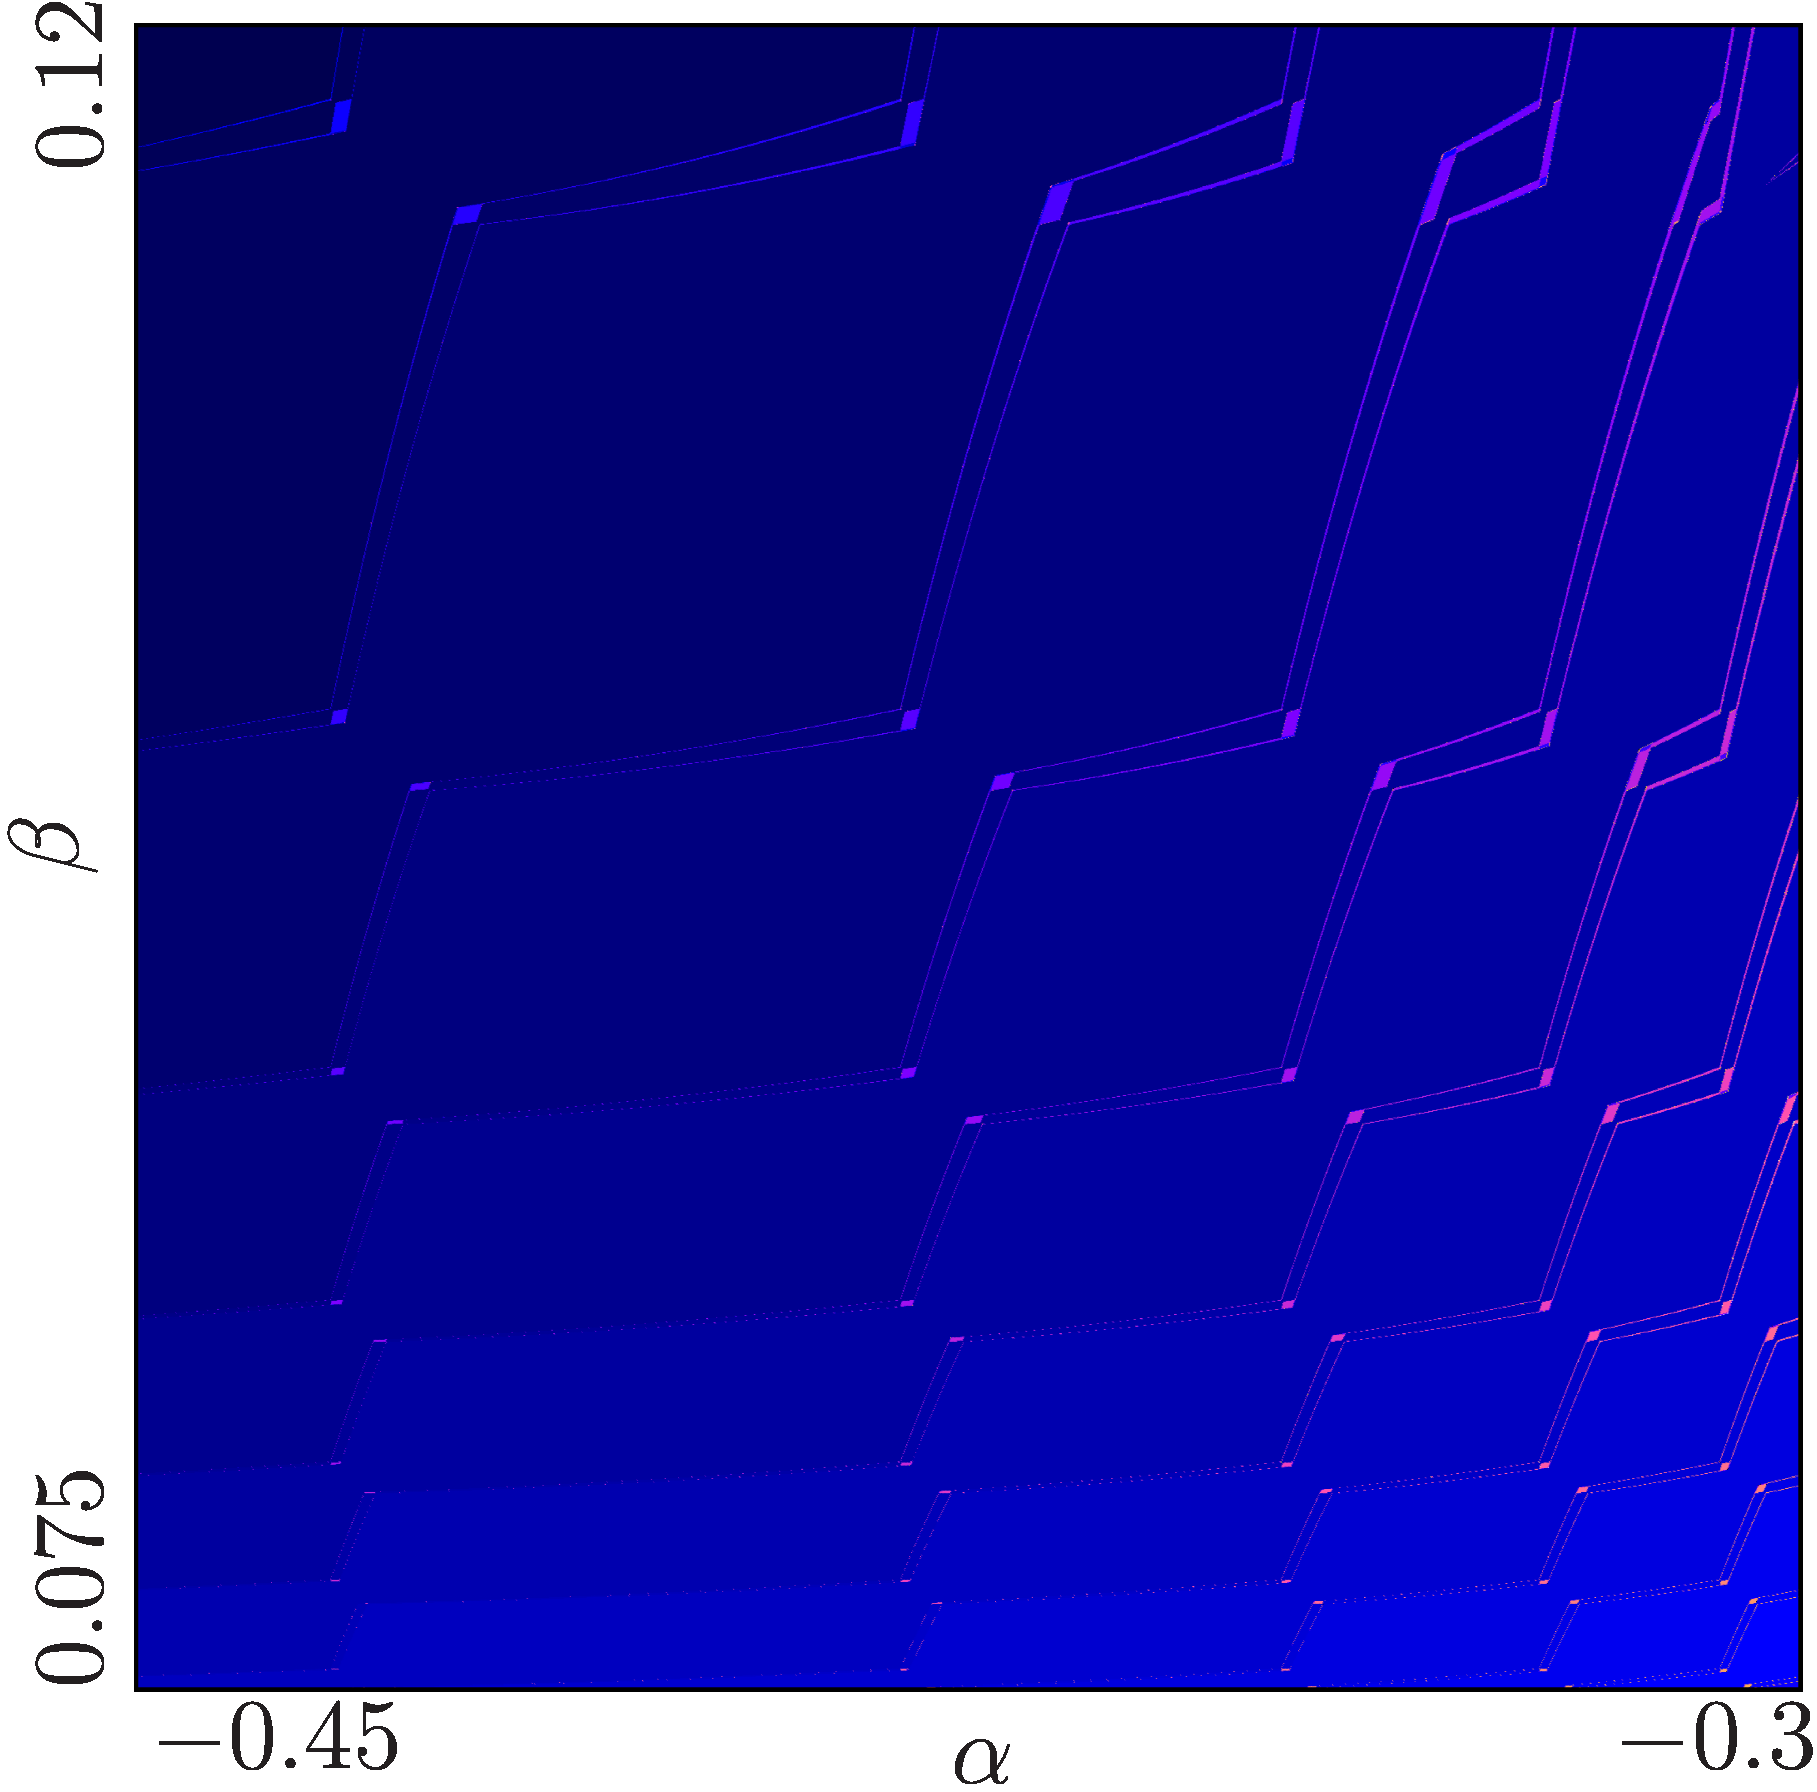
\includegraphics[width=.6 \textwidth]{../Figures/7/7.1/result.png}
	\caption[2D period scan of the piecewise-increasing increasing archetypal model]{
		2D period scan of the piecewise-increasing increasing archetypal model.
		With the fixed parameters $a_L = 1, b_L = \frac{1}{2},$ and $g_R\left(\frac{1}{2}\right) = \frac{1}{2} + \frac{1}{40}$.
		The parameters $\alpha = g_R\left(\frac{1}{4}\right)$ and $\beta = c_L$ are varied.
	}
	\label{fig:add.arch.new.period}
\end{figure}

\begin{figure}
	\centering
	\subfloat[Skew sawtooth map]{
		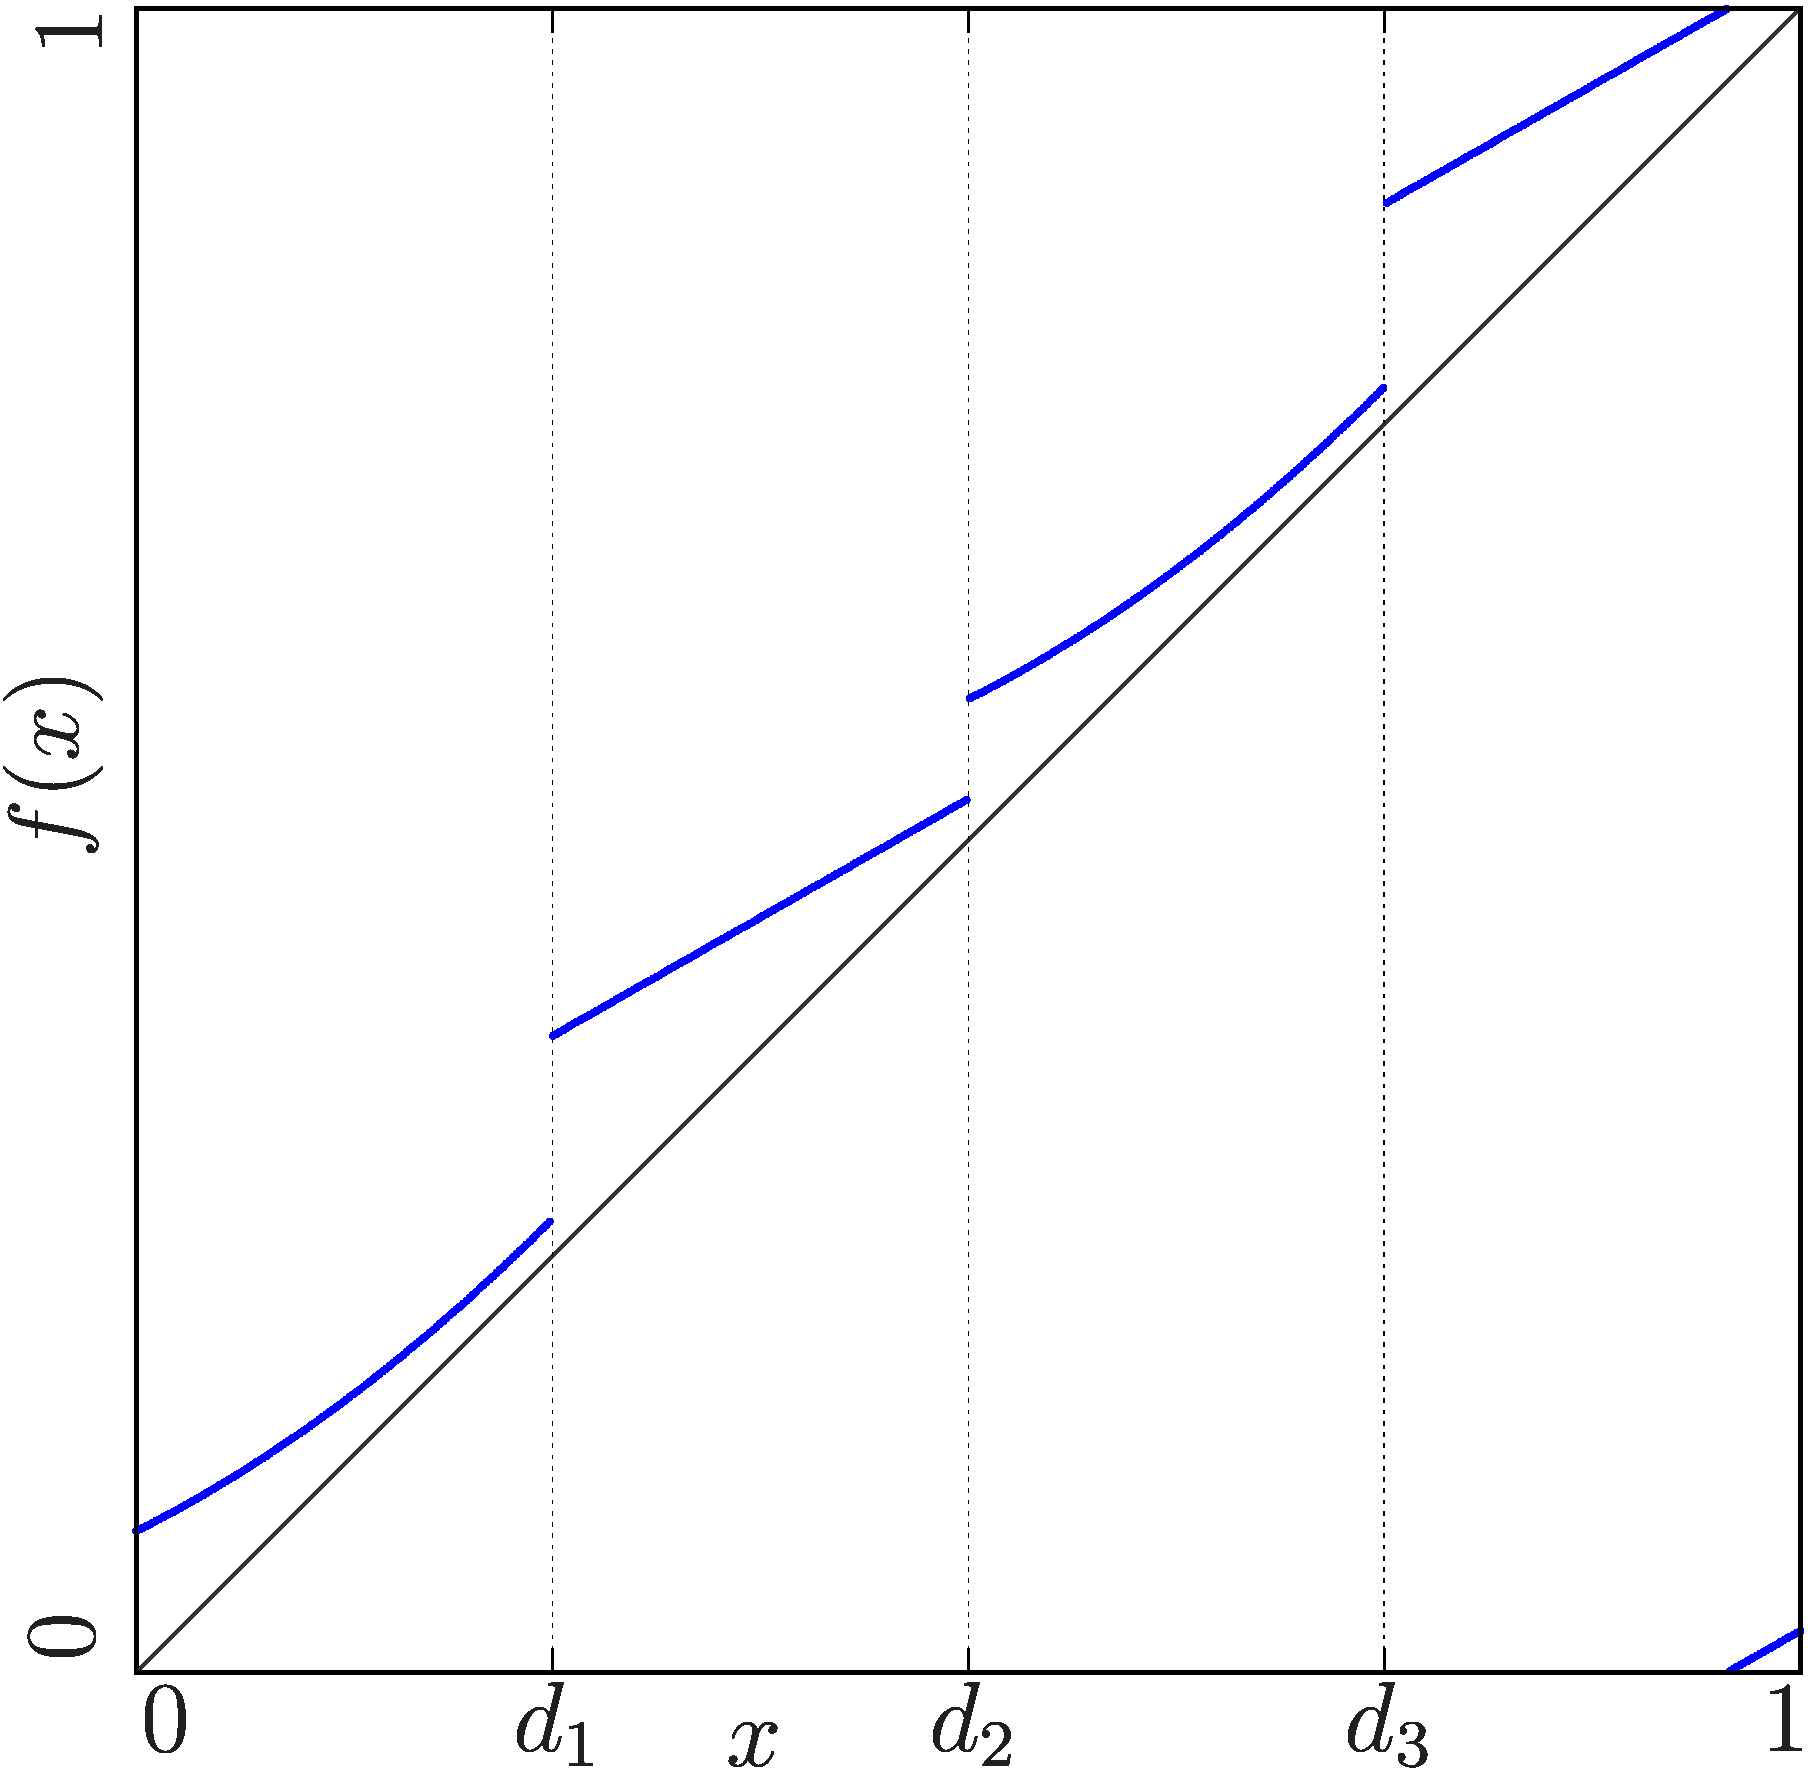
\includegraphics[width=.4 \textwidth]{../Figures/7/7.2a/result.png}
		\label{fig:add.saw}
	}
	\subfloat[Function shape]{
		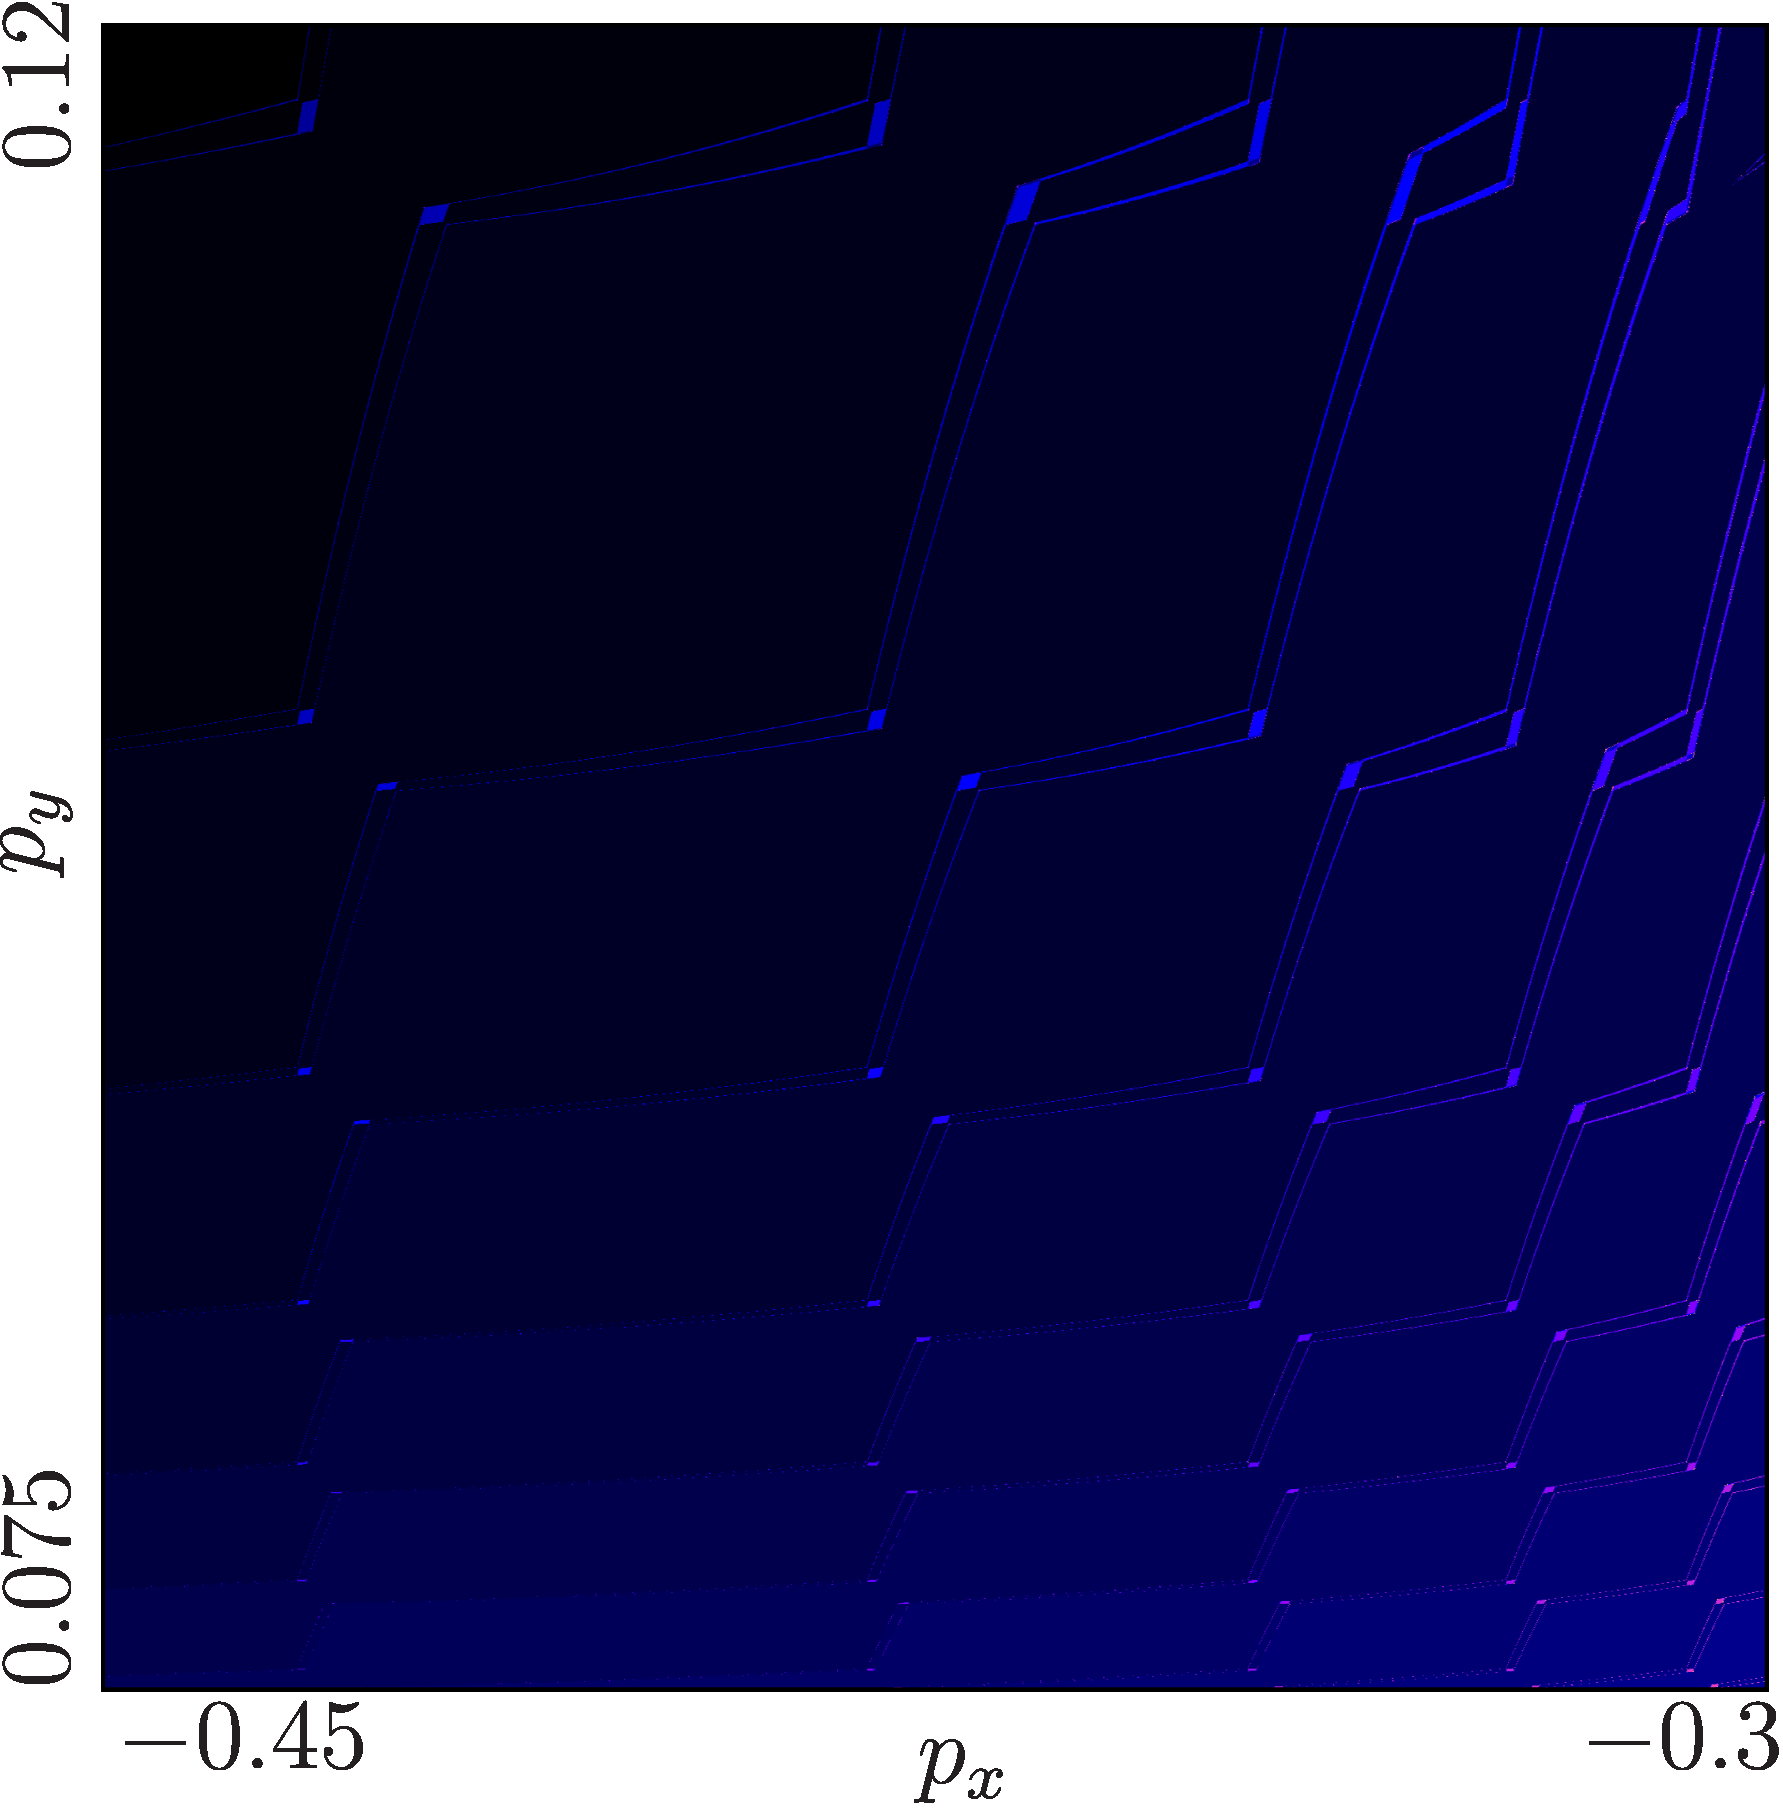
\includegraphics[width=.4 \textwidth]{../Figures/7/7.2b/result.png}
		\label{fig:add.arch.new}
	}
	\caption[Comparison of the piecewise-increasing archetypal model function and the skew sawtooth map]{
		Comparison of the piecewise-increasing archetypal model function and the skew sawtooth map.
		(a) shows the archetypal model function with the parameters $a_L = 1, b_L = \frac{1}{2}, c_L = 0.168, g_R\left(\frac{1}{4}\right) = -0.4 ,$ and $g_R\left(\frac{1}{2}\right) = \frac{1}{2} + \frac{1}{40}$.
		(b) shows the skew sawtooth map \hl{which is defined in} \cite{simpson2018saw} with the parameters $a_L = 0.5$ and $a_R = 1.5$.
		The parameters happen to have similar names to the parameters of the archetypal model.
	}
	\label{fig:add.saw.vs.arch}
\end{figure}

\section{Changes to the Bifurcation Structure}
\label{sec:add.change}

This section examines how changing the parameters as described in \Cref{sec:add.parameters} changes the bifurcation structure of the archetypal model.

\subsection{Numerical Overview of the Changes to the Bifurcation Structure}
\label{sec:add.change.num}

\Cref{fig:add.change.regions} shows diagrams depicting the borders of parameter regions with different symbolic sequences.
These diagrams are used as the basis for the exploration of changes to the bifurcation structure.
The lower left corner of the diagrams is always in the period region with the stable cycle $\Cycle{\A^7\B^3\C^7\D^3}$.
The cycles in the upper left ($\Cycle{\A^6\B^3\C^6\D^3}$), upper right ($\Cycle{\A^6\B^4\C^6\D^4}$), lower right ($\Cycle{\A^7\B^4\C^7\D^4}$), and middle ($\Cycle{\A^7\B^3\C^6\D^4}$ and $\Cycle{\A^6\B^4\C^7\D^3}$) follow.

Here, a short notation for the symbolic sequences is introduced.
``Type A'' parameter regions where the cycle is associated with the symbolic sequence $\A^a\B^b\C^a\D^b$ are written as $P^{2 \cdot \left(a + b\right)}_b$
``Type B'' parameter regions where the coexisting twin cycles are associated with the symbolic sequences $\A^a\B^b\C^c\D^d$ and $\A^c\B^d\C^a\D^b$ where $c = a - 1$ and $d = b + 1$ are written as $P^{a + b + c + d}_b$.
So for example, the ``type A'' parameter region in the lower left corner of every diagram in \Cref{fig:add.change.regions} is written as $P^{20}_3$.

There is also a new type of parameter region that we call hybrid parameter regions with hybrid cycles.
Hybrid cycles are cycles that are asymmetrical like ``type B'' cycles and therefore also exist in pairs.
The difference to ``type B'' cycles is that for two hybrid twin cycles with the symbolic sequences $\A^a\B^b\C^c\D^d$ and $\A^c\B^d\C^a\D^b$ either $c \neq a - 1$ or $d \neq b + 1$ but $c \leq a$ and $d \geq b$.
For example, the two hybrid twin cycles $\Cycle{\A^7\B^4\C^6\D^4}$ and $\Cycle{\A^6\B^4\C^7\D^4}$.
Their corresponding parameter region is written  in the short notation.
The short notation for their corresponding parameter regions is $P^{22}_4$ and $P^{20}_4$, respectively.
The parameter region with such hybrid cycles is written as $\left[P^{22}_4 \mid P^{20}_4\right]$.
This notation is chosen because of an operation that is introduced in the later \Cref{sec:add.add.halved}.
\Cref{sec:add.change.appa} covers how these parameter regions are created.
These parameter regions are connected to the \gls{pal} structures next to them, as we will see later in \Cref{sec:add.add.halved}.

The four different diagrams in \Cref{fig:add.change.regions} show the evolution at different points during the transition from the archetypal model to the piecewise-increasing archetypal model.
For this, the parameter values for $a_L$ and $b_L$ are chosen along a line given by \Cref{equ:add.change.paramline}.
\begin{align}
	a_L = \frac{5}{2} - 3 \cdot b_L
	\label{equ:add.change.paramline}
\end{align}

\begin{figure}
	\centering
	\subfloat[$a_L = 3.5, b_L = -0.\overline{3}$]{
		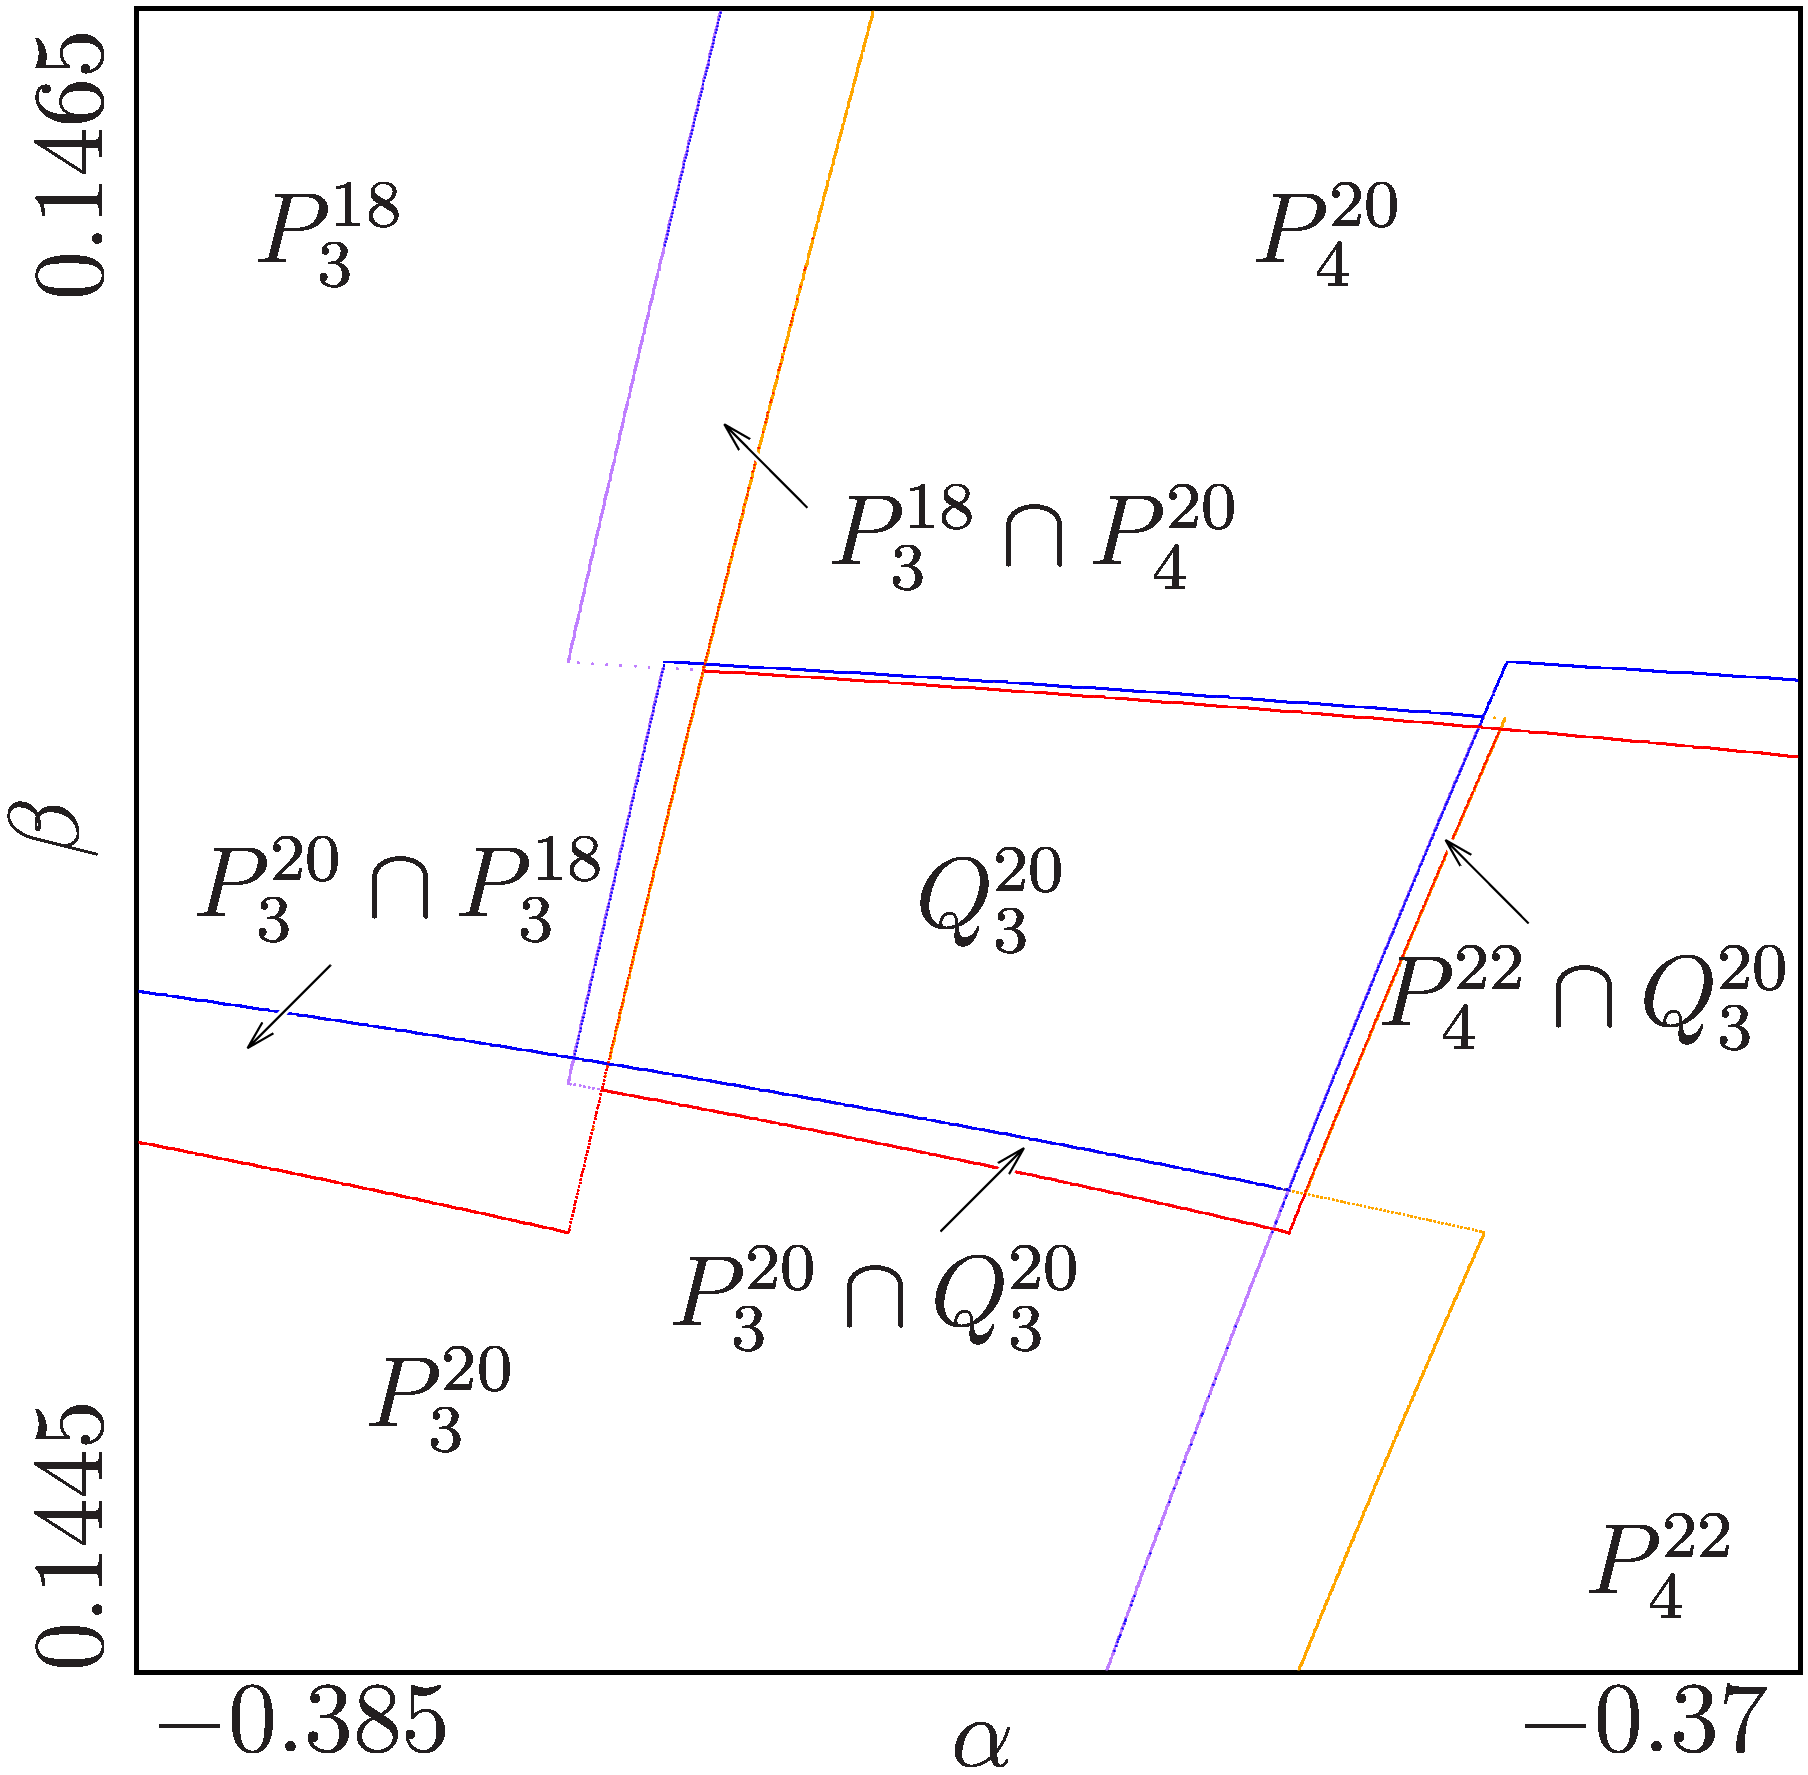
\includegraphics[width=.45 \textwidth]{../Figures/7/7.3a/result.png}
		\label{fig:add.change.regions.1}
	}
	\subfloat[$a_L = 2.8, b_L = -0.1$]{
		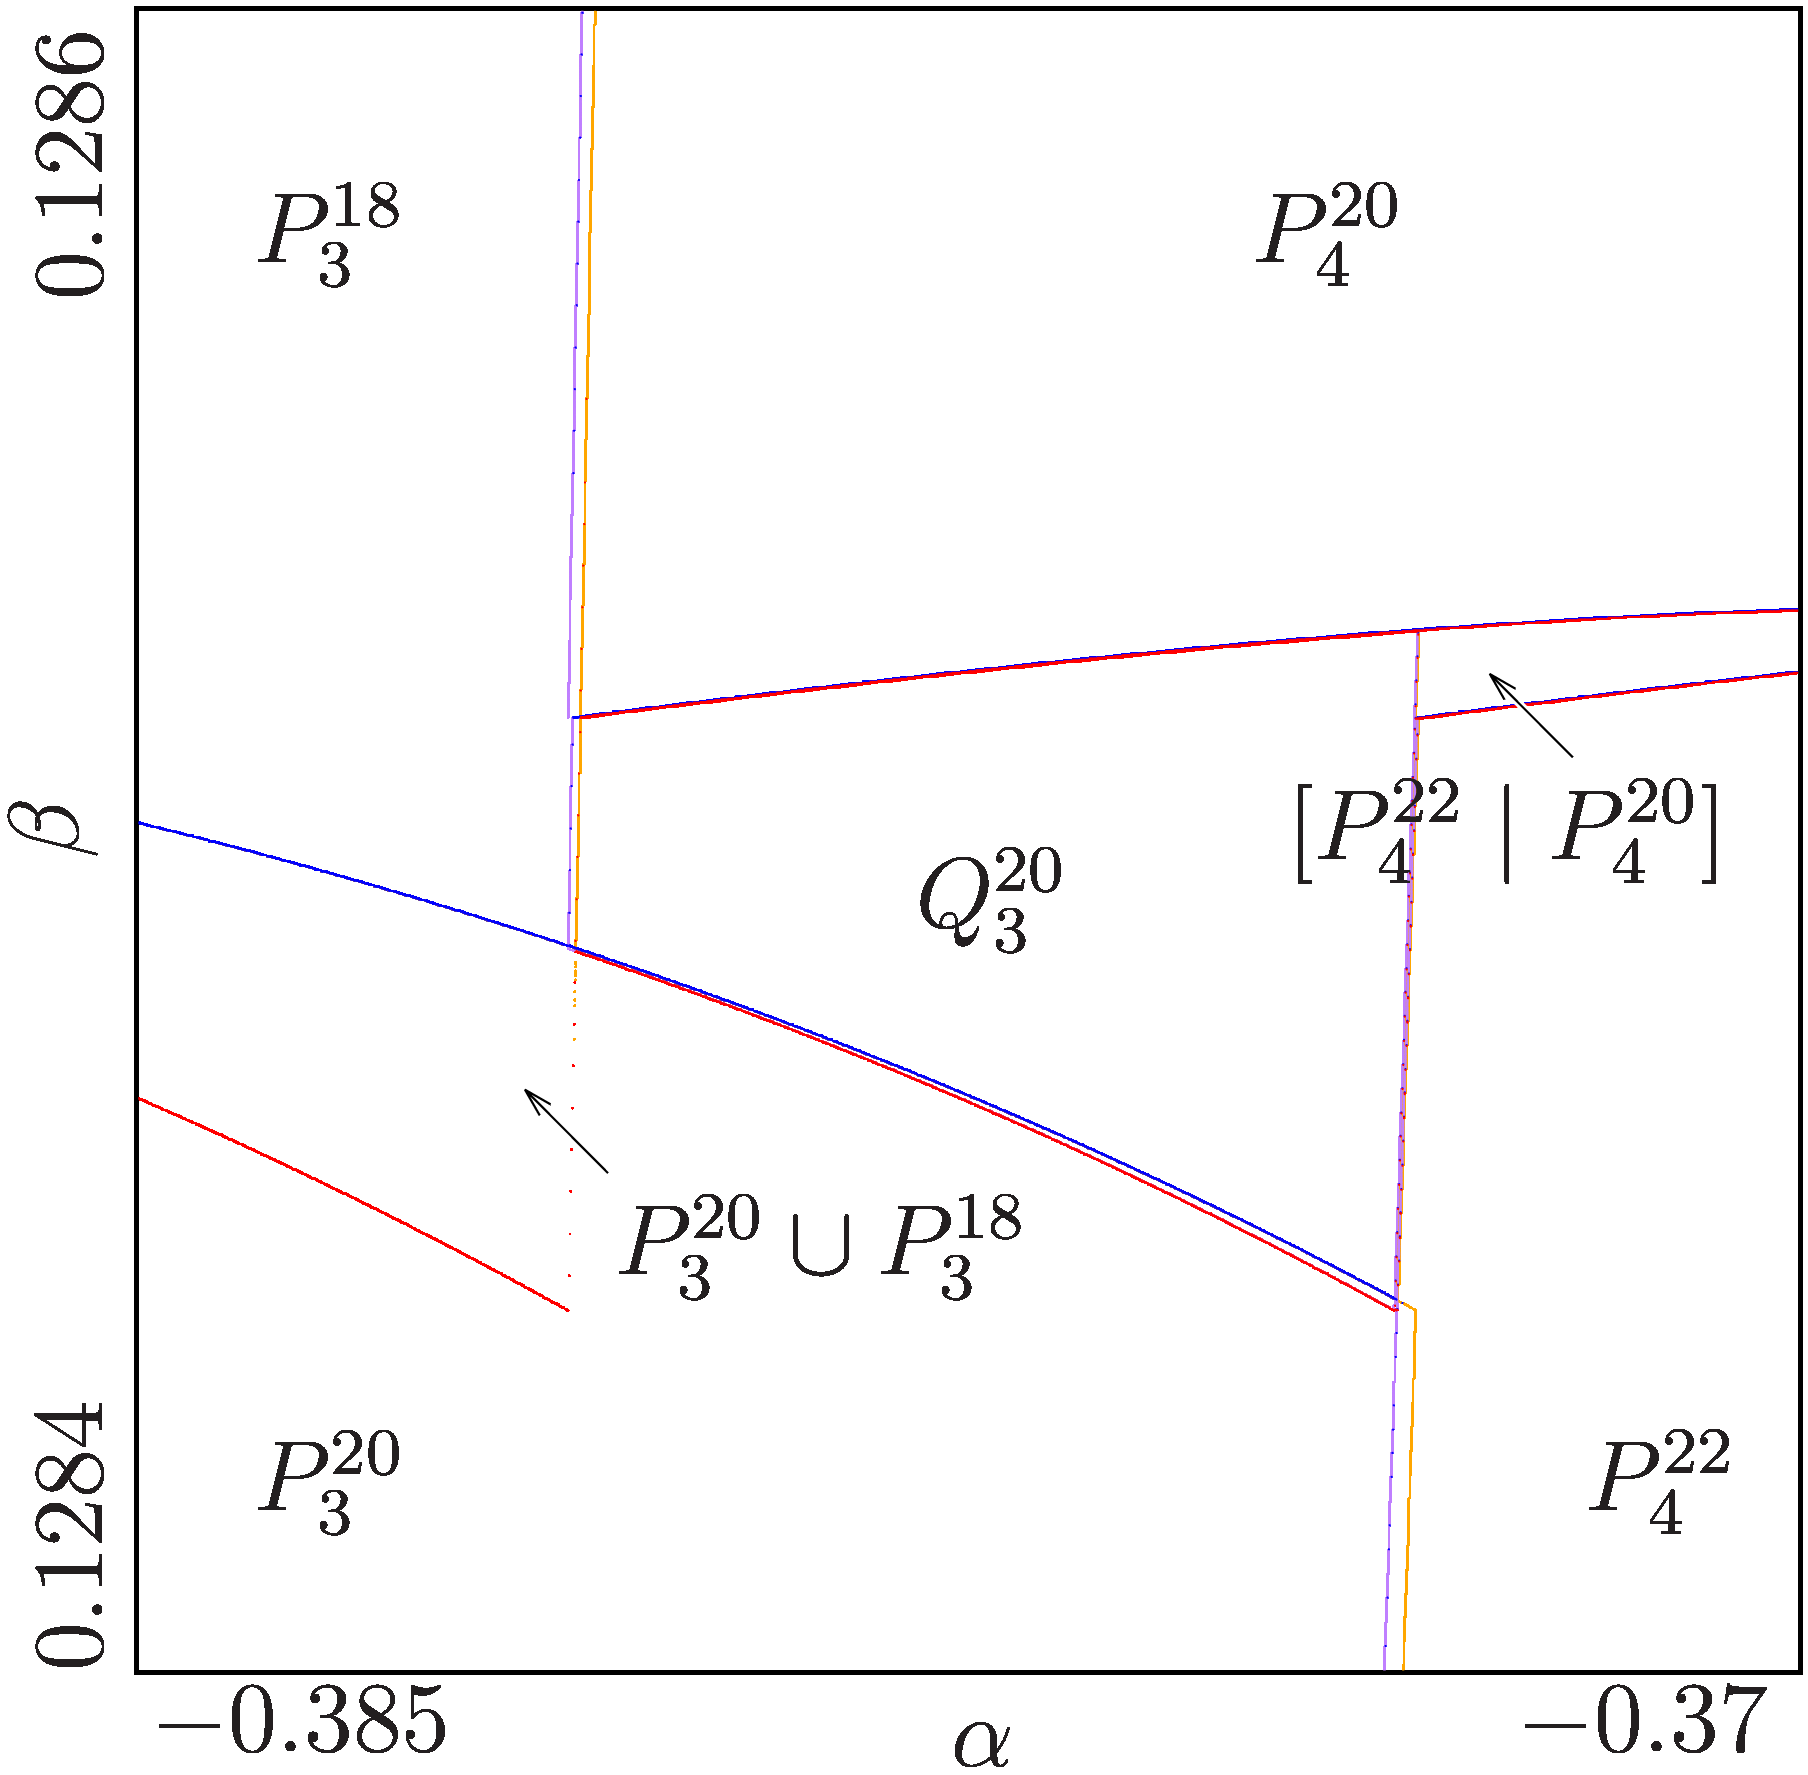
\includegraphics[width=.45 \textwidth]{../Figures/7/7.3b/result.png}
		\label{fig:add.change.regions.2}
	} \\
	\subfloat[$a_L = 2.725, b_L = -0.075$]{
		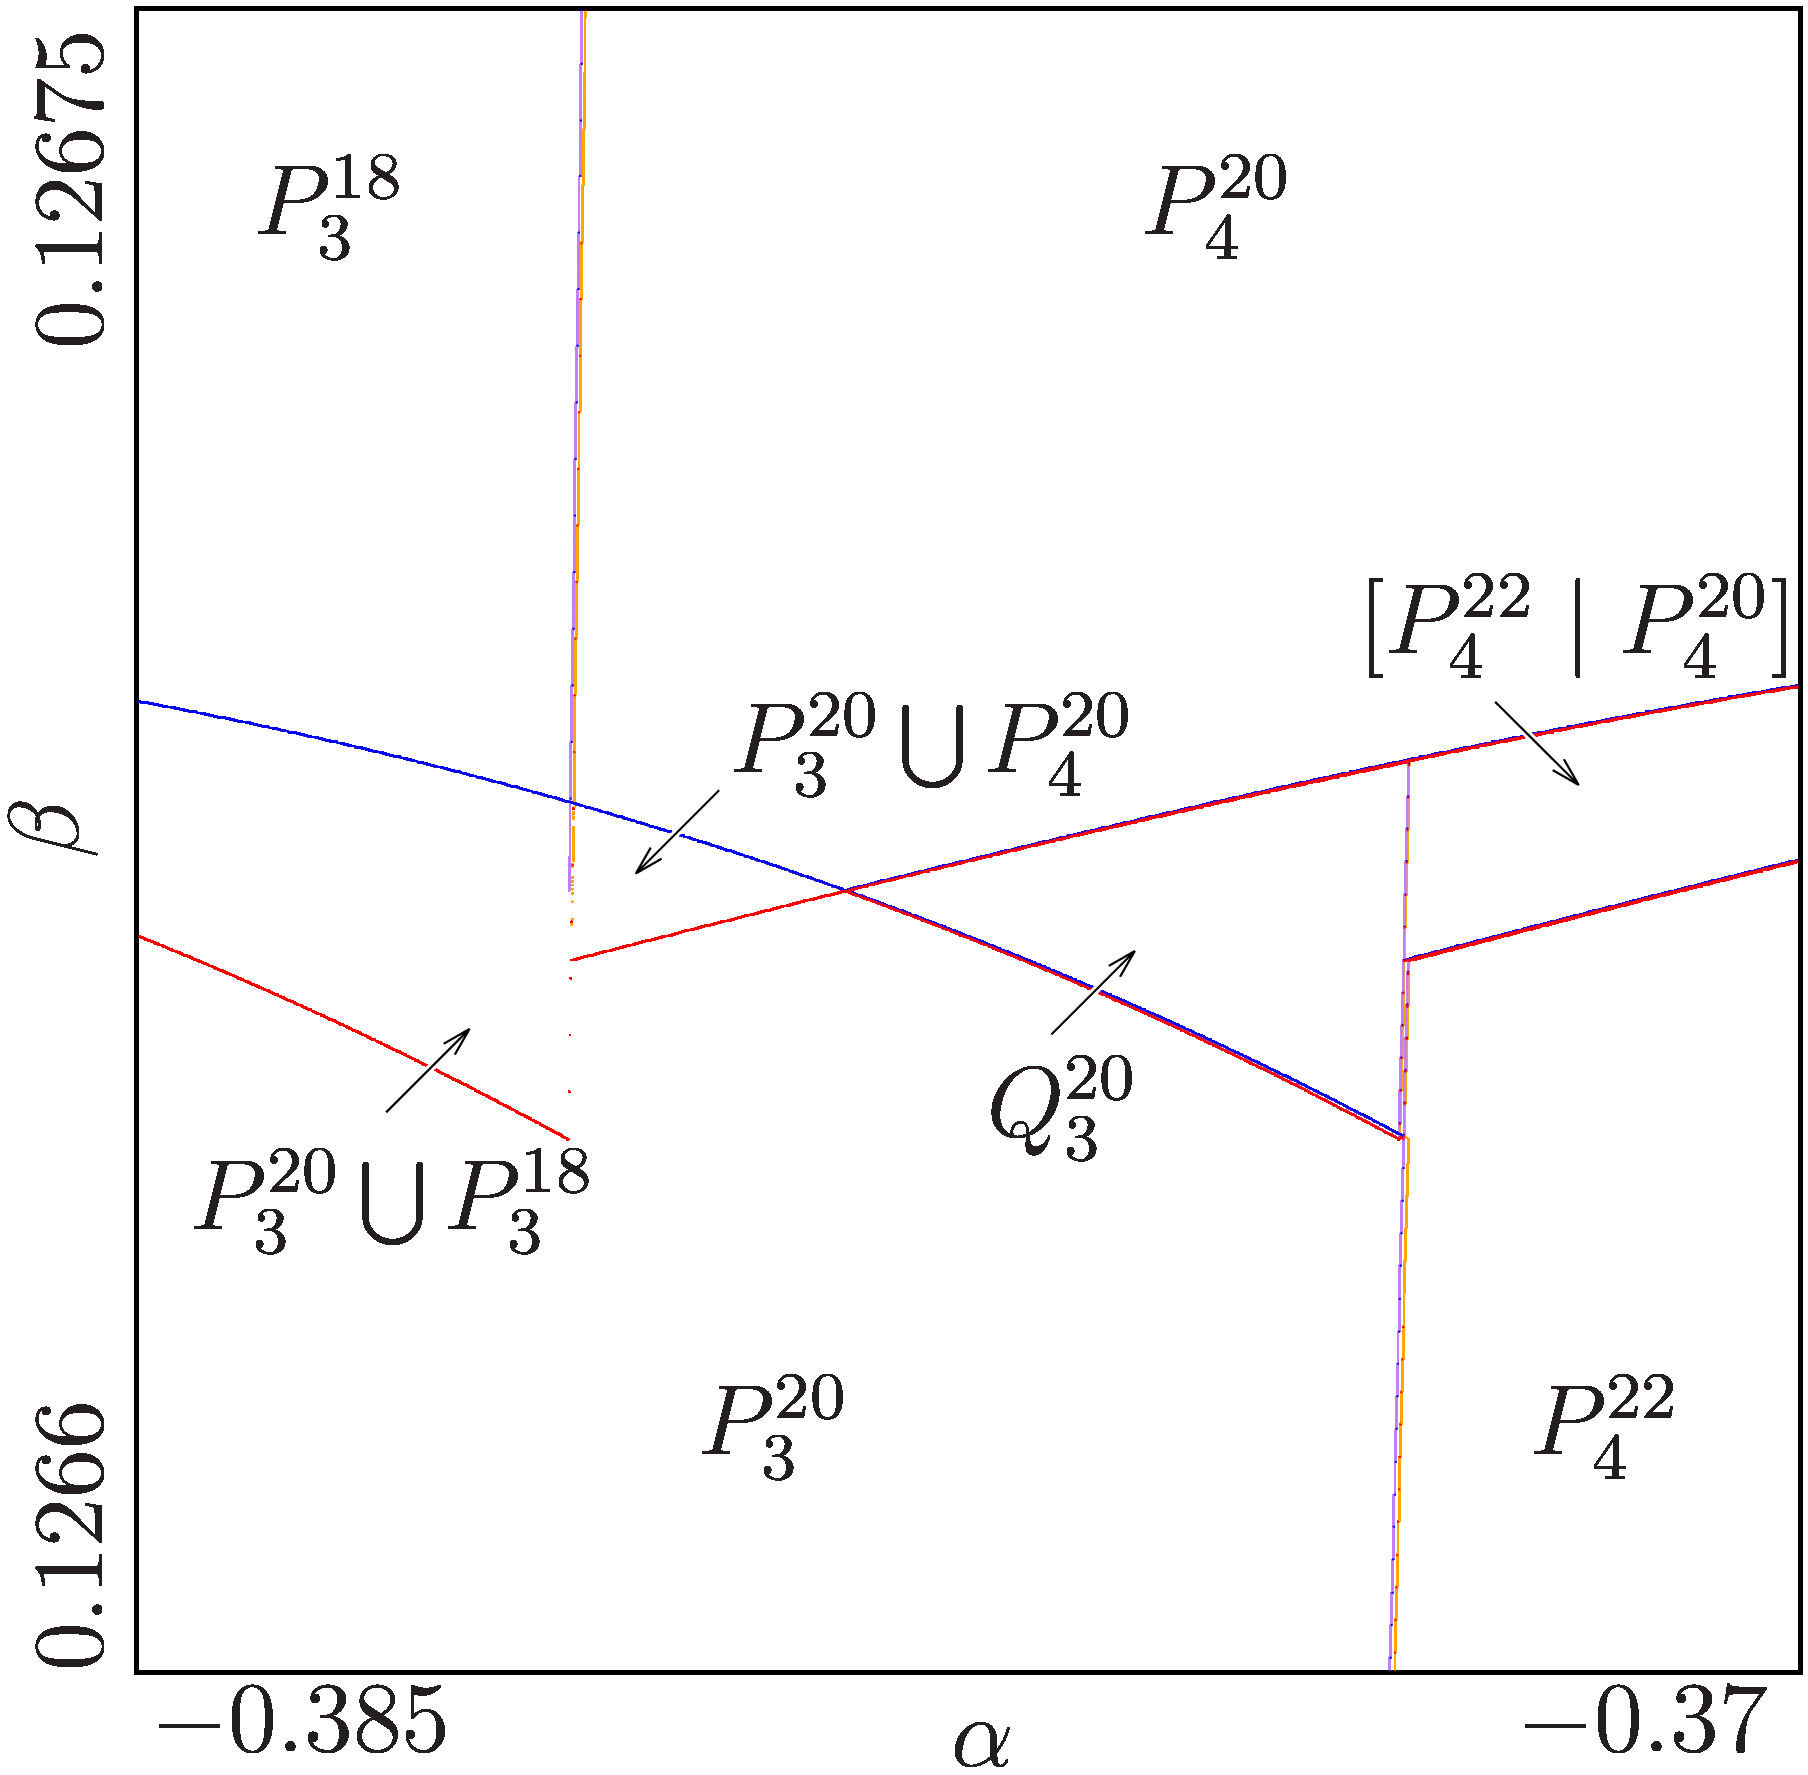
\includegraphics[width=.45 \textwidth]{../Figures/7/7.3c/result.png}
		\label{fig:add.change.regions.3}
	}
	\subfloat[$a_L = 2.5, b_L = 0$]{
		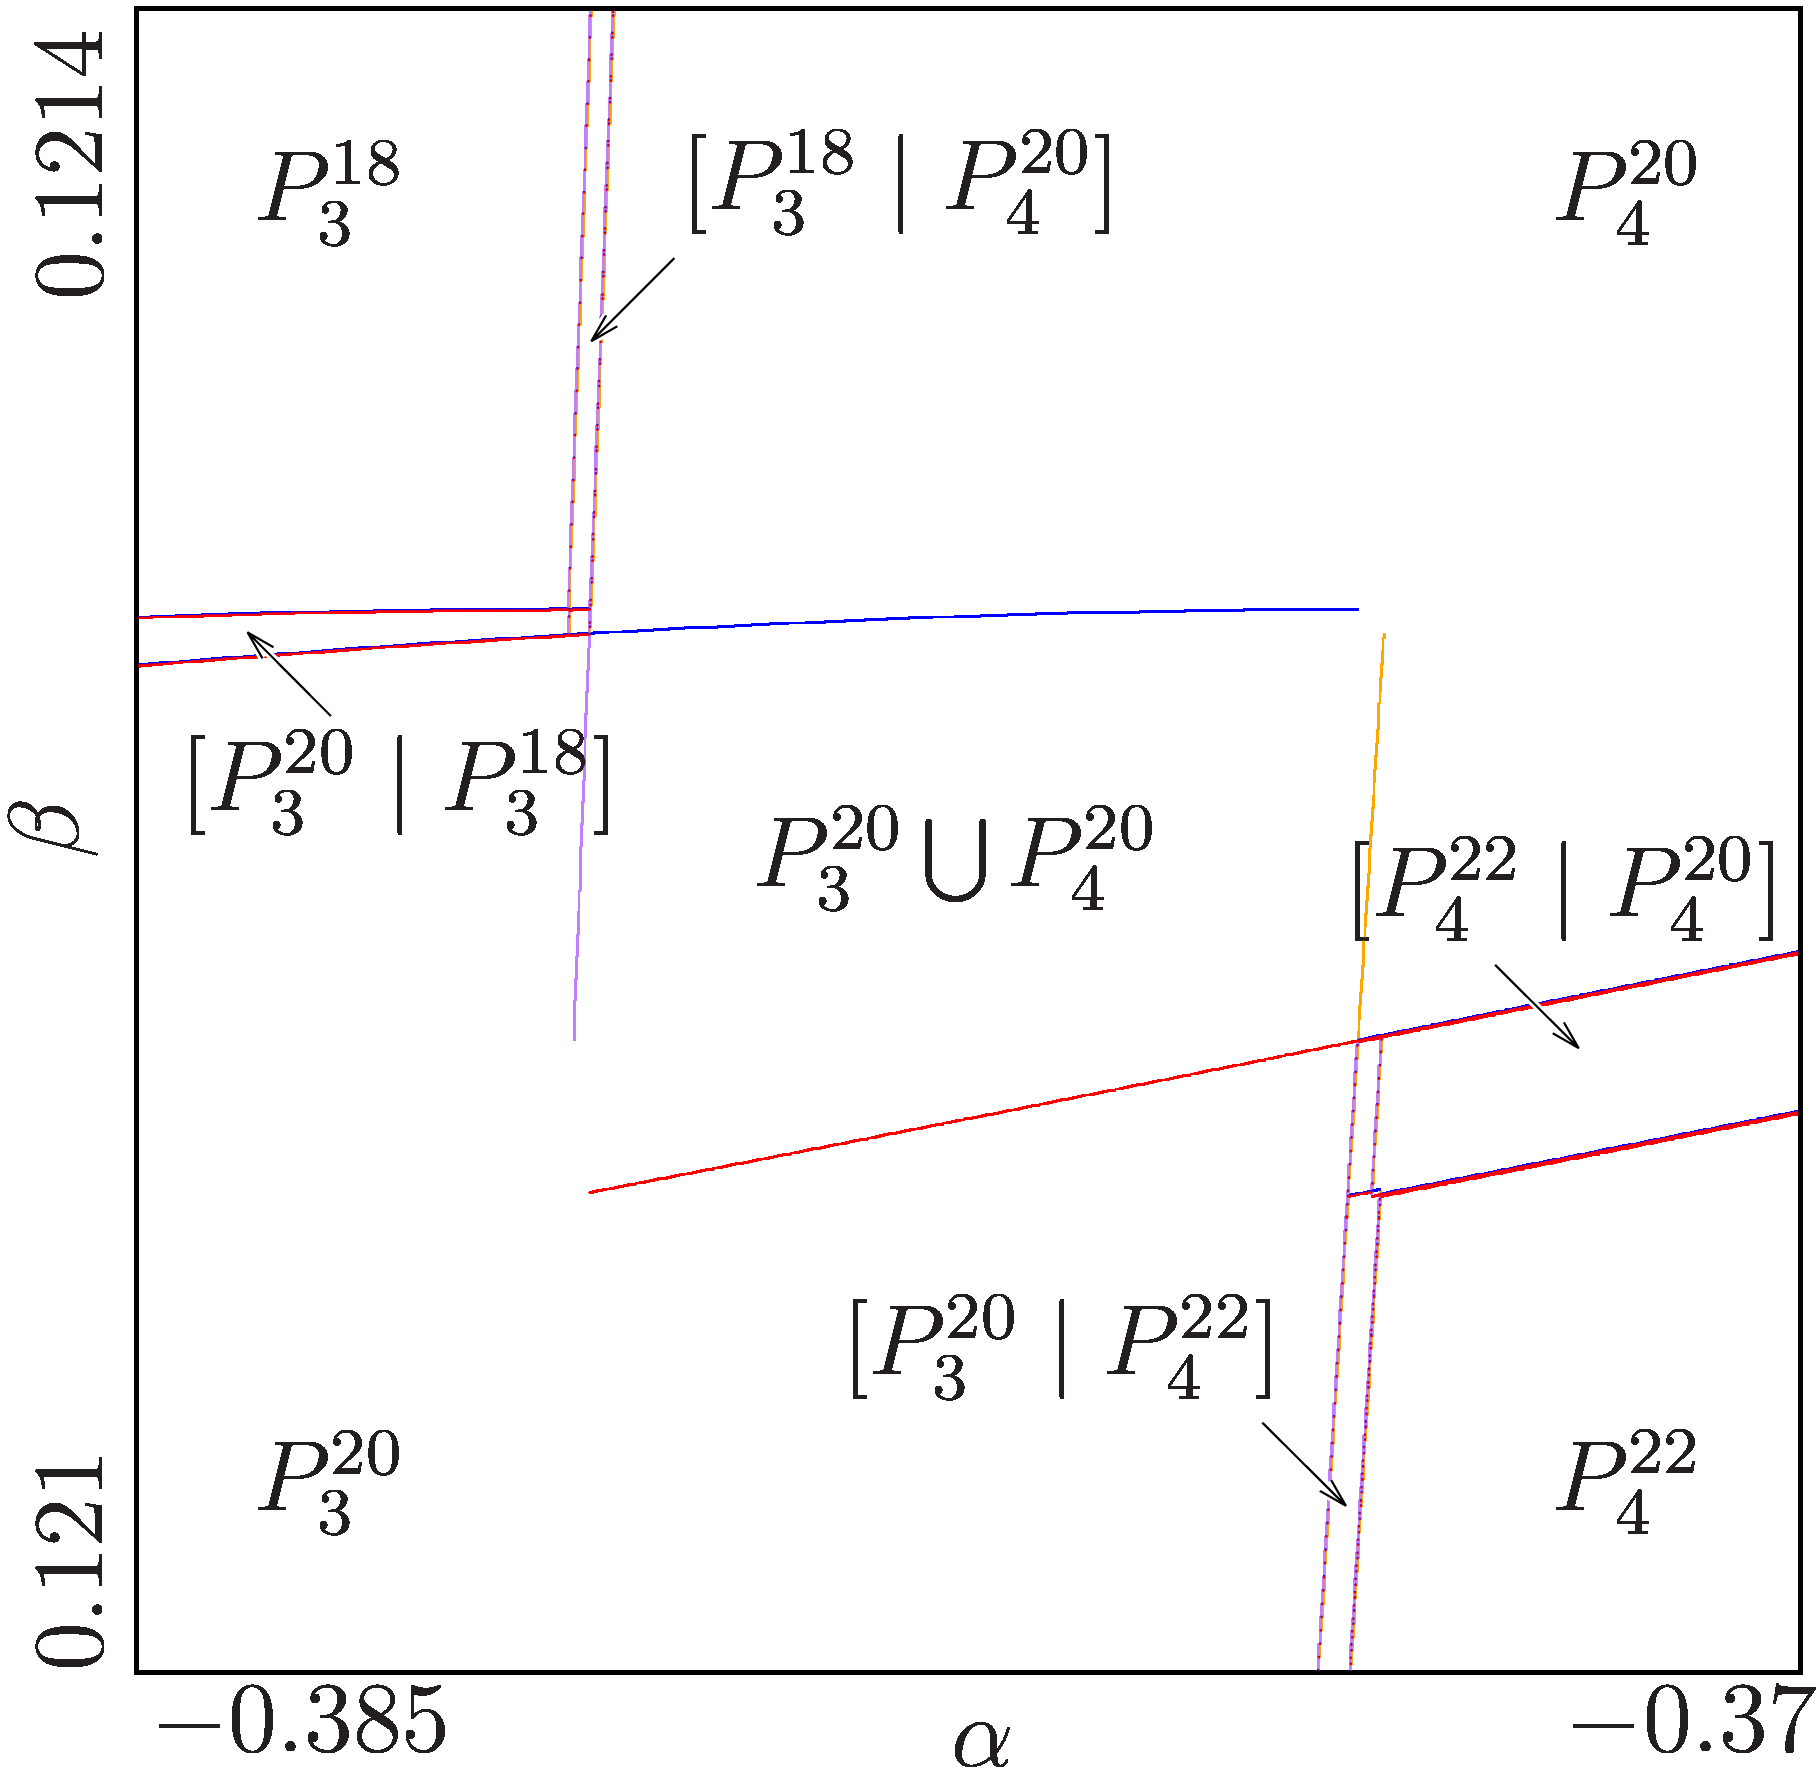
\includegraphics[width=.45 \textwidth]{../Figures/7/7.3d/result.png}
		\label{fig:add.change.regions.4}
	}
	\caption[2D scans of the boundaries of parameter regions associated with different symbolic sequences in the archetypal model showing their evolution when transitioning to increasing branches]{
		2D scans of the boundaries of parameter regions associated with different symbolic sequences in the archetypal model showing their evolution when transitioning to increasing branches.
		The parameter $g_R\left(\frac{1}{2}\right) = \frac{1}{2} + \frac{1}{40}$ is fixed in every diagram.
		The parameters $a_L$ and $b_L$ are fixed, but different in every diagram.
		Their values are on the line given by \Cref{equ:add.change.paramline}.
		The parameter $\alpha = g_R\left(\frac{1}{4}\right)$ is varied in the range $[-0.385, -0.37]$ in every diagram.
		The parameter $\beta = c_L$ is varied in different ranges in every diagram such that the parameter region in the lower left corner is always $P^{20}_3$.
		(a) shows the boundaries for the fixed parameters $a_L = 3.5$ and $b_L = -0.\overline{3}$ with the parameter $\beta$ being varied in the range $[0.1445, 0.1465]$,
		(b) shows the boundaries for the fixed parameters $a_L = 2.8$ and $b_L = -0.1$ with the parameter $\beta$ being varied in the range $[0.1284, 0.1286]$,
		(c) shows the boundaries for the fixed parameters $a_L = 2.75$ and $b_L = -0.075$ with the parameter $\beta$ being varied in the range $[0.1266, 0.12675]$,
		and (d) shows the boundaries for the fixed parameters $a_L = 2.5$ and $b_L = 0$ with the parameter $\beta$ being varied in the range $[0.121, 0.1214]$.
	}
	\label{fig:add.change.regions}
\end{figure}

The disappearance of the ``type B'' parameter regions is examined first in the next section.
The section after that examines the appearance of the \gls{pal} structures between the chains of parameter regions associated with the same period.

\clearpage
\subsection{Disappearance of ``Type B'' Parameter Regions}
\label{sec.change.disb}

For \Cref{fig:add.change.regions.1,fig:add.change.regions.2}, the ``type B'' parameter region $Q^{20}_3$ is complete.
In \Cref{fig:add.change.regions.4}, it is gone completely, instead the two ``type A'' parameter regions $P^{20}_3$ and $P^{20}_4$ now overlap.
\todo{In regions figure 3: labels $P^{20}_2$ wrong, should be $P^{20}_4$}

In between those two stages, we can see how the ``type B'' parameter region $Q^{20}_3$ disappears.
\Cref{fig:add.change.regions.3} shows the ``type A'' parameter regions $P^{20}_3$ and $P^{20}_4$ overlapping.
The point, where their boundaries cross is in the middle of where the ``type B'' parameter region was in \Cref{fig:add.change.regions.2}.
This point is also where the ``type B'' parameter region now ends.

\todo{Labels in figure wrong!}
\todo{In cobweb diagrams: enhance cycles at borders}
\begin{figure}
	\centering
	\subfloat[Regions]{
		\includegraphics[width=.3 \textwidth]{62_MinimalRepr_Adding/2D_Regions_2.675/Manual/result.png}
		\label{fig:add.change.disb.regions}
	}
	\subfloat[Cobweb at point $A$]{
		\includegraphics[width=.3 \textwidth]{62_MinimalRepr_Adding/Cob_2.675_A/Manual/result.png}
		\label{fig:add.change.disb.cob.A}
	}
	\subfloat[Cobweb at point $B$]{
		\includegraphics[width=.3 \textwidth]{62_MinimalRepr_Adding/Cob_2.675_B/Manual/result.png}
		\label{fig:add.change.disb.cob.B}
	}
	\caption{Disappearance of the ``type B'' parameter region}
\end{figure}

\Cref{fig:add.change.disb.regions} shows the same thing as \Cref{fig:add.change.regions.3} again but at parameter value closer to the diappearence of the ``type B'' parameter region.
We can see that the point where the boundaries of the ``type A'' parameter regions cross moved right and the ``type B'' parameter region got smaller.
This point is called a codimension-2 point because at this point, two bifurcations happen at the same time to the same cycle.

We know from \Cref{sec:arch.bif.sum} that the \gls{bcb} at the upper boundary of the ``type A'' parameter region $P^{20}_3$ is $\BCB_{d_1, d_3}^{\underline{\A}^7\B^3\underline{\C}^7\D^3}$.
And the \gls{bcb} at the lower boundary of the ``type A'' parameter region $P^{20}_4$ is $\BCB_{d_1, d_3}^{\A^6\underline{\B}^4\C^6\underline{\D}^4}$.
At the codimension-2 point, both these \glspl{bcb} happen at the same time and both cycles vanish.
We can see in \Cref{fig:add.change.disb.cob.A} that the ``type A'' cycles are very close to the borders $d_1$ and $d_3$, respectively.

We also know that the \glspl{bcb} at the top of the ``type B'' parameter region $Q^{20}_3$ are $\BCB_{d_1}^{\underline{\A}^7\B^3\C^6\D^4}$ and $\BCB_{d_3}^{\A^6\B^4\underline{\C}^7\D^3}$.
And the \glspl{bcb} at the lower boundary are $\BCB_{d_3}^{\A^7\B^3\C^6\underline{\D}^4}$ and $\BCB_{d_1}^{\A^7\underline{\B}^3\C^6\D^4}$.
At the codimension-2 point, both \glspl{bcb} $\BCB_{d_1}^{\underline{\A}^7\B^3\C^6\D^4}$ and $\BCB_{d_3}^{\A^7\B^3\C^6\underline{\D}^4}$ happen to the cycle $\Cycle{\A^7\B^3\C^6\D^4}$ at the same time and it vanishes.
Because of the symmetry, the \glspl{bcb} $\BCB_{d_3}^{\A^6\B^4\underline{\C}^7\D^3}$ and $\BCB_{d_1}^{\A^7\underline{\B}^3\C^6\D^4}$ happen to the cycle $\Cycle{\A^6\B^4\C^7\D^3}$ at the same time and it vanishes also.

This codimension-2 point moves right with higher values for $b_L$ along our line.
As soon as the codimension-2 point crosses the right boundary of the ``type B'' parameter region, the ``type B'' parameter region ceases to exist.
Instead, now the two ``type A'' parameter regions overlap without the codimension-2 point.
This new overlapping regions is bounded by simple ``type A'' boundary \glspl{bcb} as they are discussed in \Cref{sec:arch.bif.sum}.

\todo{Confirm bcbs with cobweb diagrams}

\todo{Order of left most cycle and other cycle => type B or type A. idk}

\subsection{Appearance of Period-adding structures}

In this section we will explore the appearance of the period-adding structures in between the chains of the same period.
This happens at the horizontal boundaries between ``type A'' parameter regions of different chains, as well as at the vertical boundaries.
We will first take care of the horizontal period-adding structures and then move on to the vertical period-adding structures.

\subsubsection{Horizontal Period-adding Structures}

In \Cref{fig:add.change.regions.1}, the ``type A'' parameter regions $P^{20}_3$ and $P^{18}_3$, as well as $P_{22}_4$ and $P^{20}_4$ overlap.
This changes in \Cref{fig:add.change.regions.2}.
Here only the ``type A'' parameter regions $P^{20}_3$ and $P^{18}_3$ overlap, the parameter regions $P_{22}_4$ and $P^{20}_4$ stopped overlapping.
Instead, in the space between the two ``type A'' parameter region there are now two asymmetric coexisting twin cycles $\Cycle{\A^8\B^3\C^8\D^2}$ and $\Cycle{\A^8\B^2\C^8\D^3}$.
Those cycles are \textbf{not} ``type B'' cycles, because they only differ in the number of points on the branches $f_\B$ and $f_\D$.
Instead, we will call them hybrid cycles and ``type B'' cycles are a special case of hybrid cycles.
The notation $\left[P^{22}_4 \mid P^{20}_4\right]$ used in the diagrams was introduced in \Cref{sec:add.change} and is formally defined later in \Cref{sec:add.add.halved}.
Later in \Cref{fig:add.change.regions.4}, the ``type A'' parameter regions $P^{20}_3$ and $P^{18}_3$ also stop overlapping.
In between, there are also hybrid cycles, $\Cycle{\A^7\B^3\C^6\D^3}$ and $\Cycle{\A^6\B^3\C^7\D^3}$.
This parameter region is therefore labeled $\left[P^{20}_3 \mid P^{18}_3\right]$.

In between \Cref{fig:add.change.regions.2,fig:add.change.regions.3}, the ``type A'' parameter regions $P_{22}_4$ and $P^{20}_4$ don't stop overlapping completely.
Instead, they only stop overlapping on the left side of their shared boundaries and the rest is not pictured in these diagrams.
\Cref{fig:add.change.appa.hor.regions} shows better what happens to this overlapping region between \Cref{fig:add.change.regions.1,fig:add.change.regions.4}.
We also have a codimension-2 point that moves right as was the case in \Cref{sec:add.change.disb}.

\todo{Regions: labels wrong}
\todo{Cobwebs: enhance borders, replace (c), wrong pic}
\begin{figure}
	\centering
	\subfloat[Regions]{
		\includegraphics[width=.3 \textwidth]{62_MinimalRepr_Adding/2D_Regions_2.8_add_hor/Manual/result.png}
		\label{fig:add.change.appa.hor.regions}
	}
	\subfloat[At point $A$]{
		\includegraphics[width=.3 \textwidth]{62_MinimalRepr_Adding/Cob_2.8_add_hor_A/Manual/result.png}
		\label{fig:add.change.appa.hor.cob.A}
	}
	\subfloat[At point $B$]{
		\includegraphics[width=.3 \textwidth]{62_MinimalRepr_Adding/Cob_2.8_add_hor_A/Manual/result.png}
		\label{fig:add.change.appa.hor.cob.B}
	}
	\caption{Appearance of the horizontal period-adding cascade}
\end{figure}

We know from \Cref{sec:arch.bif.sum} that the \gls{bcb} at the upper boundary of the ``type A'' parameter region $P^{22}_4$ is $\BCB_{d_1, d_3}^{\underline{\A}^7\B^4\underline{\C}^7\D^4}$.
And the \gls{bcb} at the lower boundary of the ``type A'' parameter region $P^{20}_4$ is $\BCB_{d_1, d_3}^{\A^6\underline{\B}^4\C^6\underline{\D}^4}$.
Both these \glspl{bcb} are at the upper and lower boundaries of the overlapping region $P^{22}_4 \Cup P^{20}_4$.
At the codimension-2 point, both these \glspl{bcb} happen at the same time and both cycles vanish.
We can see in \Cref{fig:add.change.appa.hor.cob.A} that the ``type A'' cycles are very close to the borders $d_1$ and $d_3$, respectively.

This codimension-2 point moves right with higher values for $b_L$ along our line.
As soon as the codimension-2 point crosses the right boundary of either the ``type A'' parameter region $P^{22}_4$ or $P^{20}_4$, the overlapping parameter region $P^{22}_4 \Cup P^{20}_4$ ceases to exist.
Instead, there is space between the two ``type A'' parameter regions where the are now two hybrid cycles and period-adding between the hybrid cycles and either ``type A'' parameter region.

\todo{Labels for bifurcations missing underline}
\begin{figure}
	\centering
	\includegraphics[width=.7 \textwidth]{62_MinimalRepr_Adding/1D_Bif_2.8_add_hor_AU/Manual/result.png}
	\caption{Bifurcation diagram at the upper boundary of $\left[P^{22}_4 \mid P^{20}_4\right]$}
	\label{fig:add.change.appa.hor.bif}
\end{figure}

We assume that the \glspl{bcb} bounding the parameter regions with hybrid cycles follow the same rules as the \glspl{bcb} bounding the ``type B'' parameter regions.
\Cref{fig:add.change.appa.hor.bif} confirms this for the upper boundary.
So it is bounded at the top by the \glspl{bcb} $\BCB_{d_1}^{\underline{\A}^7\B^4\C^6\D^4}$ and $\BCB_{d_3}^{\A^6\B^4\underline{\C}^7\D^4}$.
And bounded at the bottom by the \glspl{bcb} $\BCB_{d_3}^{\A^7\B^4\C^6\underline{\D}^4}$ and $\BCB_{d_1}^{\underline{\A}^6\B^4\C^7\D^4}$.
At the codimension-2 point, both \glspl{bcb} $\BCB_{d_1}^{\underline{\A}^7\B^4\C^6\D^4}$ and $\BCB_{d_3}^{\A^7\B^4\C^6\underline{\D}^4}$ happen to the cycle $\Cycle{\A^7\B^4\C^6\D^4}$ at the same time and it vanishes.
Because of the symmetry, the \glspl{bcb} $\BCB_{d_3}^{\A^6\B^4\underline{\C}^7\D^4}$ and $\BCB_{d_1}^{\A^6\underline{\B}^4\C^7\D^4}$ happen to the cycle $\Cycle{\A^6\B^4\C^7\D^4}$ at the same time and it vanishes also.

\todo{also confirmed by cobweb with enhanced cycles at borders}

\todo{Parallels to disappearing type B}

\todo{old:}

In \Cref{sec:minrep.adding.disapp.typeB}, we noted that the asymmetry of the ``type B'' cycles is caused by the negative slope of the function at the left border of branches $f_\A$ and $f_\C$.
Since this maps the cycle that starts further left to the right side of the other cycle.
\todo{
	explain better: diff number of points on branches B and D each (type B) therefore reordering necessary for asymm.
	type b also: split at $d_1, d_3$ as well as $d_2$ and $d_0$, here only $d_1, d_3$ (two boundaries).
	here same number of points so there must be no reordering for asymm
}
This is not the case for the cycles at this point, both cycles start at a point on the branch $f_\A$ with a positive slope and therefore keep the same order.
\todo{positive slope important for period adding!}

\subsubsection{Vertical}

\todo{Regions: labels wrong}
\todo{Cobwebs: replace (c) and enhance cycles at borders}
\begin{figure}
	\centering
	\subfloat[Regions scan before period-adding\\at $a_L = 2.8, b_L = -0.1$]{
		\includegraphics[width=.4 \textwidth]{62_MinimalRepr_Adding/2D_Regions_2.8_add_vert/Manual/result.png}
		\label{fig:minrep.add.app.vert.reg.before}
	}
	\subfloat[Regions with period-adding\\at $a_L = 2.65, b_L = -0.05$]{
		\includegraphics[width=.4 \textwidth]{62_MinimalRepr_Adding/2D_Regions_2.65_add_vert/Manual/result.png}
		\label{fig:minrep.add.app.vert.reg.with}
	} \\
	\subfloat[At point $A$]{
		\includegraphics[width=.4 \textwidth]{62_MinimalRepr_Adding/Cob_2.8_add_vert_A/Manual/result.png}
		\label{fig:minrep.add.app.vert.cob.A}
	}
	\subfloat[At point $B$]{
		\includegraphics[width=.4 \textwidth]{62_MinimalRepr_Adding/Cob_2.65_add_vert_B/Manual/result.png}
		\label{fig:minrep.add.app.vert.cob.B}
	}
	\caption{Appearance of the vertical period-adding cascade}
	\label{fig:minrep.add.app.vert}
\end{figure}

For the vertical period-adding cascade, it is similar.
This time one parameter region scan is not enough because the boundaries of $P_{10}^3$ and $P_{11}^4$ are parallel and therefor $P_{10}^3 \bigcup P_{11}^4$ and $P_{10}^3 \oplus P_{11}^4$ can't exist at the same parameter values of $a_L$ and $b_L$.
\Cref{fig:minrep.add.app.vert.reg.before} shows the situation before the vertical period-adding cascade appears.
Here we can see the overlap of the two ``type A'' parameter regions $P_{10}^3$ and $P_{11}^4$.
When changing the parameters a little, we get \Cref{fig:minrep.add.app.vert.reg.with}.
Here the two ``type A'' parameter regions drifted apart and in between them, there is the parameter region $P_{10}^3 \oplus P_{11}^4$.
The notation hints at the period-adding-like nature of this parameter region.

As with the horizontal period-adding cascade, the cycles here are asymmetrical, but not of ``type B''.
\Cref{fig:minrep.add.app.vert.cob.B} shows the cycles at point $B$, in the period adding cascade, $\Cycle{\A^7\B^3\C^7\D^4}$ and its twin $\Cycle{\A^7\B^4\C^7\D^3}$.
Again, interpreted in the context of the halved model, these cycles are both $\Cycle{\L^7\R^3\L^7\R^4} \equiv \Cycle{\L^7\R^4\L^7\R^3}$.
But this time, the splits are not at borders $d_1$ and $d_3$, but at $d_0$ and $d_2$.
\todo{odd number of splits => no neg slope needed for asymmetry. odd number => needed (reorders cycles)}

\begin{figure}
	\centering
	\includegraphics[width=.7 \textwidth]{62_MinimalRepr_Adding/1D_Bif_2.65_add_vert_BR/Manual/result.png}
	\caption{Bifurcation diagram of the right boundary of $P_{10}^3 \oplus P_{11}^4$}
	\label{fig:minrep.add.app.vert.bif.BR}
\end{figure}

Here, the period-adding region opened up enough to see the next stage, colored in purple.
As with the previous bifurcations of the first stage of the horizontal period-adding cascade, the bifurcations are similar to the bifurcations of ``type B'' cycles in \Cref{sec:minrep.bif.R}.
They involve the borders $d_0$ and $d_2$.
\todo{etc}

\subsection{Summary of the Changes to the Bifurcation Structure}

This section summarizes all the changes that happen to the \gls{pi} structure of the archetypal model when the parameters are changed in such a way that \gls{pal} structures emerge.
Furthermore, it provides an explanation for why the \gls{pi} structure of the archetypal model is impossible with only increasing branches.

\subsubsection{Schematics and Summary of the Changes}

\begin{figure}
	\centering
	\subfloat[]{
		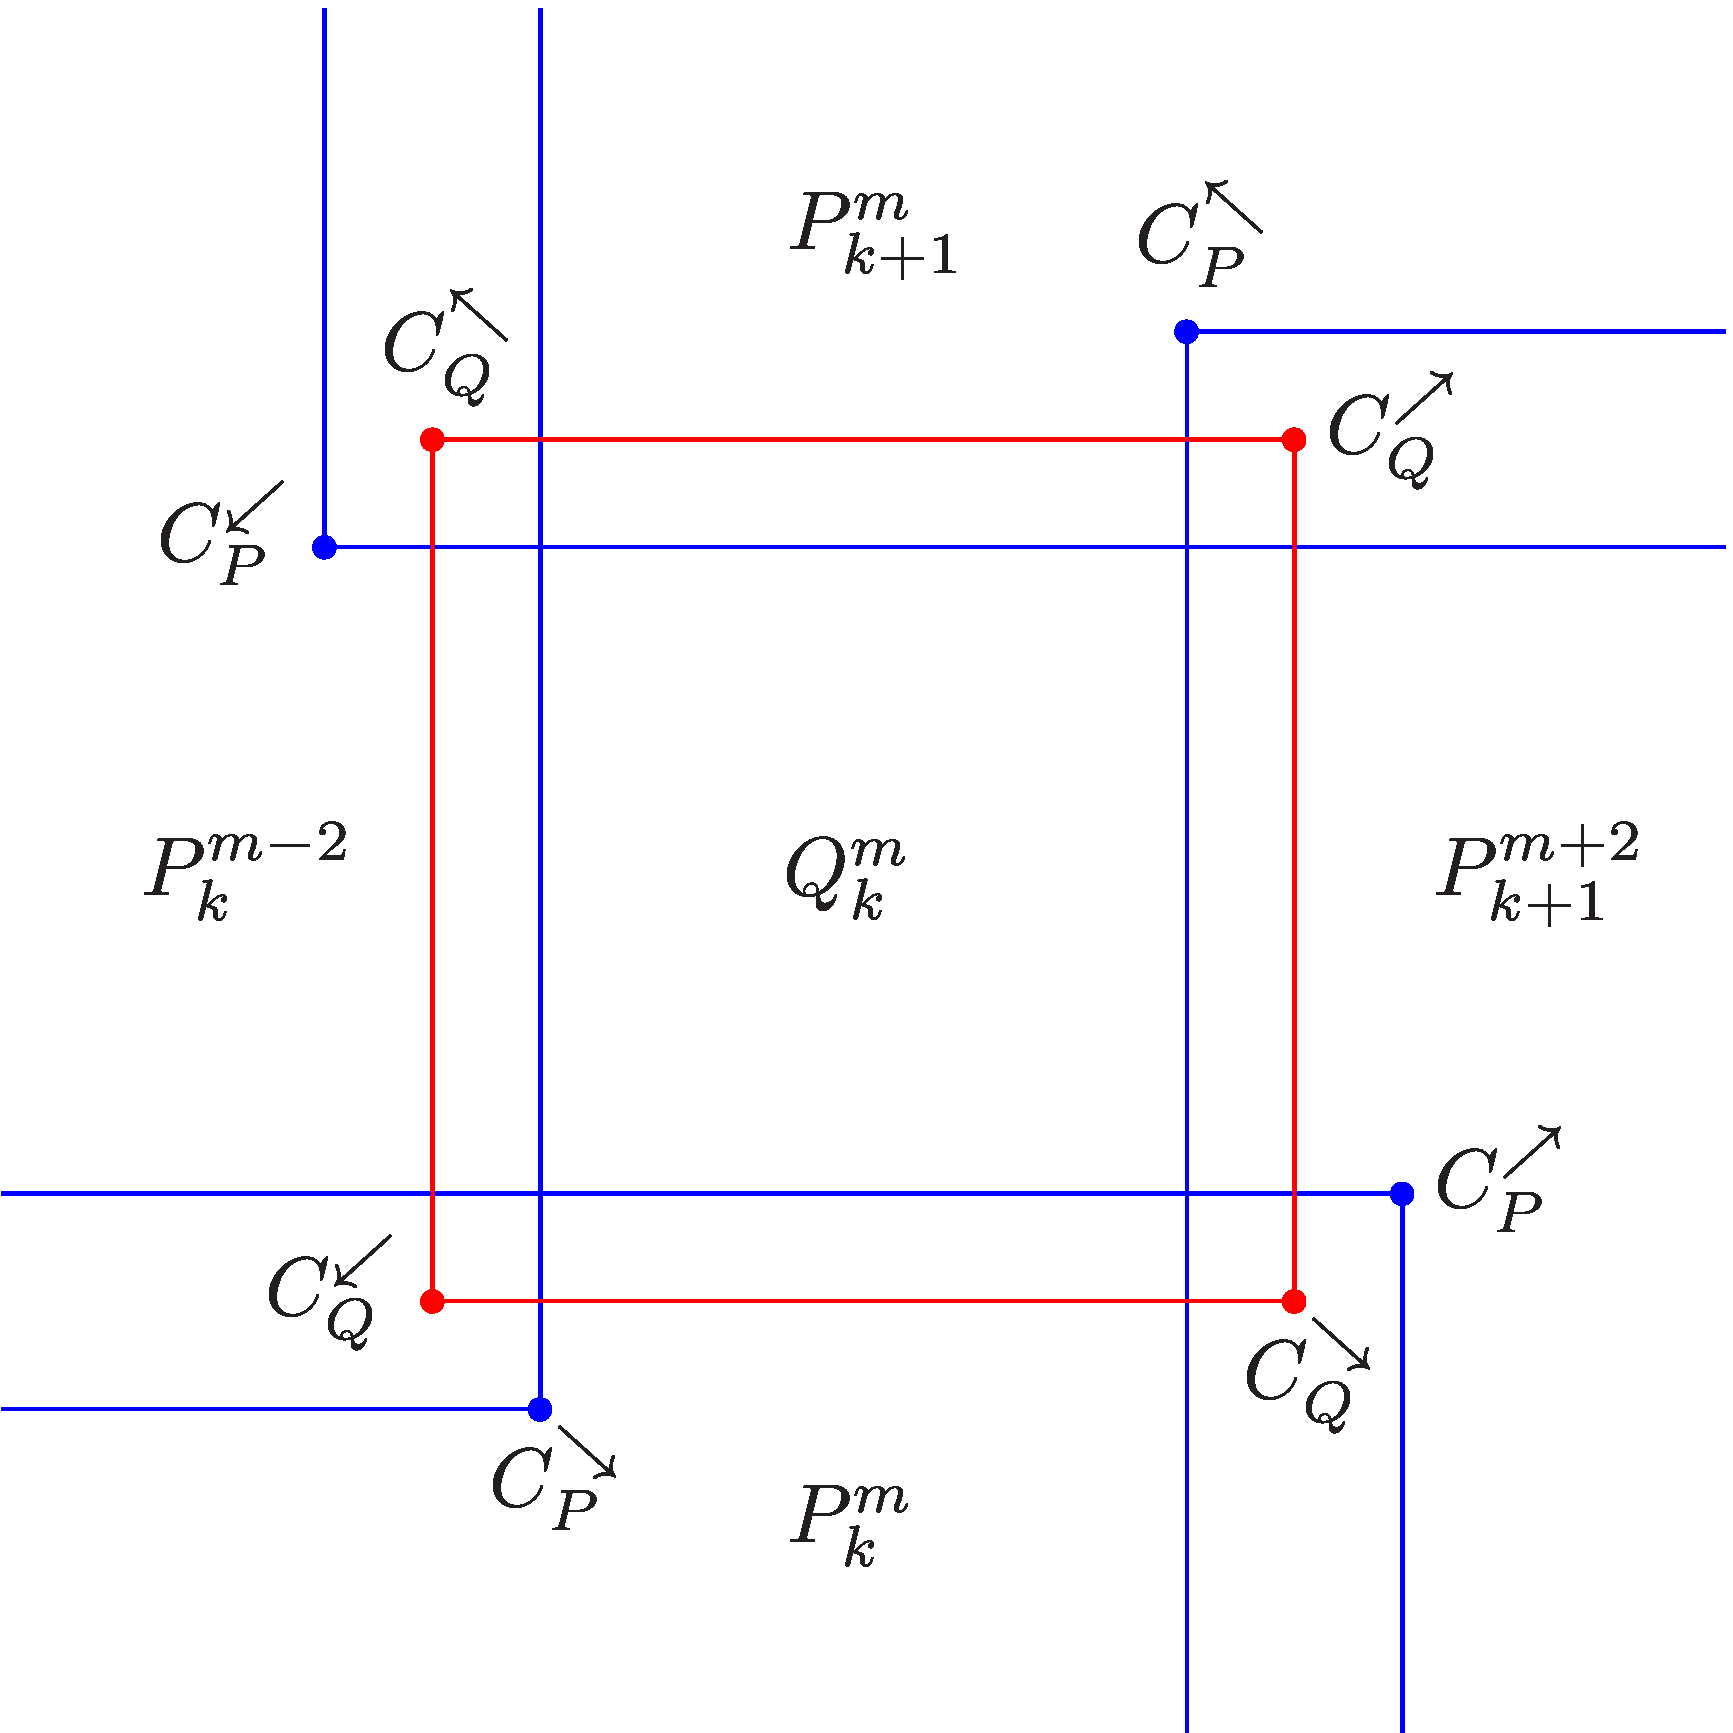
\includegraphics[width=.4 \textwidth]{../Figures/7/7.9a/result.png}
		\label{fig:add.change.schema.a}
	}
	\subfloat[]{
		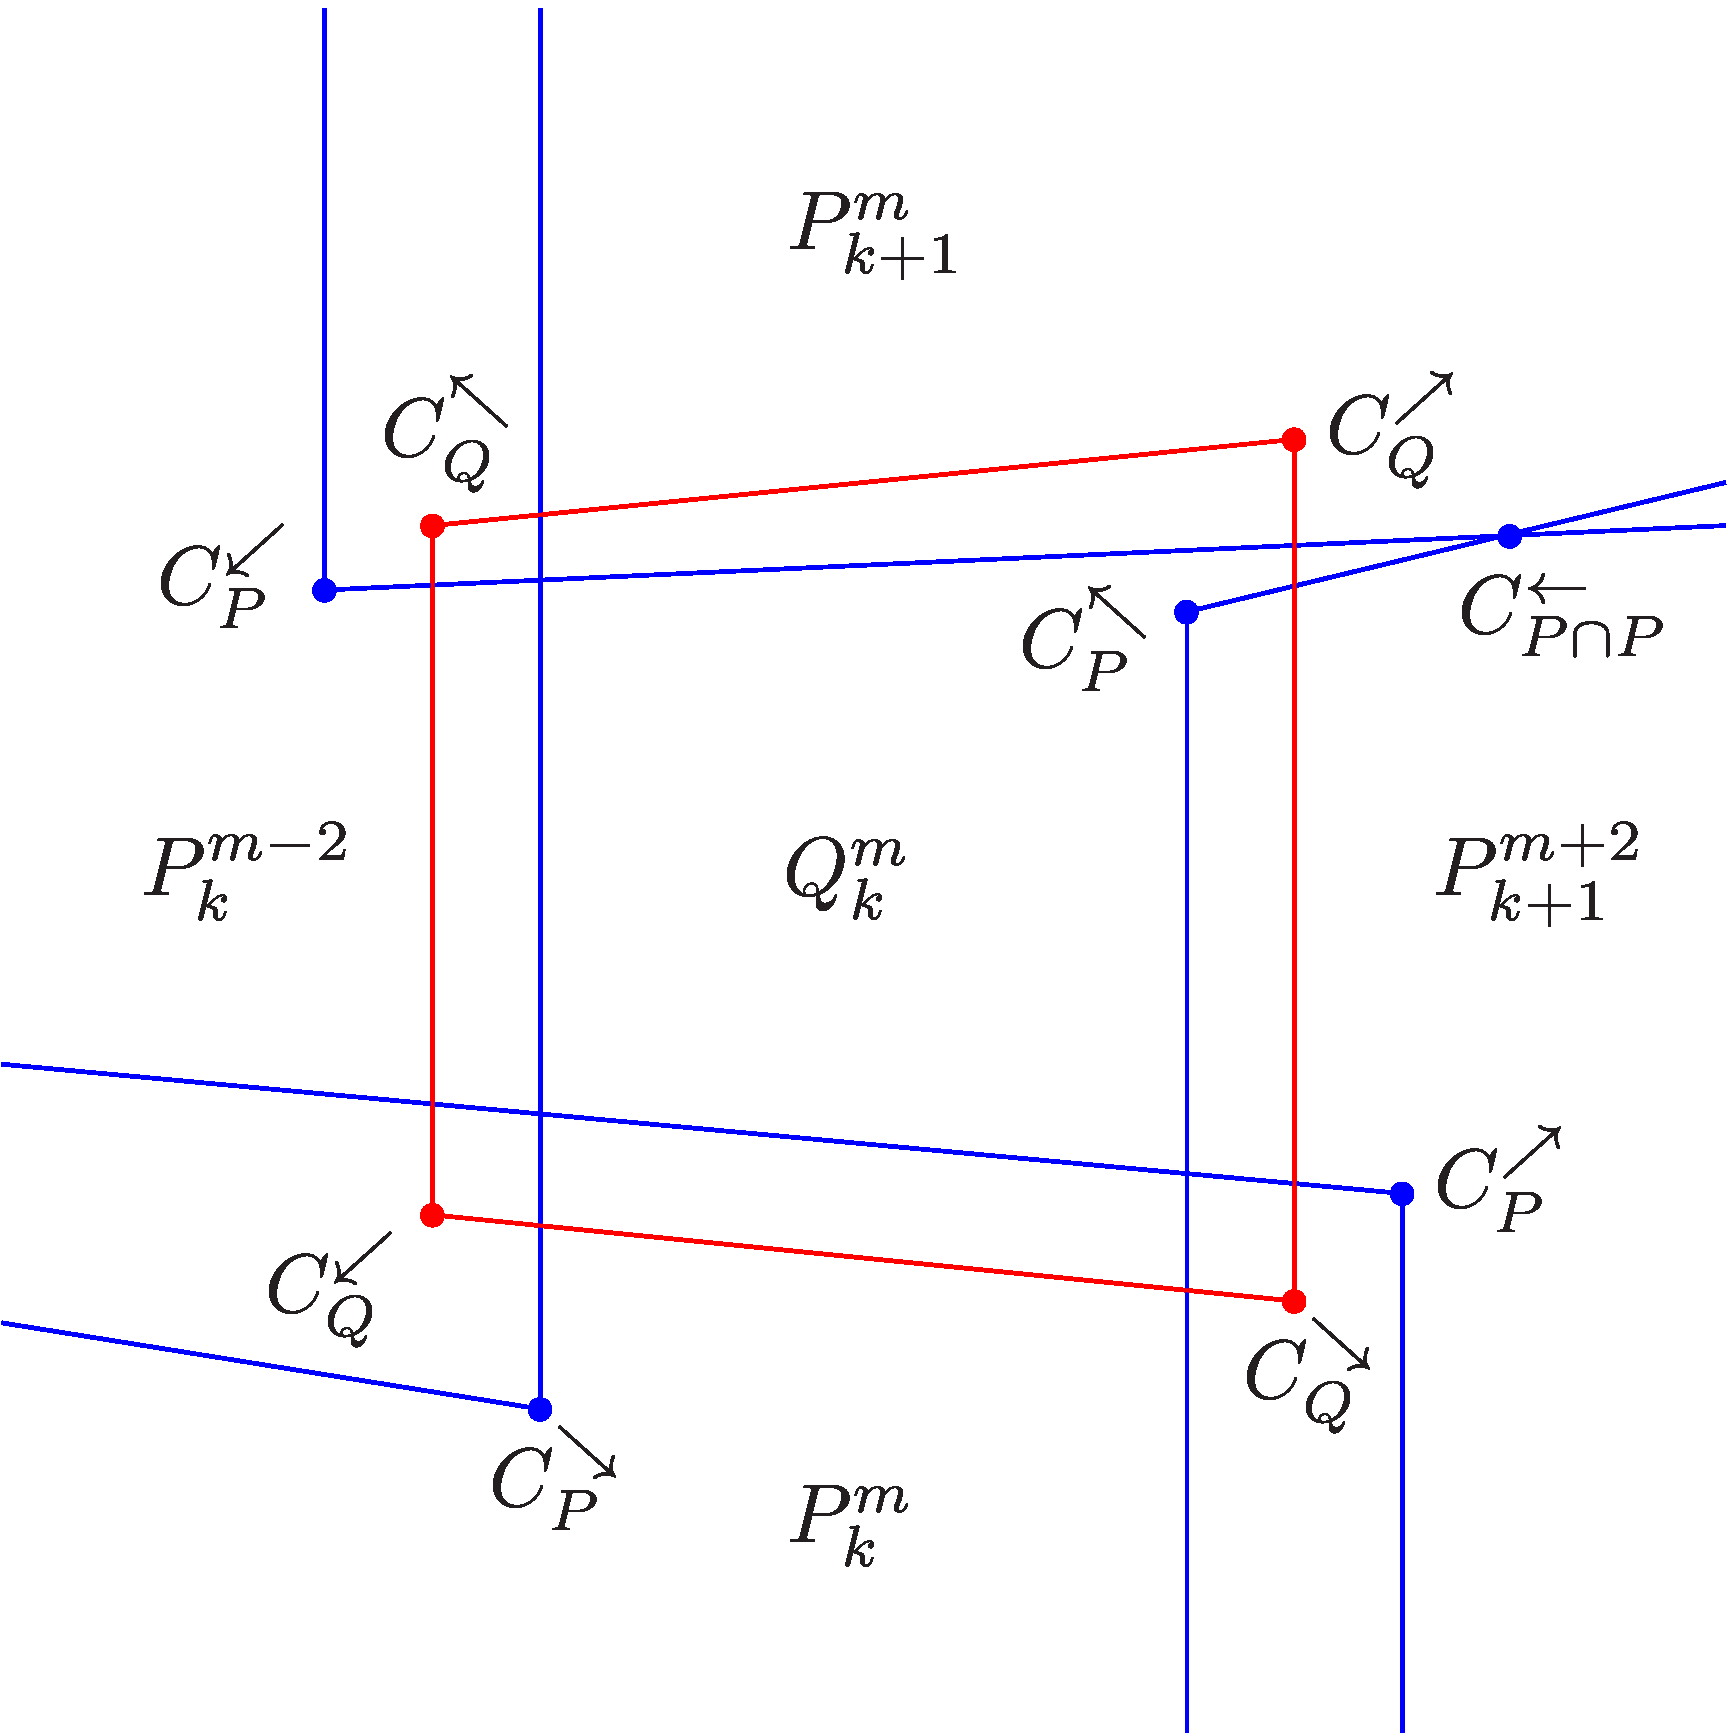
\includegraphics[width=.4 \textwidth]{../Figures/7/7.9b/result.png}
		\label{fig:add.change.schema.b}
	} \\
	\subfloat[]{
		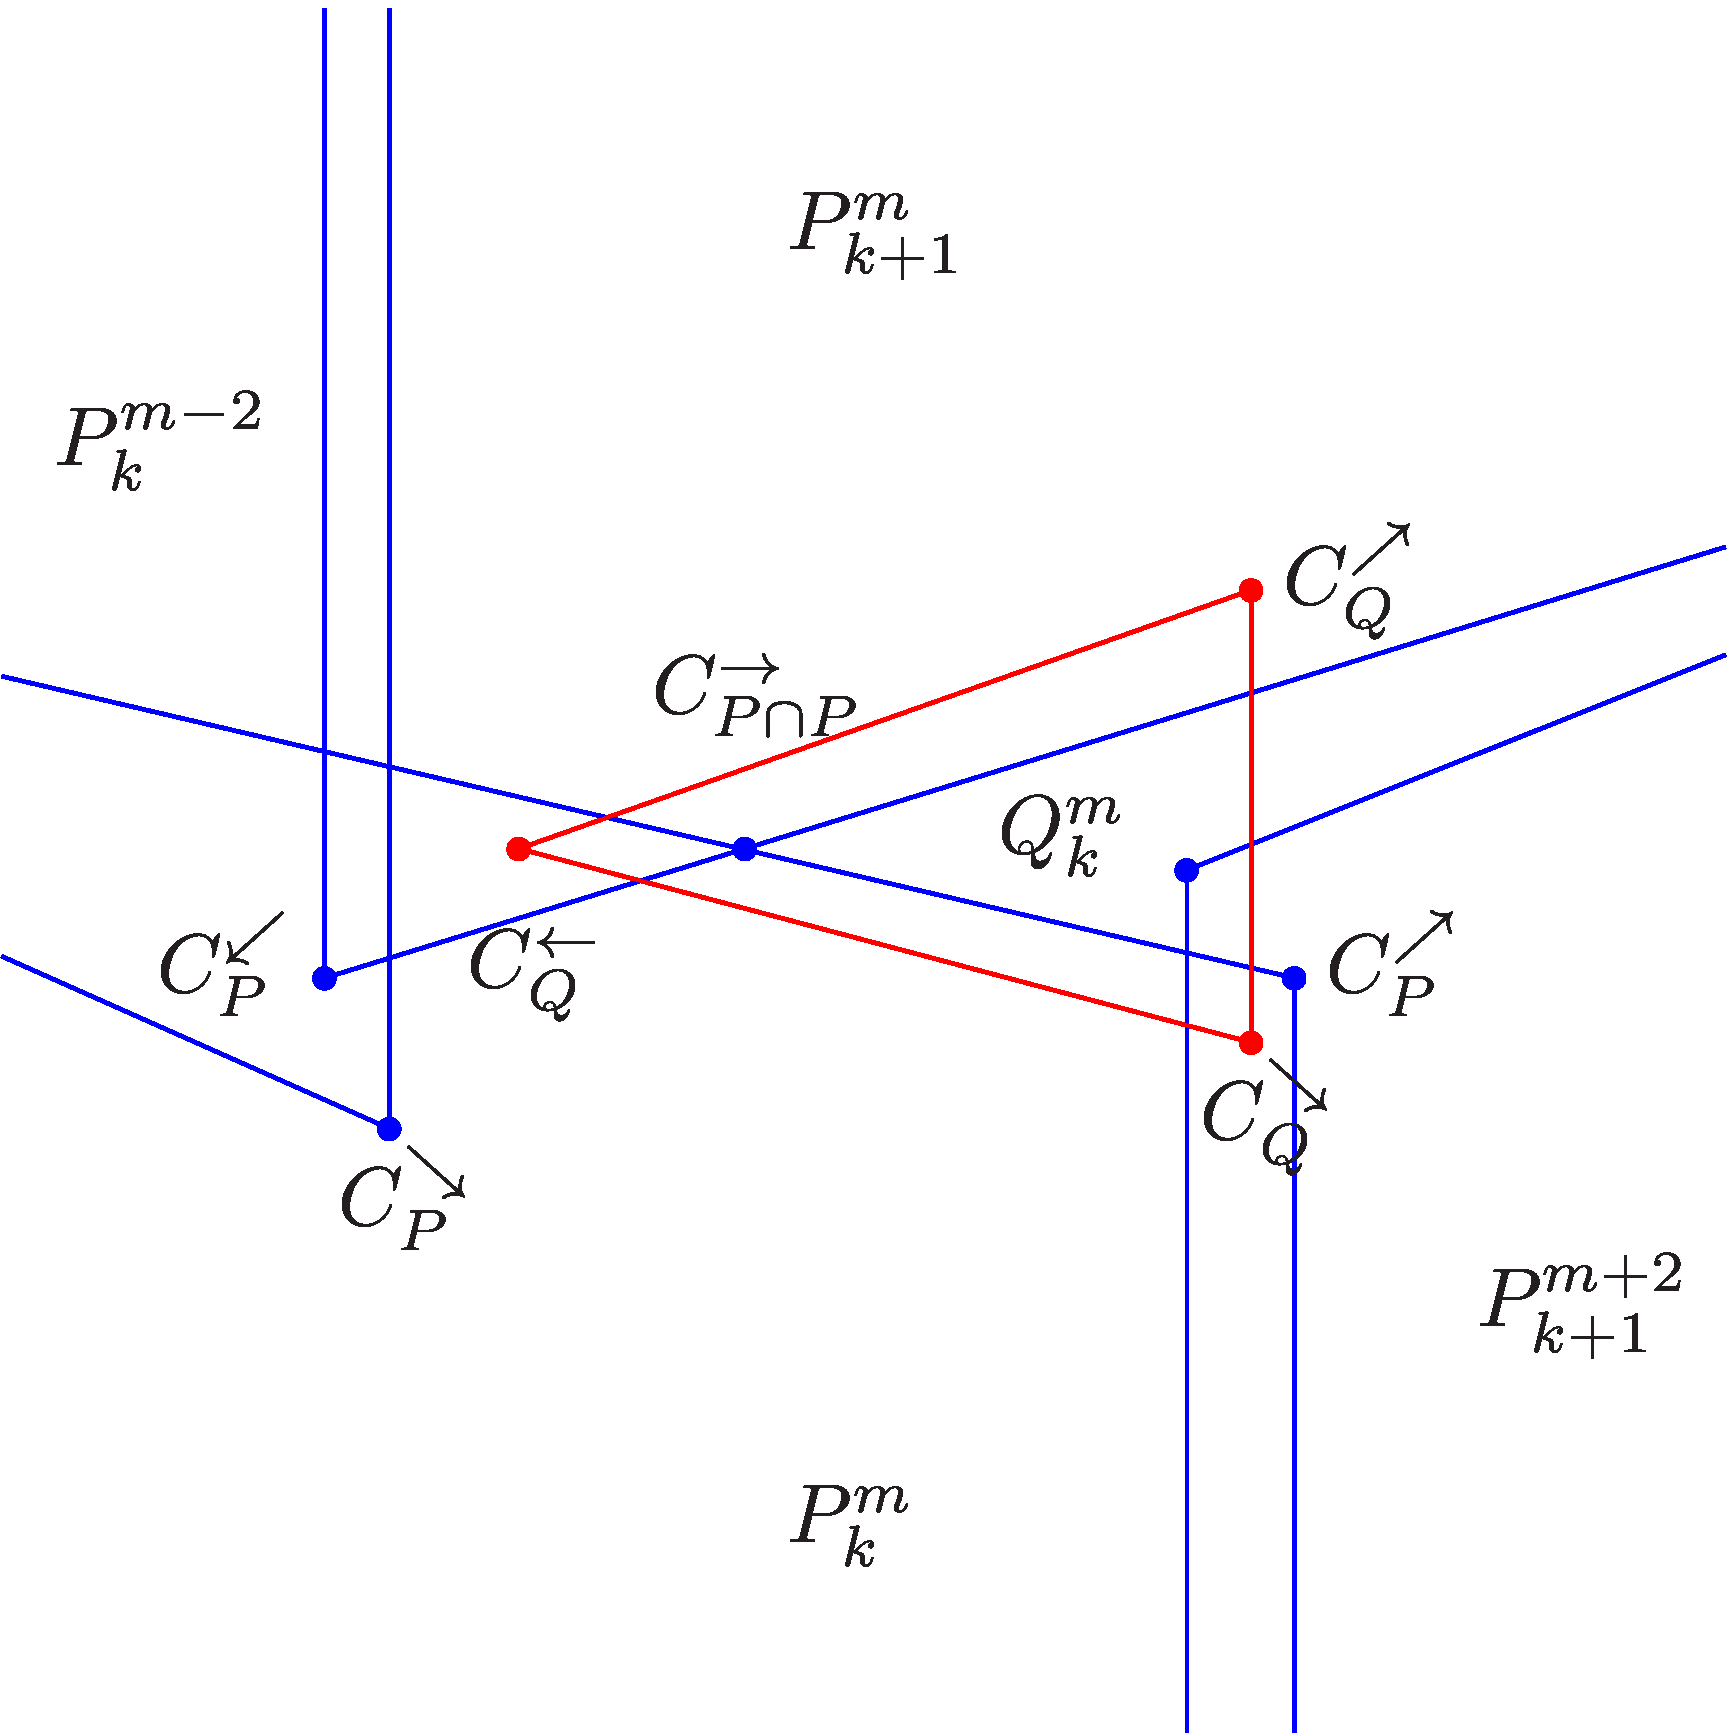
\includegraphics[width=.4 \textwidth]{../Figures/7/7.9c/result.png}
		\label{fig:add.change.schema.c}
	}
	\subfloat[]{
		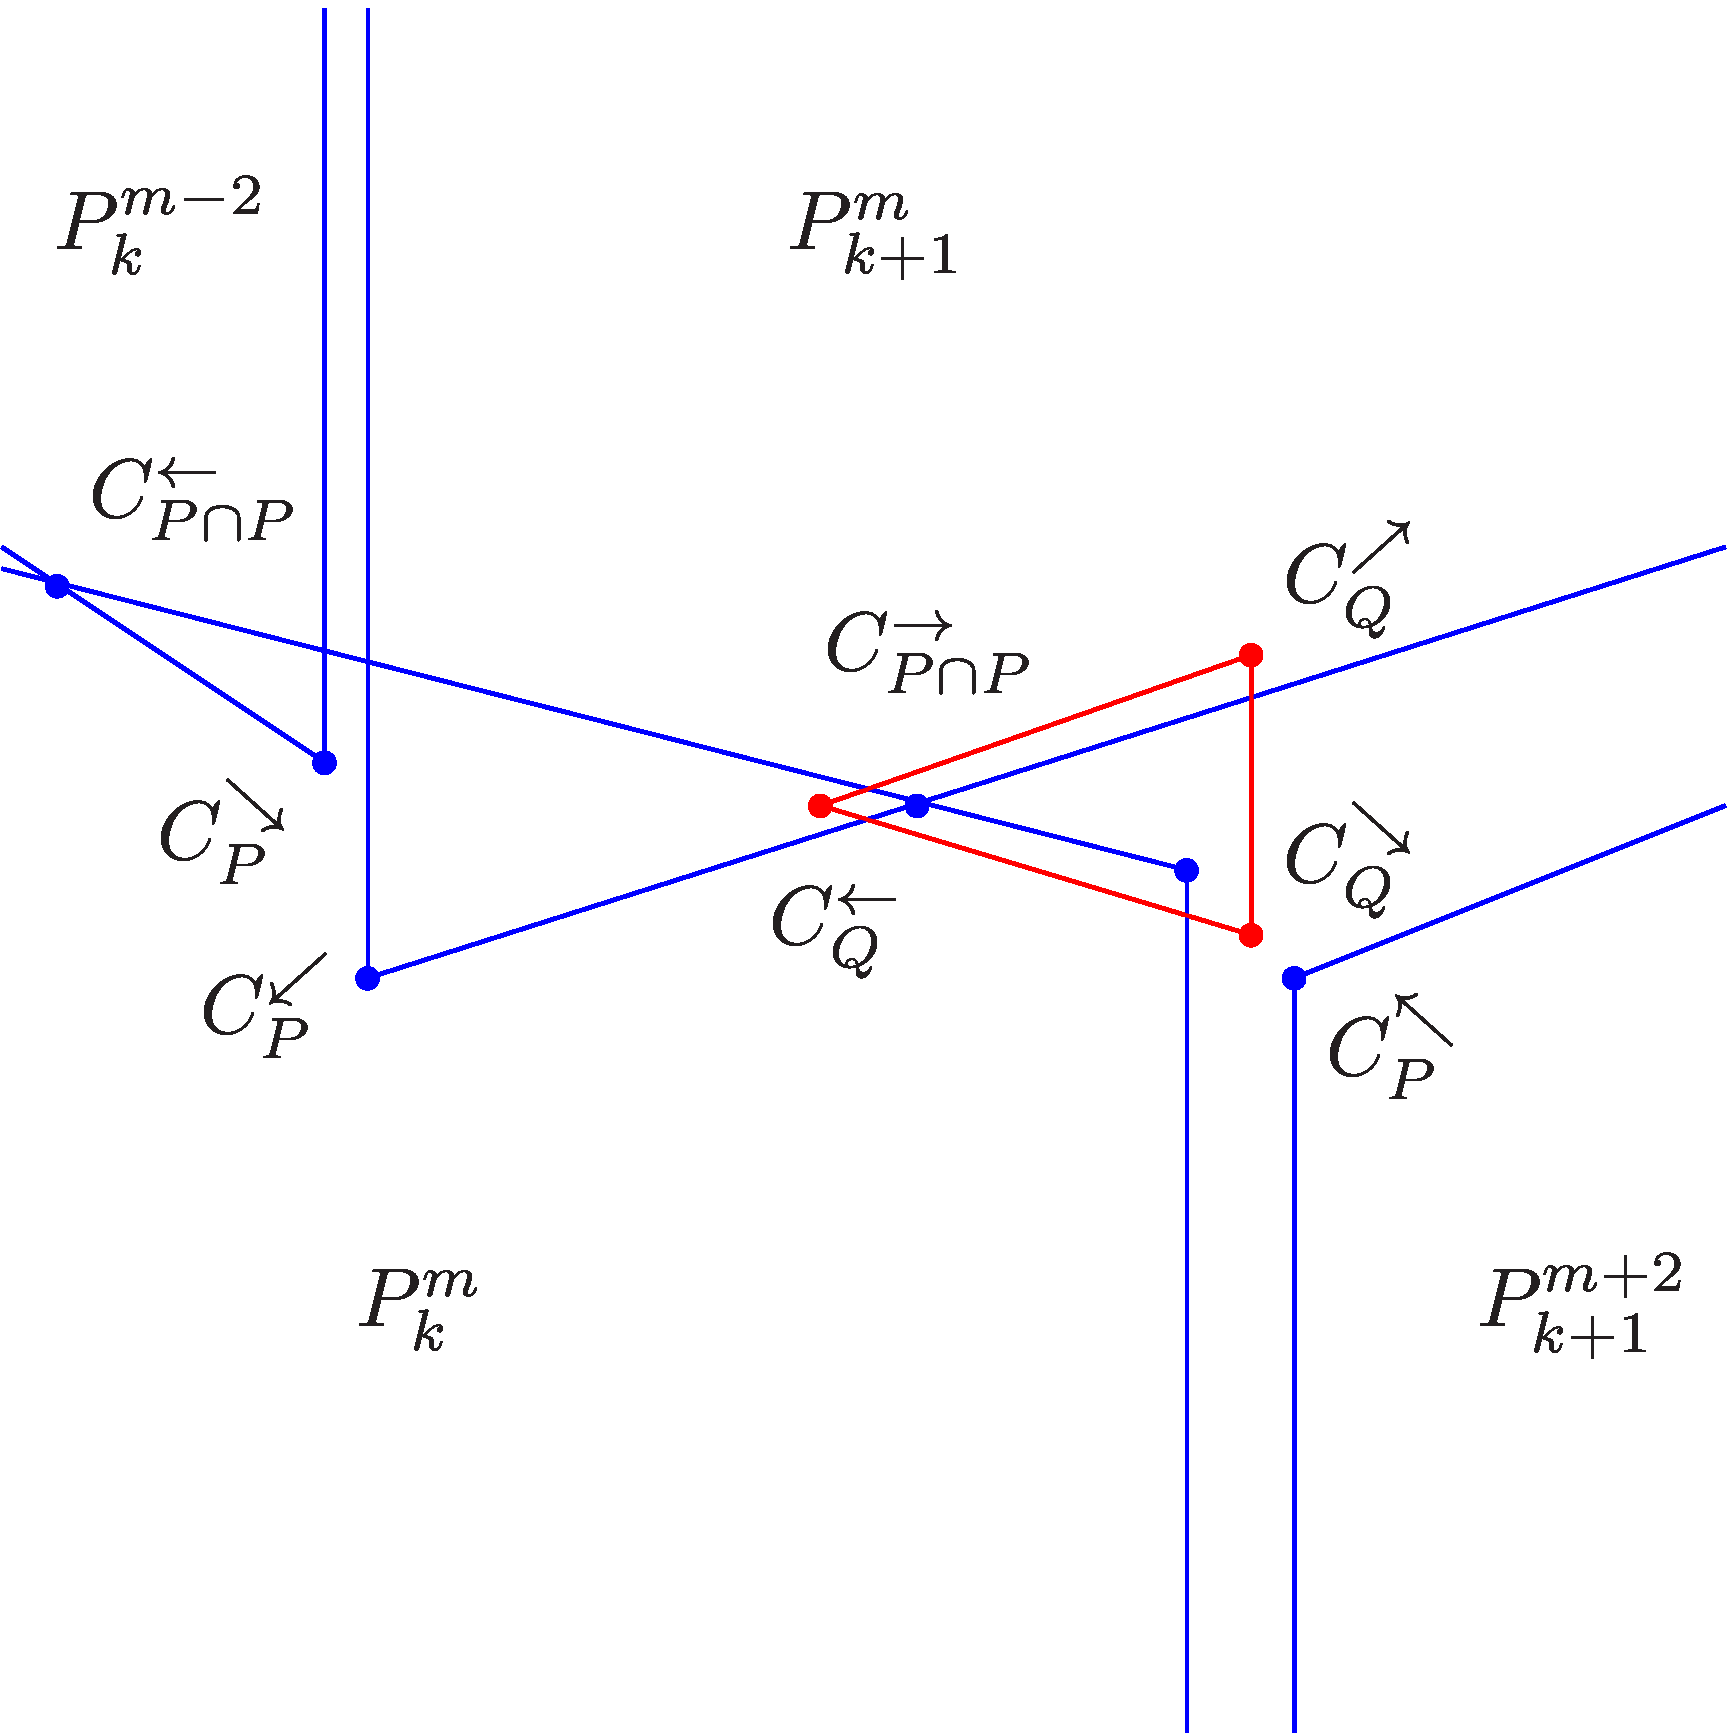
\includegraphics[width=.4 \textwidth]{../Figures/7/7.9d/result.png}
		\label{fig:add.change.schema.d}
	} \\
	\subfloat[]{
		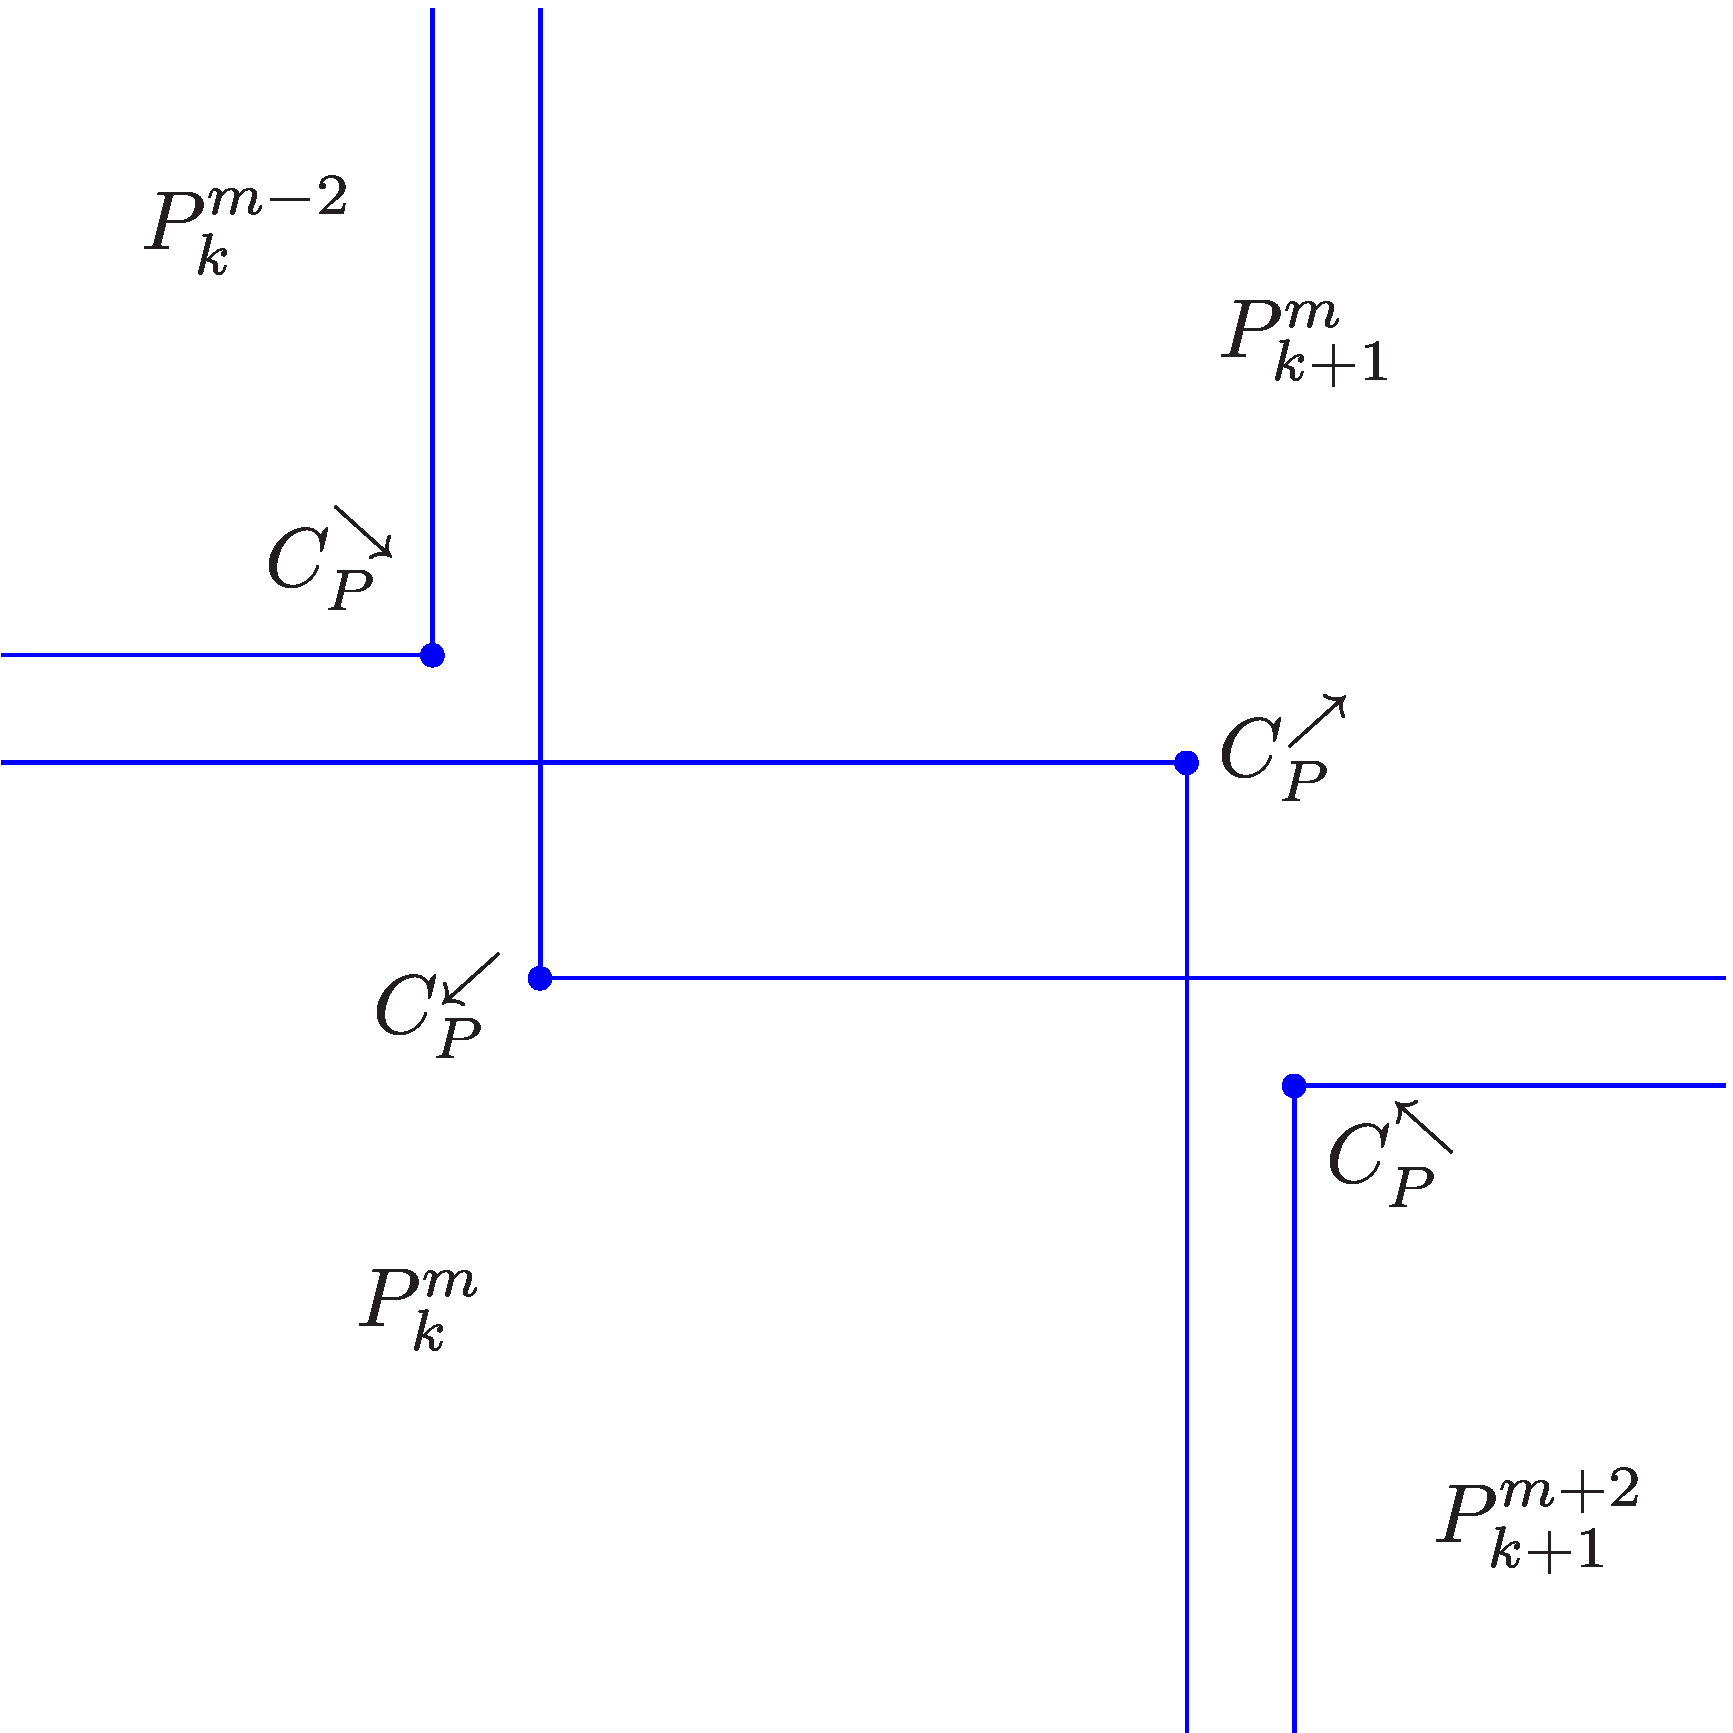
\includegraphics[width=.4 \textwidth]{../Figures/7/7.9e/result.png}
		\label{fig:add.change.schema.e}
	}
	\caption[Schematics of the boundaries of parameter regions associated with different symbolic sequences during the transition of the archetypal model to increasing branches]{
		Schematics of the boundaries of parameter regions associated with different symbolic sequences during the transition of the archetypal model to increasing branches.
		The boundaries of ``type A'' parameter regions are shown in blue while the boundaries of ``type B'' parameter regions are shown in red.
		Significant points where boundaries meet or cross are marked with dots.
	}
	\label{fig:add.change.schema}
\end{figure}

\Cref{fig:add.change.schema} shows multiple schematics that are used in this section to summarize all changes.
All schematics show some boundaries of the ``type A'' parameter regions $P^m_k, P^{m-2}_{k-1}, P^m_{k+1},$ and $P^{m+2}_{k+1}$ and all boundaries of the ``type B'' parameter region $Q^m_k$.
The ``type B'' parameter region is in-between all the ``type A'' parameter regions in the beginning.
This is shown in \Cref{fig:add.change.schema.a}.
The corners of the parameter regions are marked as follows.
The upper right corner of the ``type B'' parameter region in the middle is marked with the point $C_Q^\nearrow$.
Similarly, the lower right corner is marked with the point $C_Q^\searrow$ and the remaining corners with the points $C_Q^\nwarrow$ and $C_Q^\nwarrow$.
The corners of the ``type A'' parameter regions are marked analogously with $C_P^\nearrow, C_P^\searrow, C_P^\nwarrow,$ and $C_P^\swarrow$.
But here, the corners belong to different parameter regions.

The changes are summarized in the order they happen to the parameter regions that are considered in the previous sections.
This order might differ for different parameter regions.

First, the upper left corner $C_Q^\nwarrow$ of the lower right ``type A'' parameter region $P^{m+2}_{k+1}$ moves down and crosses the lower boundary of the upper right ``type A'' parameter region $P^m_{k+1}$.
This is visible in \Cref{fig:add.change.schema.b}.
The point where the two boundaries of the horizontally neighboring ``type A'' parameter regions cross is marked as $C_{P \cap P}^\leftarrow$ because this point is now the only left corner point of the overlapping parameter region $P^{m+2}_{k+1} \cap P^{m}_{k+1}$.
For higher values of $b_L$, the point $C_Q^\nwarrow$ moves further down which causes the point where the boundaries cross to move right.
In \Cref{fig:add.change.schema.c}, this crossing point is not visible anymore, since it moved out of the domain of the picture.
In \Cref{fig:add.change.schema.d}, it is visible again, but on the left side of the schema.
Strictly speaking, this is not the same point but the left boundary of the overlapping parameter region $P^m_k \cap P^{m-2}_{k}$.
This point then collides with the corner point $C_P^\nearrow$ which then causes the two ``type A'' parameter regions to not overlap anymore.
This final scenario can be seen in \Cref{fig:add.change.schema.e}.
In the spaces that opened up between the vertically neighboring ``type A'' parameter regions, there are big hybrid parameter regions $\left[P^{m+2}_{k+1} \mid P^{m}_{k+1}\right]$ and $\left[P^m_k \mid P^{m-2}_k\right]$, respectively.
The hybrid parameter regions are not shown in the schematics but while the overlapping parameter regions have only three boundaries, they too only have three boundaries and are bounded to the right only by one codimension-2 point.
At this point, their upper and lower boundaries meet.

As we can see in the schematics, this change starts first and finishes last.
While the described process occurs, another change starts happening.
The points $C_P^\searrow$ and $C_Q^\nearrow$ move down while the points $C_Q\searrow$ and $C_P^\nearrow$ move up.
As soon as the point $C_P^\swarrow$ crosses the upper boundary of $P^m_k$, the ``type A'' parameter regions $P^m_k$ and $P^m_{k+1}$ start to overlap.
This overlapping region is bounded to the right only by the point where the horizontal boundaries of those two parameter regions cross.
This point is marked as $C_{P \cap P}^\rightarrow$ in \Cref{fig:add.change.schema.c}.
Also at some parameter values the corner points $C_Q^\nwarrow$ and $C_Q^\searrow$ of the ``type B'' parameter region $Q^m_k$ in the middle collide.
This creates a codimension-2 point that bounds the parameter region $Q^m_k$ to the left, hence it is marked as $C_Q^\leftarrow$.
Both these newly created corner points move right, as can be seen in \Cref{fig:add.change.schema.d}.
Finally, the corner point $C_{P \cap P}^\rightarrow$ collides with the corner point $C_P^\nearrow$ and the two horizontal boundaries of the ``type A'' parameter regions stop crossing.
The overlapping parameter region $P^m_k \cap P^m_{k+1}$ is now bounded by four boundaries, as can be seen in \Cref{fig:add.change.schema.e}.
And the corner point $C_Q^\leftarrow$ crosses the right boundary of the ``type B'' parameter region, destroying the ``type B'' parameter region.

While that change is happening, one more change takes place.
This change does not happen by two boundaries crossing at one point like the last two changes.
Instead, the numeric evidence suggests that it happens at once.
The corner point $C_P^\nwarrow$ crosses the right boundary of $P^m_k$ at the same time, the lower right corner point of $P^{m}_{k}$ which is not pictured here crosses the left boundary of $P^{m+2}_{k+1}$.
This lower corner point is not pictured, but the lower right corner point of $P^{m-2}_k$ is pictured and marked as $C_P^\searrow$.
Here, the equivalent happens for the horizontally neighboring ``type A'' parameter regions $P^{m-2}_k$ and $P^m_{k+1}$.
In \Cref{fig:add.change.schema.c}, the horizontally neighboring ``type A'' parameter regions overlap and in \Cref{fig:add.change.schema.d}, the parameter regions do not overlap.
Instead, there is now space in-between the horizontally neighboring ``type A'' parameter regions.
In this space there now is a big hybrid parameter region and \gls{pal} structures, similar to the vertically neighboring ``type A'' parameter regions.

\subsubsection{Observations}

The local minima on branches $f_\A$ and $f_\C$ seem to be important for the ``type B'' parameter regions.
That means, parameter regions with coexisting asymmetrical cycles with the \textbf{same} period.
At the same time, these minima seem to prevent period-adding structures.
It will be proven next that ``type B'' parameter regions are impossible with only increasing branches.

\begin{lemma}[Number and Positions of Points of two Cycles on an Increasing Branch]
	Let $f_\X$ be an increasing branch of some model function $f$.
	If two cycles $\sigma_1$ and $\sigma_b$ have points on this branch, there are two possibilities for the relative number of points and relative position of the points.
	\begin{enumerate}
		\item Both cycles have the same number of points on the branch $f_\X$.
		      Let the first point of $\sigma_1$ be to the left of the first point of $\sigma_2$ on this branch w.l.o.g.
		      Then the last point of $\sigma_1$ is also to the left of the last point of $\sigma_2$ on this branch.
		      \Cref{fig:add.change.increasing.a} illustrates this case.
		\item One cycle has one more point on the branch $f_\X$.
		      Let $\sigma_1$ be the cycle with more points on this branch w.l.o.g.
		      Then the first point of $\sigma_1$ is to the left of the first point of $\sigma_2$ on this branch and the last point of $\sigma_1$ is to the right of the last point of $\sigma_2$ on this branch.
		      \Cref{fig:add.change.increasing.b} illustrates this case.
	\end{enumerate}
	\label{lemma:add.num.pos.points.increasing}
\end{lemma}

\begin{figure}
	\centering
	\subfloat[Same number of points]{
		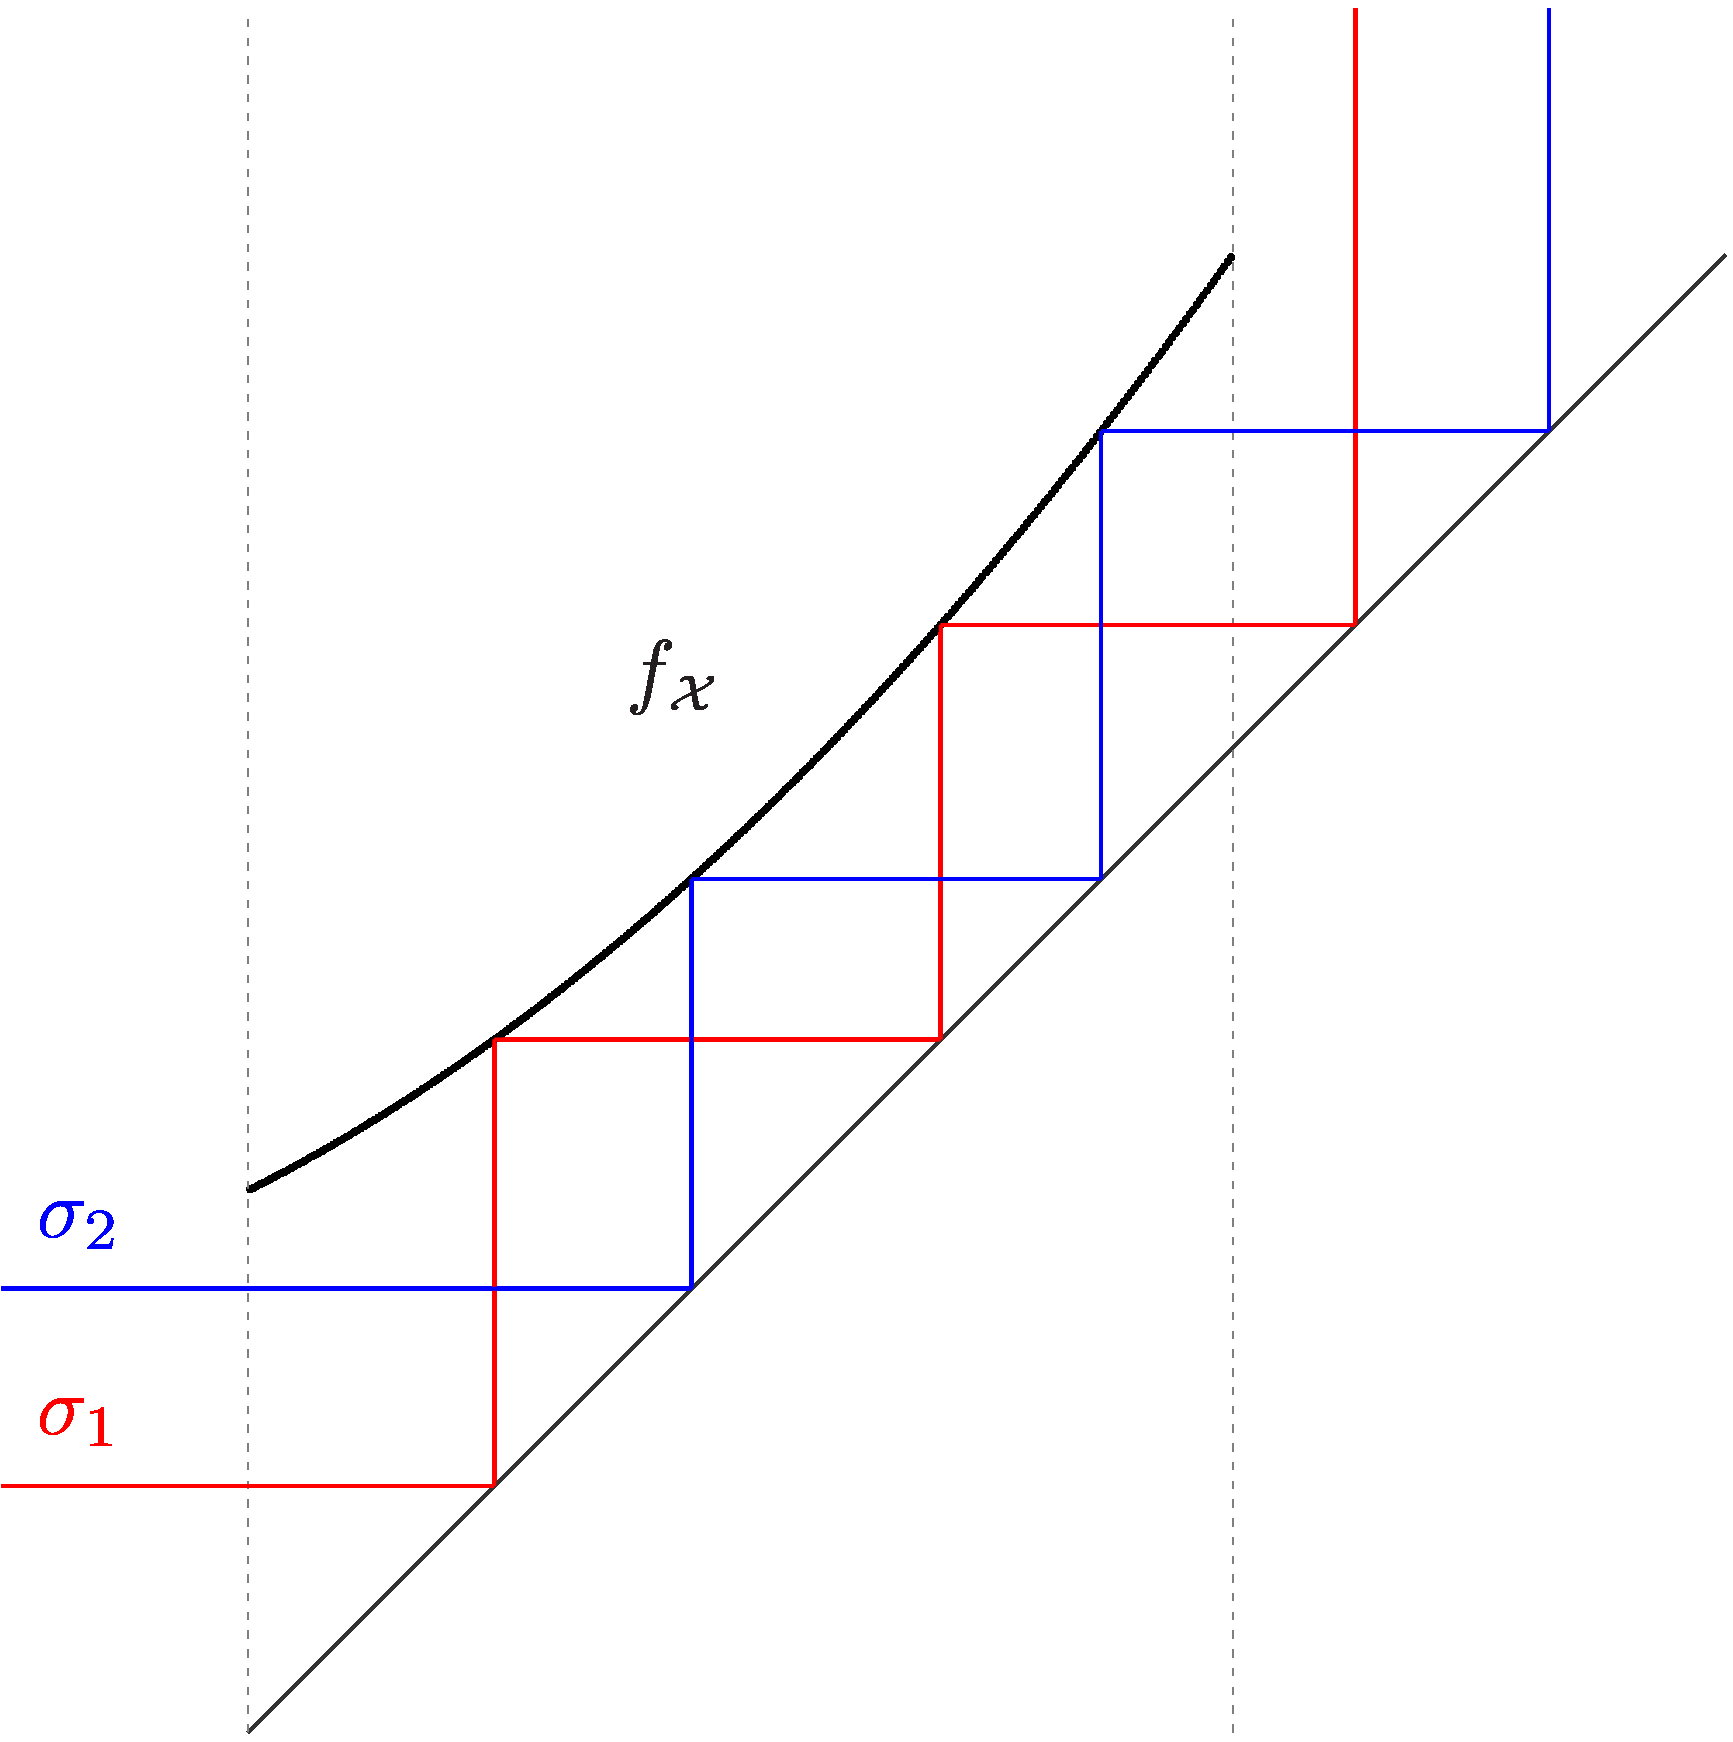
\includegraphics[width=.35 \textwidth]{../Figures/7/7.10a/result.png}
		\label{fig:add.change.increasing.a}
	} \quad
	\subfloat[Number of points differing by one]{
		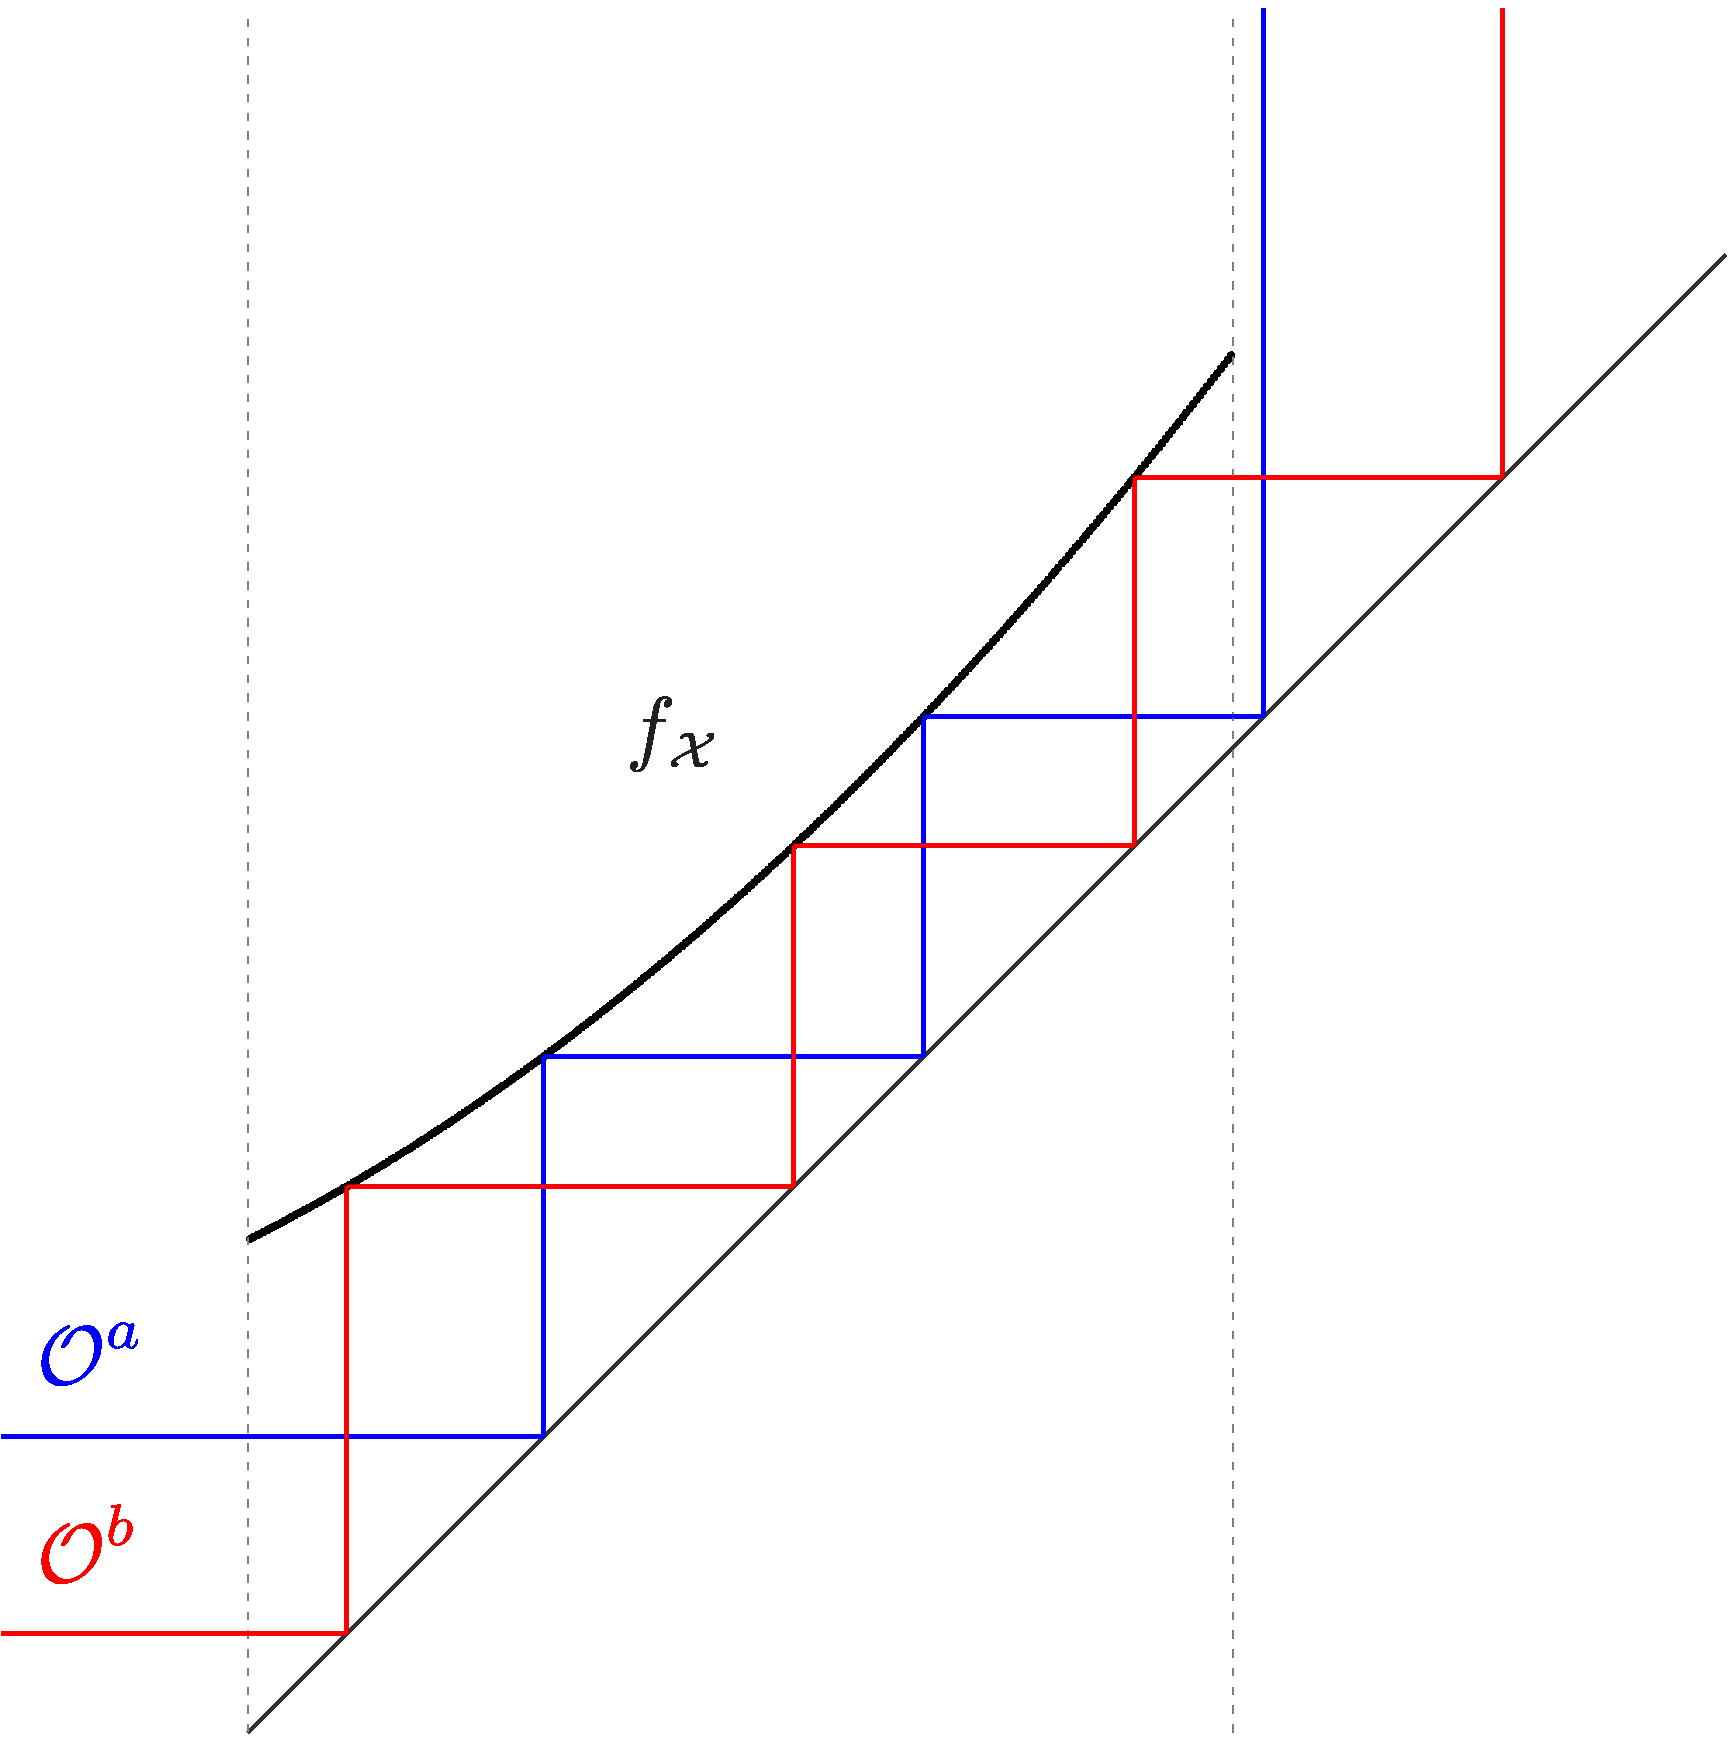
\includegraphics[width=.35 \textwidth]{../Figures/7/7.10b/result.png}
		\label{fig:add.change.increasing.b}
	}
	\caption[Illustration of the relative number and positions of the points of two cycles on an increasing branch]{
		Illustration of the relative number and positions of the points of two cycles on an increasing branch.
		Both figures show a function branch $f_\X$ and parts of two cycles, $\sigma_1$ shown in red and $\sigma_2$ shown in blue.
		(a) shows the case where both cycles have the same number of points on the branch $f_\X$ and the first point of $\sigma_1$ is to the left of the first point of $\sigma_2$ on this branch.
		(a) shows the case where the cycle $\sigma_1$ has one point more on the branch $f_\X$ than $\sigma_2$ and the first point of $\sigma_1$ is to the left of the first point of $\sigma_2$ on this branch.
	}
	\label{fig:add.change.increasing}
\end{figure}

\begin{theorem}[No ``Type B'' Parameter Regions with only Increasing Branches]
	The ``type B'' parameter regions are not possible in the increasing archetypal model.
	The minima on the branches $f_\A$ and $f_\C$ are essential for the bifurcation structure.
\end{theorem}

\begin{proof} \phantom{x} \\
	Let's assume that all branches of the archetypal model $f_\A, f_\B, f_\C,$ and $f_\D$ are increasing.
	And let $\sigma_1$ and $\sigma_2$ be ``type B'' twin cycles.
	The following conditions are true for such cycles.
	\begin{subequations}
		\begin{align}
			|\sigma_1|_\A - 1 & = |\sigma_2|_\A \label{equ:add.change.conseq.sigmaA} \\
			|\sigma_1|_\B + 1 & = |\sigma_2|_\B \label{equ:add.change.conseq.sigmaB} \\
			|\sigma_1|_\C + 1 & = |\sigma_2|_\C \label{equ:add.change.conseq.sigmaC} \\
			|\sigma_1|_\D - 1 & = |\sigma_2|_\D \label{equ:add.change.conseq.sigmaD}
		\end{align}
	\end{subequations}

	For \Cref{equ:add.change.conseq.sigmaA} to hold, the first point of  $\sigma_1$ needs to be to the left of first point of  $\sigma_2$ on the branch $f_\A$, because  $\sigma_1$ has one point more on this branch than  $\sigma_2$ and this branch is increasing.
	At the same time, the last point of  $\sigma_1$ must be to the right of the last point of  $\sigma_2$ on this branch.

	The order of the first points on the next branch, $f_\B$, is the same as for the last points on the branch $f_\A$.
	So the first point of  $\sigma_2$ is to the left of the first point of  $\sigma_1$ on this branch.
	For \Cref{equ:add.change.conseq.sigmaB} to hold, the last point of  $\sigma_2$ must be to the right of the last point of  $\sigma_1$ on this branch per the same logic as before.

	The order of the first points on the next branch, $f_\C$, is the same as for the last points on the branch $f_\B$.
	So the first point of  $\sigma_1$ is to the left of the first point of  $\sigma_2$ on this branch.
	This is a contradiction, since the first point of  $\sigma_1$ on the branch $f_\A$ is also to the left of the first point of  $\sigma_2$ on that branch.
	This violates the symmetry.
	Also, \Cref{equ:add.change.conseq.sigmaC} cannot be fulfilled if the first point of  $\sigma_1$ is to the left of the first point of  $\sigma_2$ on the branch $f_\C$, since the first point of  with more points, $\sigma_2$ in this case, on the branch must be to the left of the first point of the other cycle on that branch if the branch is increasing.

	\hfill $\blacksquare$
\end{proof}


\clearpage
\section{The Period-adding-like Structures}
\label{sec:add.add}

Now that we know, how the period-adding-like structures develop, we will describe them in this section.

\subsection{Description of the Structures in the Increasing Archetypal Model}
\label{sec:add.add.like}

\hl{
	The first step in the description of the \gls{pal} structures is plotting a 2D scan of the periods of such a structure.
}
Here, $b_L$ \hl{is changed} to $0.8$, and $a_L$ and $g_R\left(\frac{1}{2}\right)$ \hl{are kept as described before}, because the \gls{pal} structures are more pronounced at these parameter values.
\Cref{fig:add.add.like} shows a 2D period scan with these parameters at a corner of the space between chains.
Here, the parameter region $P^{12}_2$ is in the lower left corner and the parameter region $P^{12}_3$ of the same chain is in the upper right corner.
In the lower right corner is the parameter region $P^{14}_3$.

\hl{Next, this section takes} a closer look at the horizontally \gls{pal} structures between the parameter regions $P^{14}_3$ and $P^{12}_3$.
\hl{After that, it examines} the vertically oriented \gls{pal} structures between the parameter regions $P^{12}_2$ and $P^{14}_3$.
And lastly, \hl{it examines} the complex looking structure in the corner between all three ``type A'' parameter regions.

\begin{figure}
	\centering
	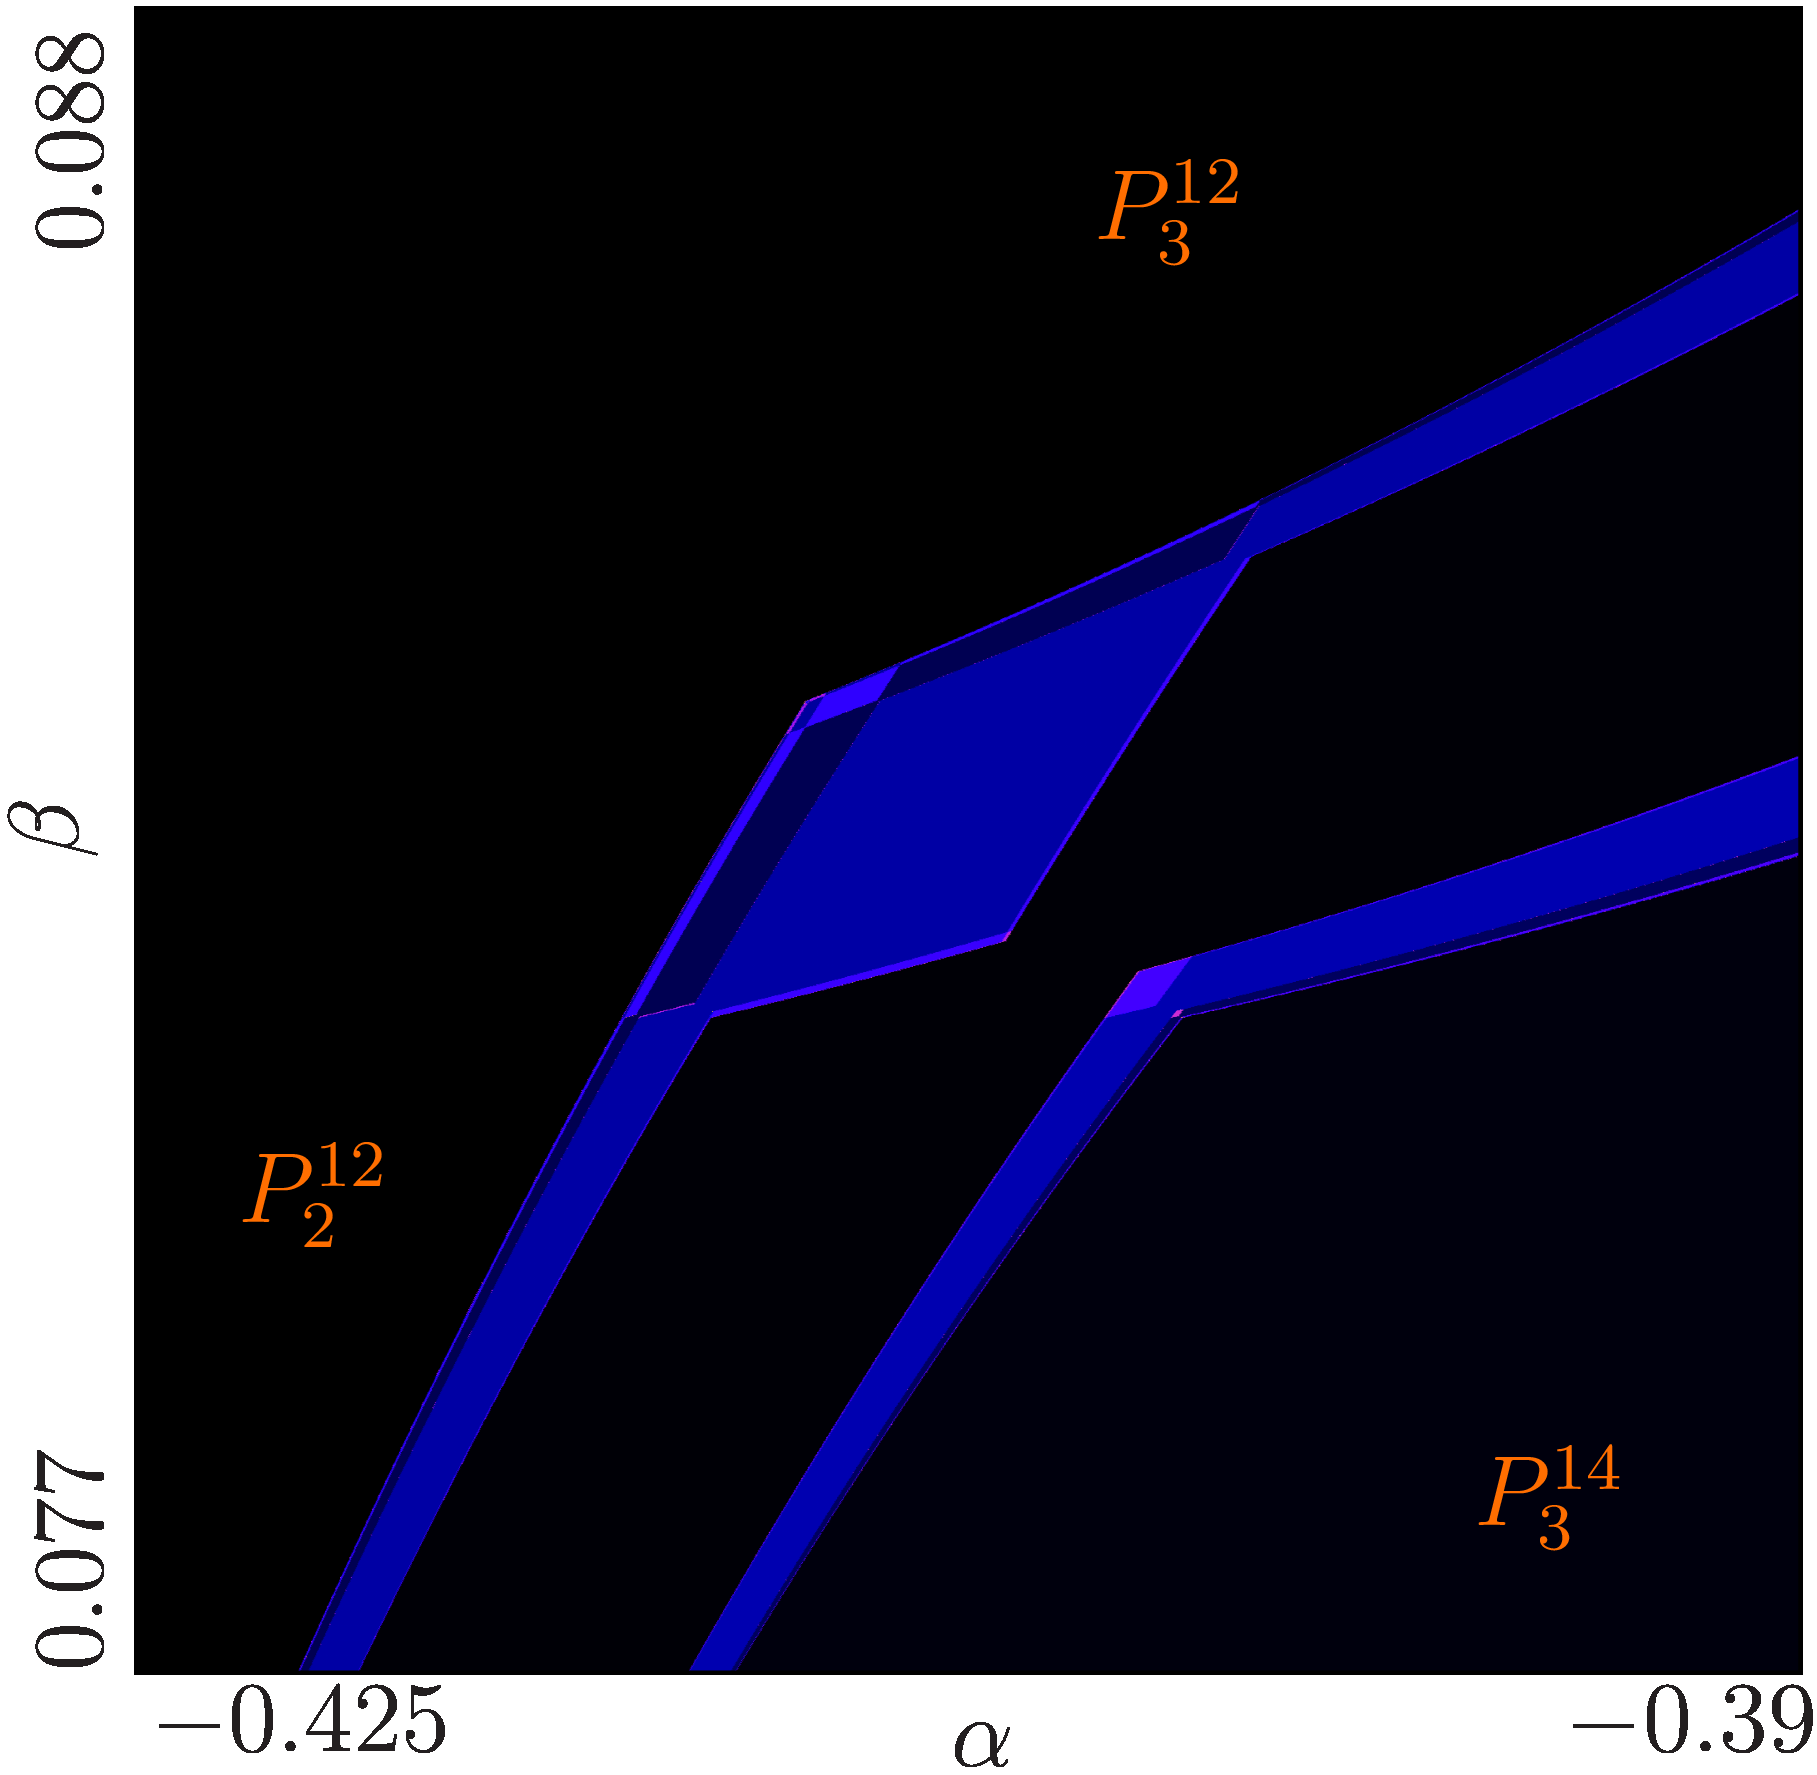
\includegraphics[width=.7 \textwidth]{../Figures/7/7.11/result.png}
	\caption[2D period scan of period-adding-like structures in the increasing archetypal model]{
		2D period scan of period-adding-like structures in the increasing archetypal model.
		The fixed parameters are $a_L = 1, b_L = 0.8,$ and $g_R\left(\frac{1}{2}\right) = \frac{1}{2} + \frac{1}{40}$.
		The parameters $\alpha = g_R\left(\frac{1}{4}\right)$ and $\beta = c_L$ are varied.
	}
	\label{fig:add.add.like}
\end{figure}

\subsubsection{Horizontal Period-adding-like Structures}

\Cref{fig:add.add.like.hor.2D} shows a 2D scan of the horizontally oriented \gls{pal} structures between the parameter regions $P^{14}_3$ and $P^{12}_3$.
We can see two \gls{pal} structures, one between the ``type A'' parameter region $P^{14}_3$ and the hybrid parameter region $\left[P^{14}_3 \mid P^{12}_3\right]$ and one in between the hybrid parameter region $\left[P^{14}_3 \mid P^{12}_3\right]$ and the ``type A'' parameter region $P^{12}_3$.
There is a red arrow in the 2D period scan that indicates the parameter range for the 1D period scan in \Cref{fig:add.add.like.hor.1D}.

Looking at the 1D period scan, one can see why the section is called \glsentrylong{pal}.
In the middle between the parameter regions associated with the periods $14$ and $13$, we would expect the most pronounced parameter region to be associated with the period $27$.
Instead, the most pronounced parameter region in-between those parameter regions is associated with the period $40$.
And the most pronounced parameter region between this parameter region and the parameter region associated with the period $14$, has period $27$ where we would expect period $54$.
We can see that the periods do not add in our case.

\begin{figure}
	\centering
	\subfloat[2D period scan]{
		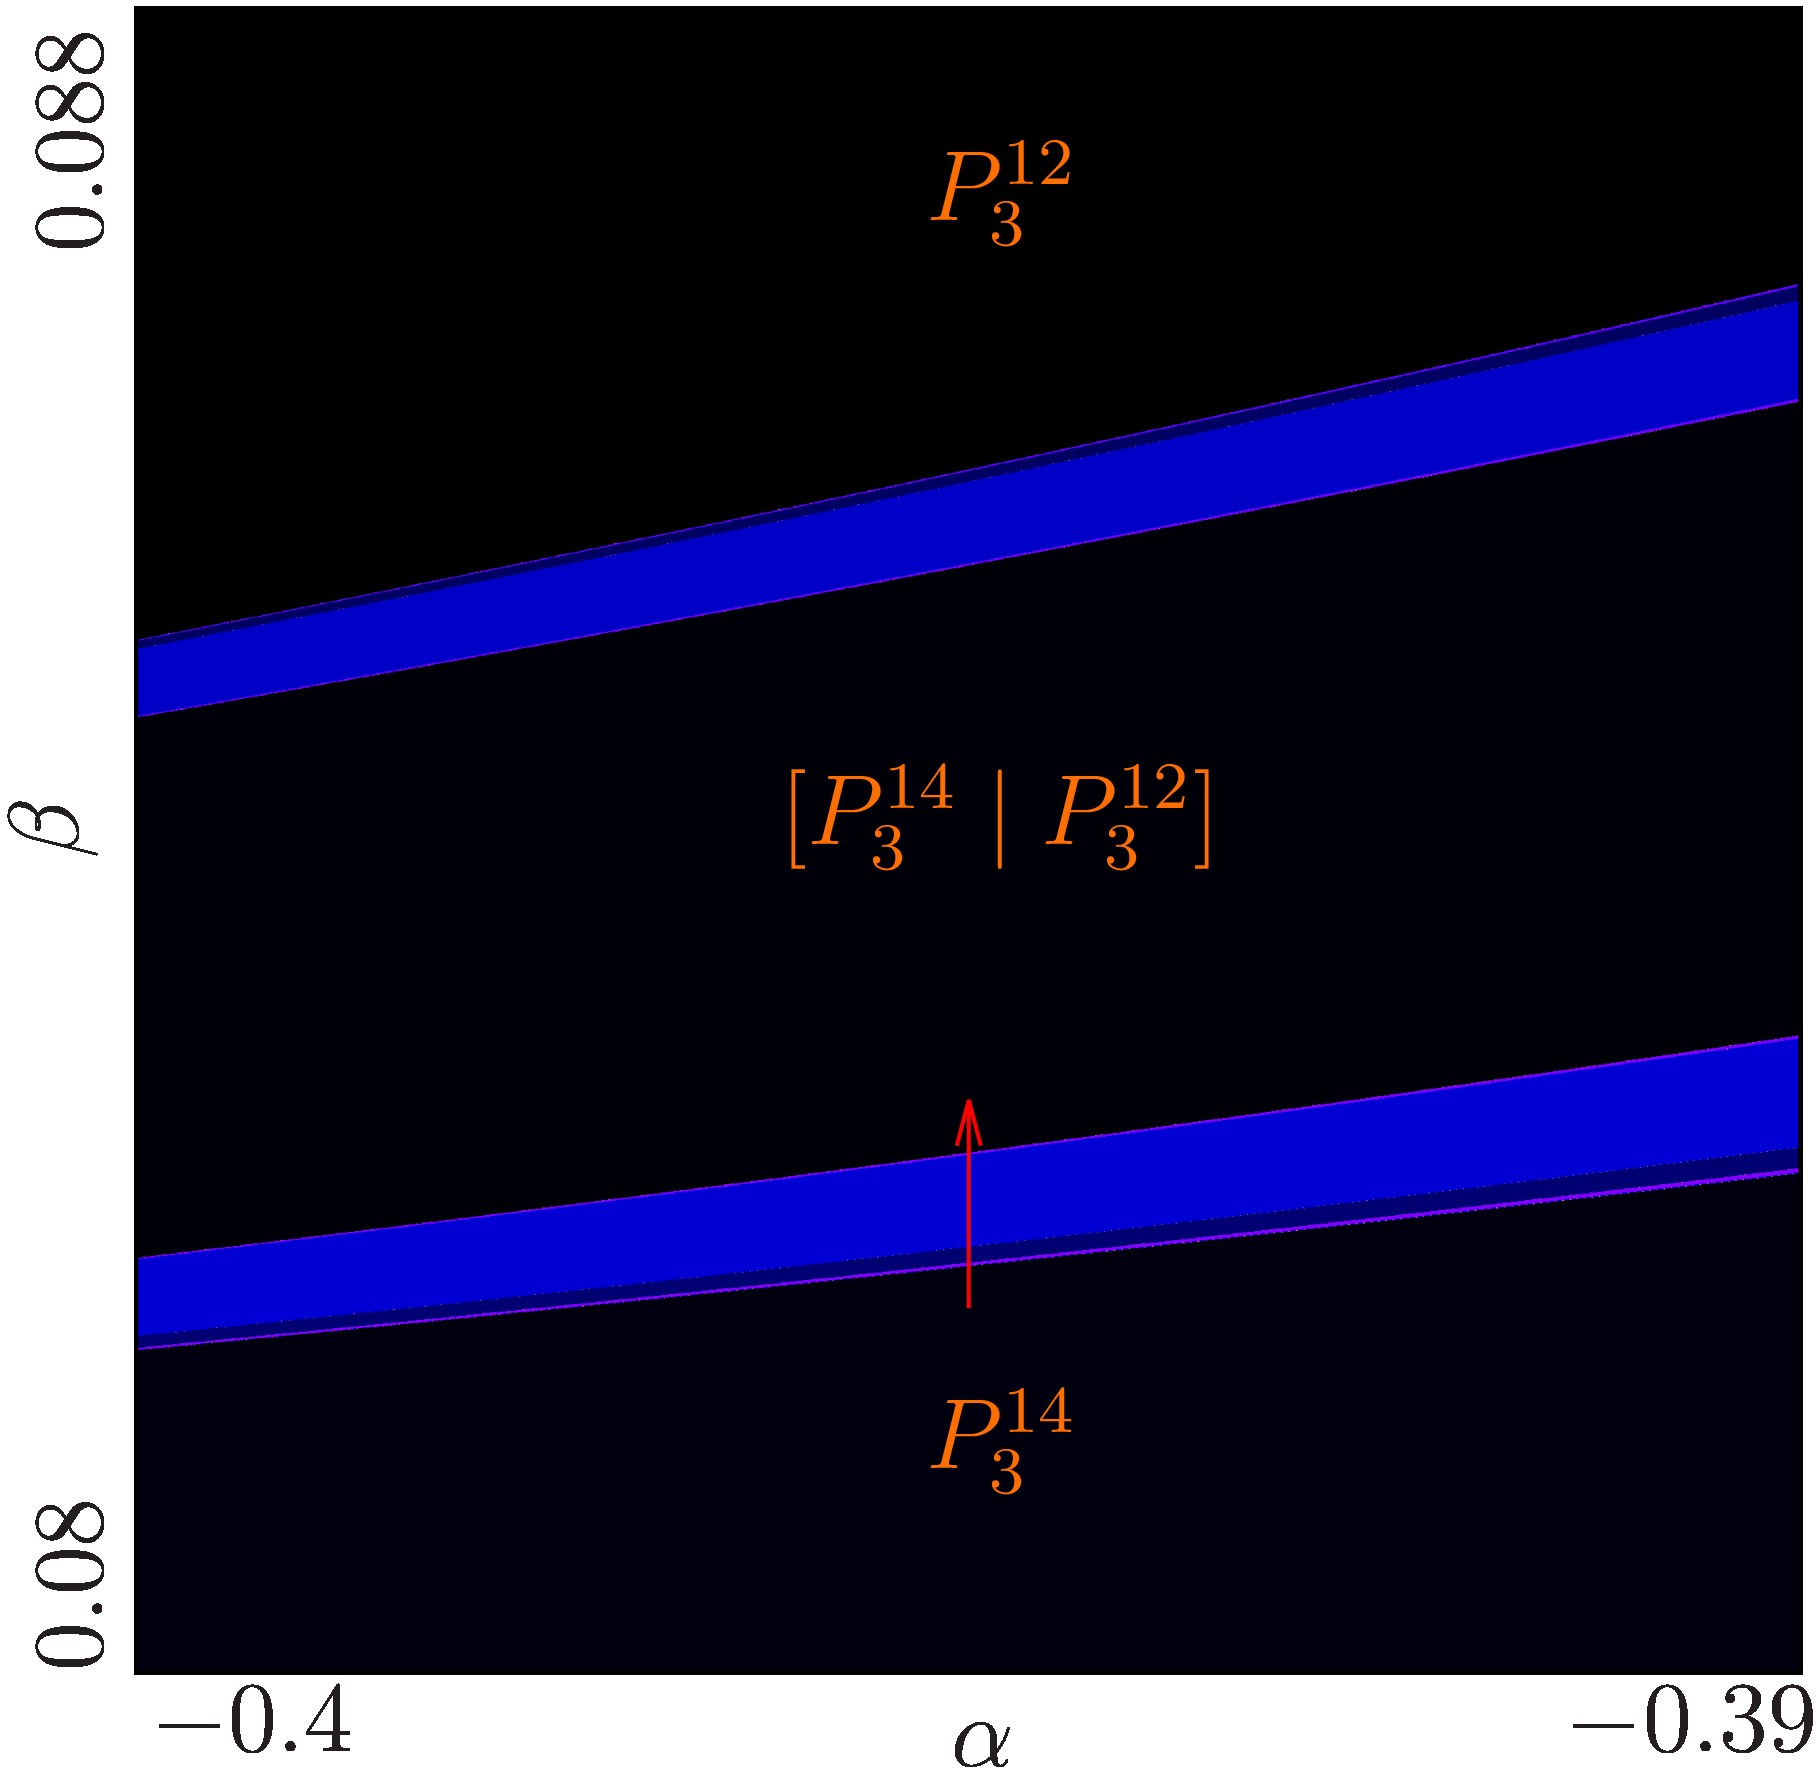
\includegraphics[width=.45 \textwidth]{../Figures/7/7.12a/result.png}
		\label{fig:add.add.like.hor.2D}
	}
	\subfloat[1D period scan]{
		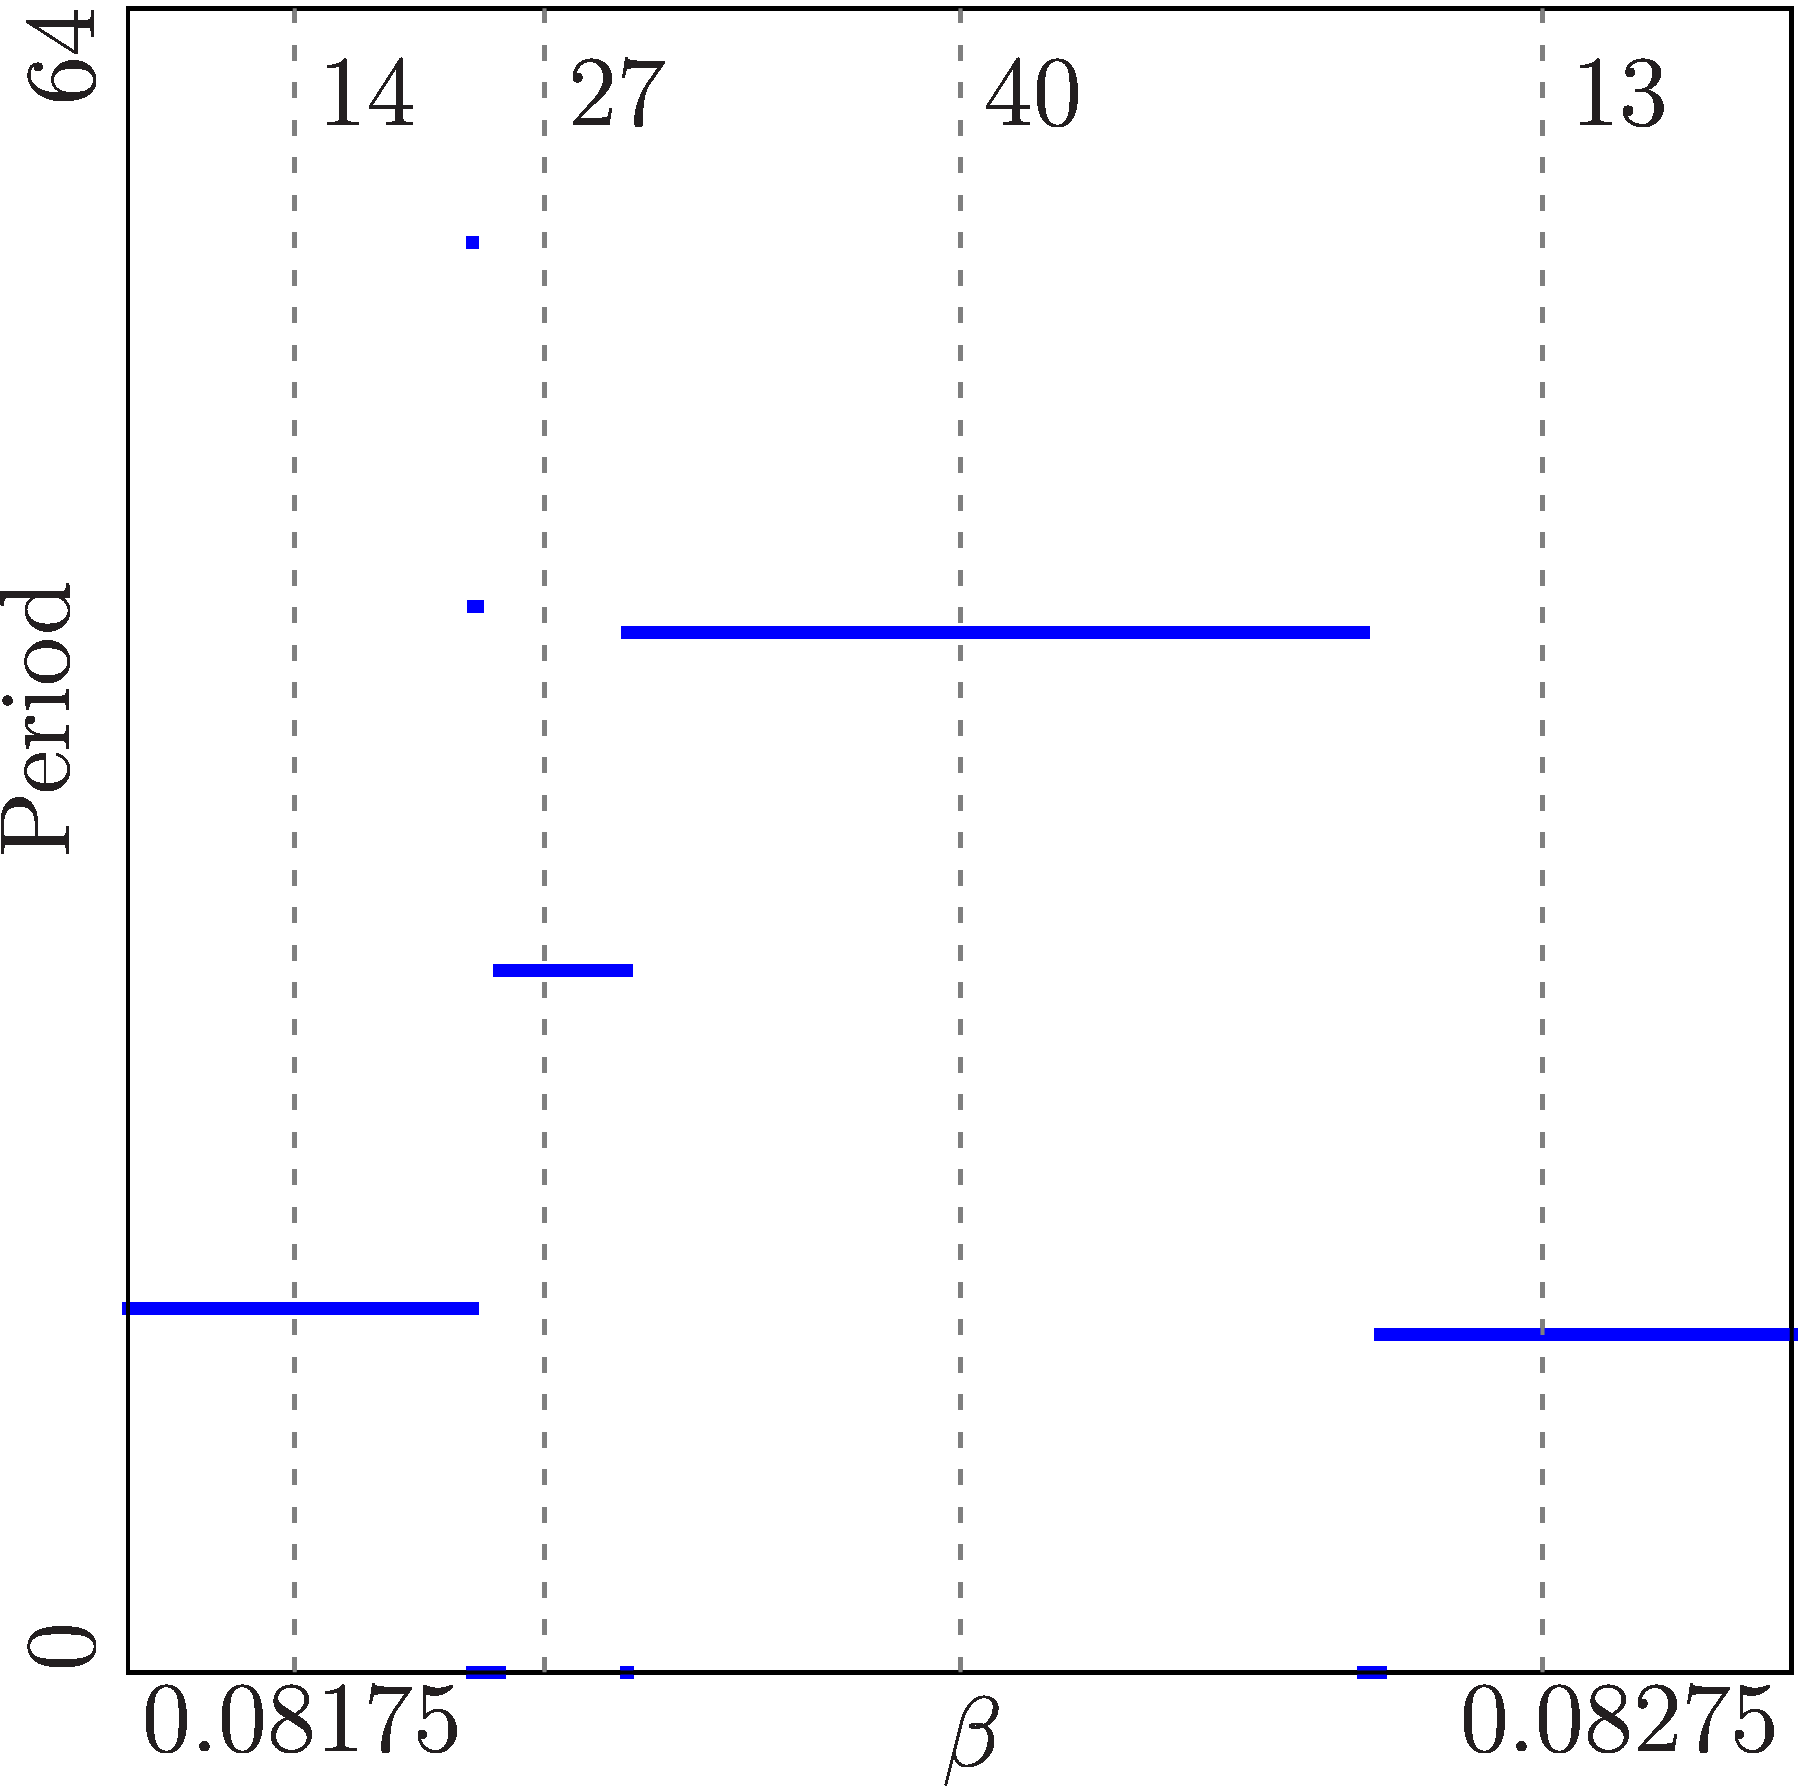
\includegraphics[width=.45 \textwidth]{../Figures/7/7.12b/result.png}
		\label{fig:add.add.like.hor.1D}
	}
	\caption[2D and 1D period scans of horizontal period-adding-like structures in the increasing archetypal model]{
		2D and 1D period scans of horizontal period-adding-like structures in the increasing archetypal model.
		The fixed parameters are $a_L = 1, b_L = 0.8,$ and $g_R\left(\frac{1}{2}\right) = \frac{1}{2} + \frac{1}{40}$.
		(a) shows the 2D period scan where the parameters $\alpha = g_R\left(\frac{1}{4}\right)$ and $\beta = c_L$ are varied.
		The small arrow indicates the parameter range for the 1D period scan in (b).
		Here, only $\beta$ is varied.
		The numbers at the top mark the periods at the corresponding value for $\beta$.
	}
	\label{fig:add.add.like.hor}
\end{figure}

The structure is not just a skewed \gls{pa} structure, as one might think since the period $27$ is associated with another parameter region that is not the most pronounced between the parameter regions associated with the periods $14$ and $13$, respectively.
And also $27 + 13 = 40$ which is associated with the parameter region between the parameter regions associated with the periods $27$ and $13$, respectively.
We can see that when examining the symbolic sequences associated with the parameter regions in that structure.
\Cref{fig:add.add.like.hor.tree} shows the Farey-tree with the symbolic sequences of this structure.
The starting nodes are associated with the symbolic sequences associated with the parameter regions $P^{14}_3$ and $\left[P^{14}_3 \mid P^{12}_3\right]$, respectively.
The parameter region associated with the period $27$ is the lowest node in level $2$, which is associated with two coexisting cycles.
These two cycles, $\A^4\B^3\C^4\D^3\A^4\B^3\C^3\D^3$ and $\A^4\B^3\C^4\D^3\A^3\B^3\C^4\D^3$ could be the result of concatenating the symbolic sequences $A^4\B^3\C^4\D^3$ and $\A^4\B^3\C^3\D^3$, as well as $\A^4\B^3\B^4\D^3$ and $\A^3\B^3\C^4\D^3$ of the parameter regions associated with the periods $14$ and $13$, respectively.
But the cycle $\A^4\B^3\C^4\D^3\A^3\B^3\B^4\D^3\A^4\B^3\C^3\D^3$ of the parameter region associated with the period $40$ cannot be a result of concatenating any pair of symbolic sequences $\A^4\B^3\C^3\D^3$ and $\A^3\B^3\C^4\D^3$ of the parameter region associated with the period $13$ and $\A^4\B^3\C^4\D^3\A^4\B^3\C^3\D^3$ and $\A^4\B^3\C^4\D^3\A^3\B^3\C^4\D^3$ of the parameter region associated with the period $27$.
One can see that this is truly no \gls{pa} structure.

\begin{figure}
	\centering
	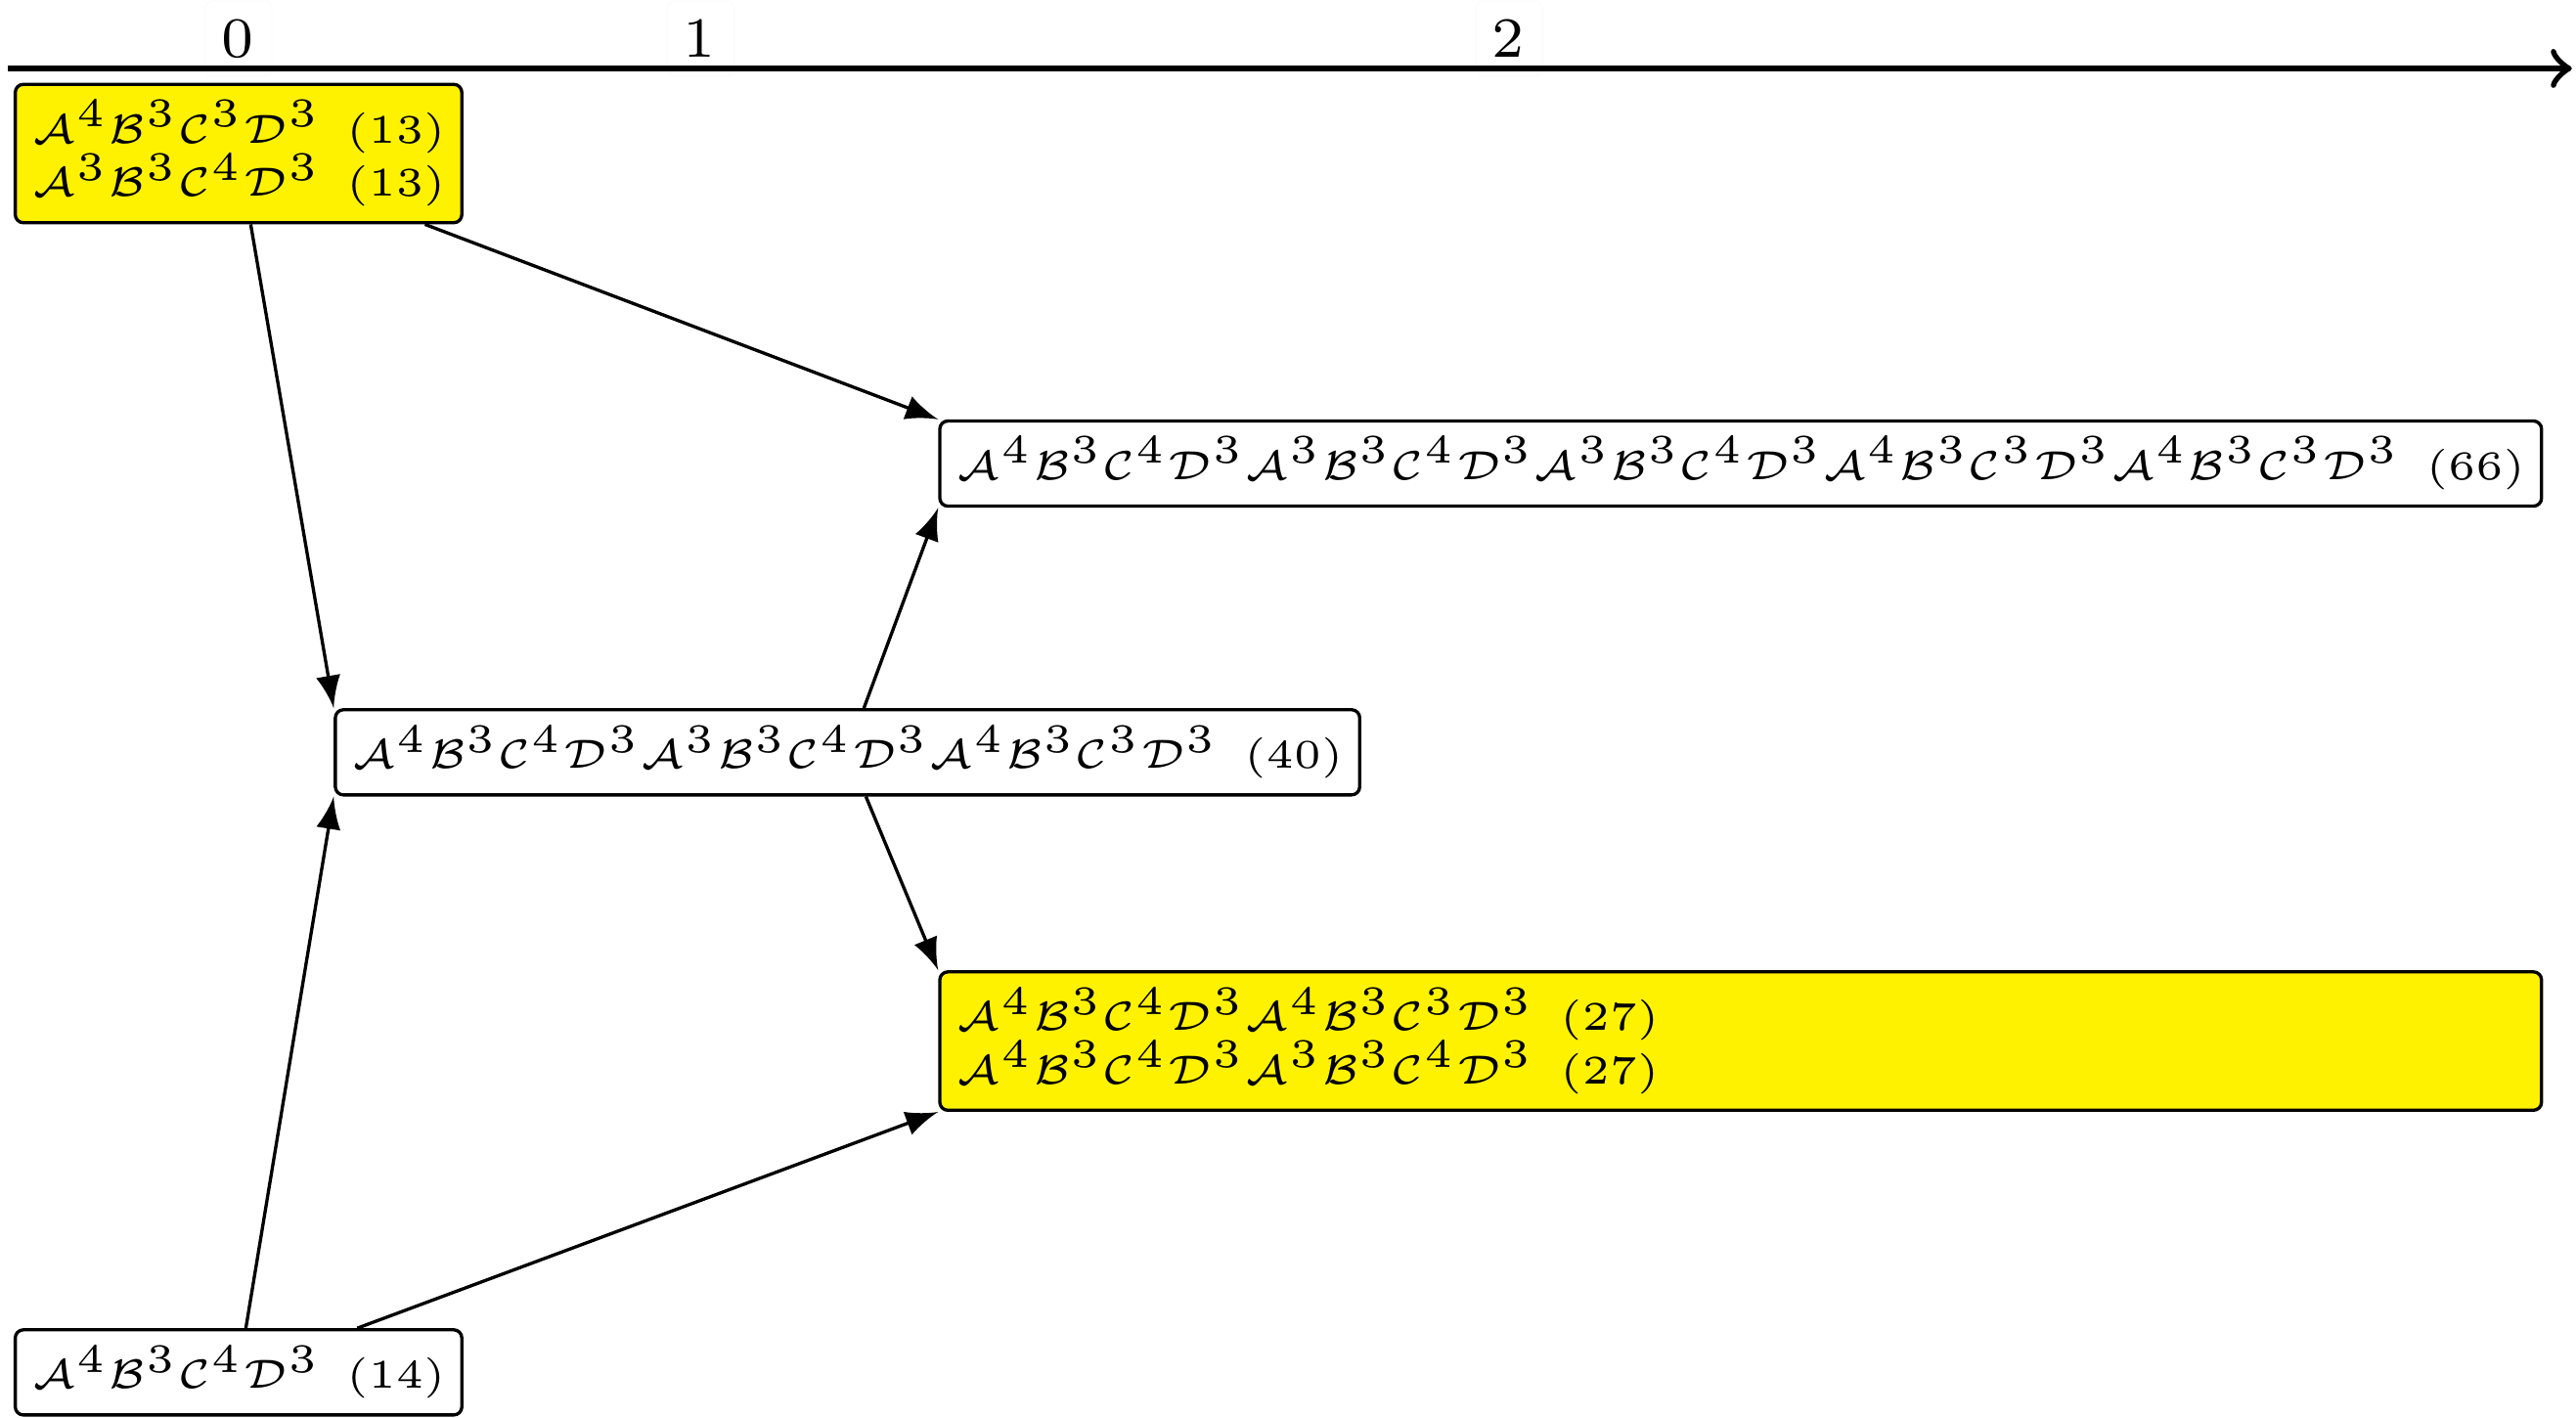
\includegraphics[width=.7 \textwidth]{../Figures/7/7.13/adding.png}
	\caption[Farey-tree with the symbolic sequences of a horizontal \glsentrylong{pal} structure]{
		Farey-tree with the symbolic sequences associated with the parameter regions of the lower horizontal \gls{pal} structure marked with a red arrow in \Cref{fig:add.add.like.hor.2D} up to two levels.
		Nodes of parameter regions associated with two coexisting cycles are colored yellow.
	}
	\label{fig:add.add.like.hor.tree}
\end{figure}

\subsubsection{Vertical Period-adding-like Structures}

Next, vertically oriented \gls{pal} structures \hl{are examined}.
\Cref{fig:add.add.like.vert.2D} shows a 2D period scan of this structure.
Here, we can also see two \gls{pal} structures, one in-between the parameter regions $P^{12}_2$ and $\left[P^{12}_2 \mid P^{14}_3\right]$ and one in-between the parameter regions $\left[P^{12}_2 \mid P^{14}_3\right]$ and $P^{14}_3$.
\hl{T}he \gls{pal} structure in-between the parameter regions $P^{12}_2$ and $\left[P^{12}_2 \mid P^{14}_3\right]$ \hl{is chosen} for closer investigation.
\hl{Again,} a red arrow marks the parameter range for the 1D period scan of this \gls{pal} structure in \Cref{fig:add.add.like.vert.1D}.

As before, the periods do not add as we would expect from a \gls{pa} structure.
The most pronounced parameter region between the parameter regions associated with the periods $12$ and $13$ is associated with the period $38$.
And the most pronounced parameter region between this parameter region and the parameter region associated with the period $12$ is associated with the period $25$, which should have been the most pronounced parameter region between the parameter regions associated with the periods $12$ and $13$, respectively.

\begin{figure}
	\centering
	\subfloat[2D period scan]{
		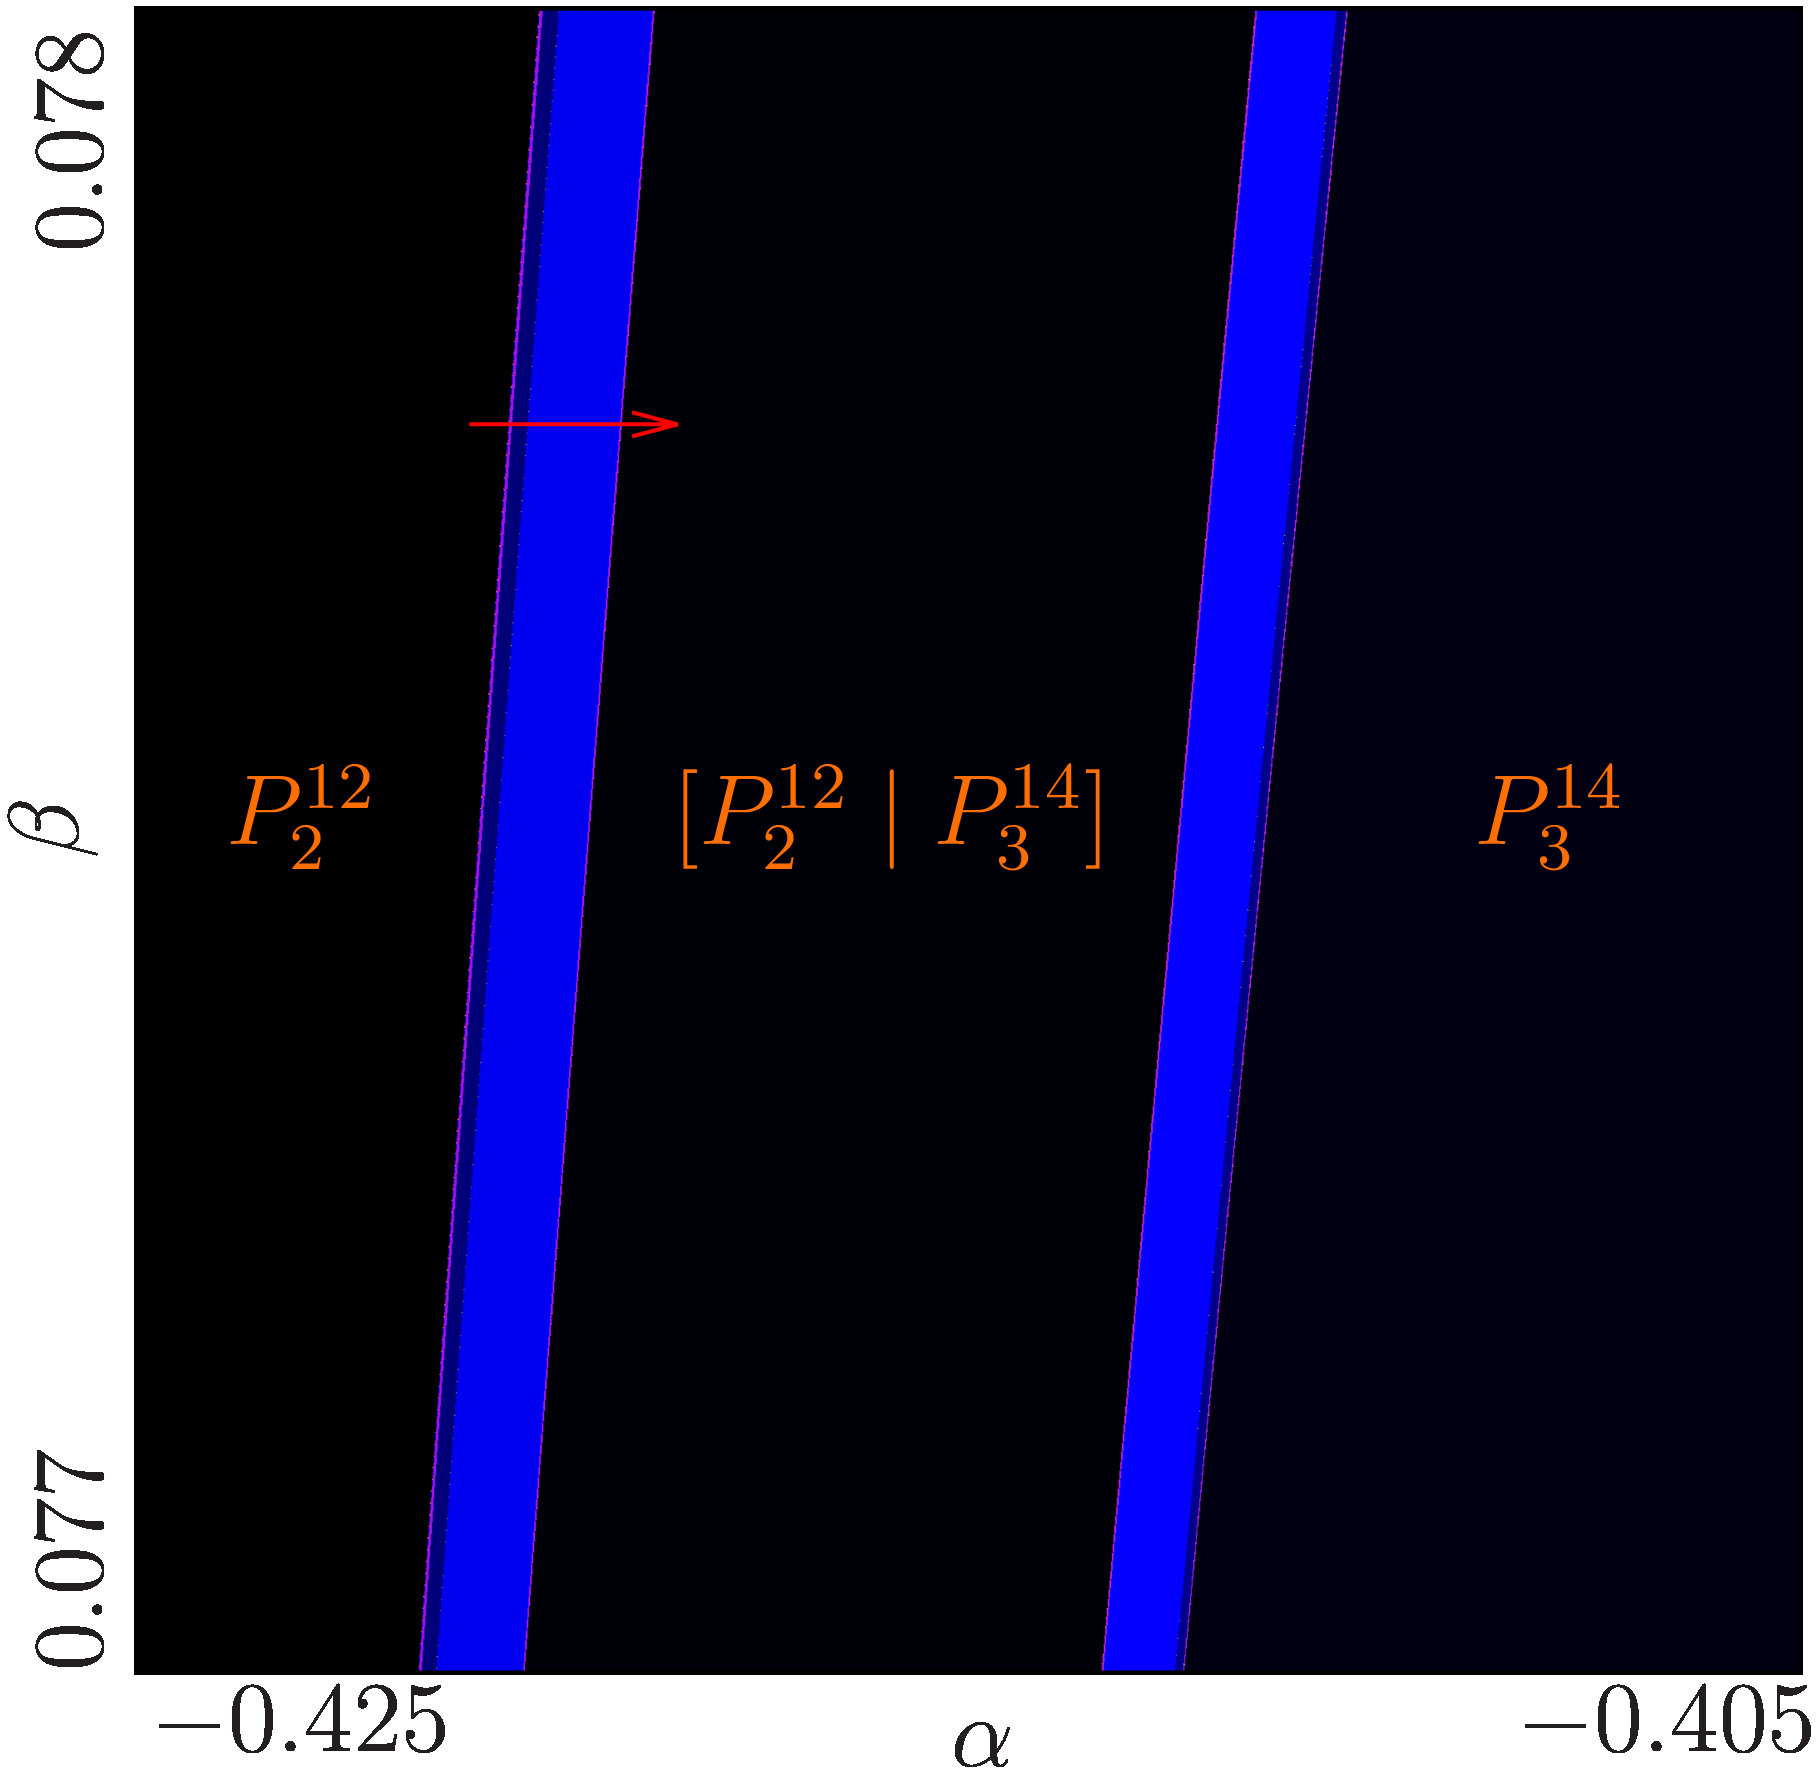
\includegraphics[width=.45 \textwidth]{../Figures/7/7.14a/result.png}
		\label{fig:add.add.like.vert.2D}
	}
	\subfloat[1D period scan]{
		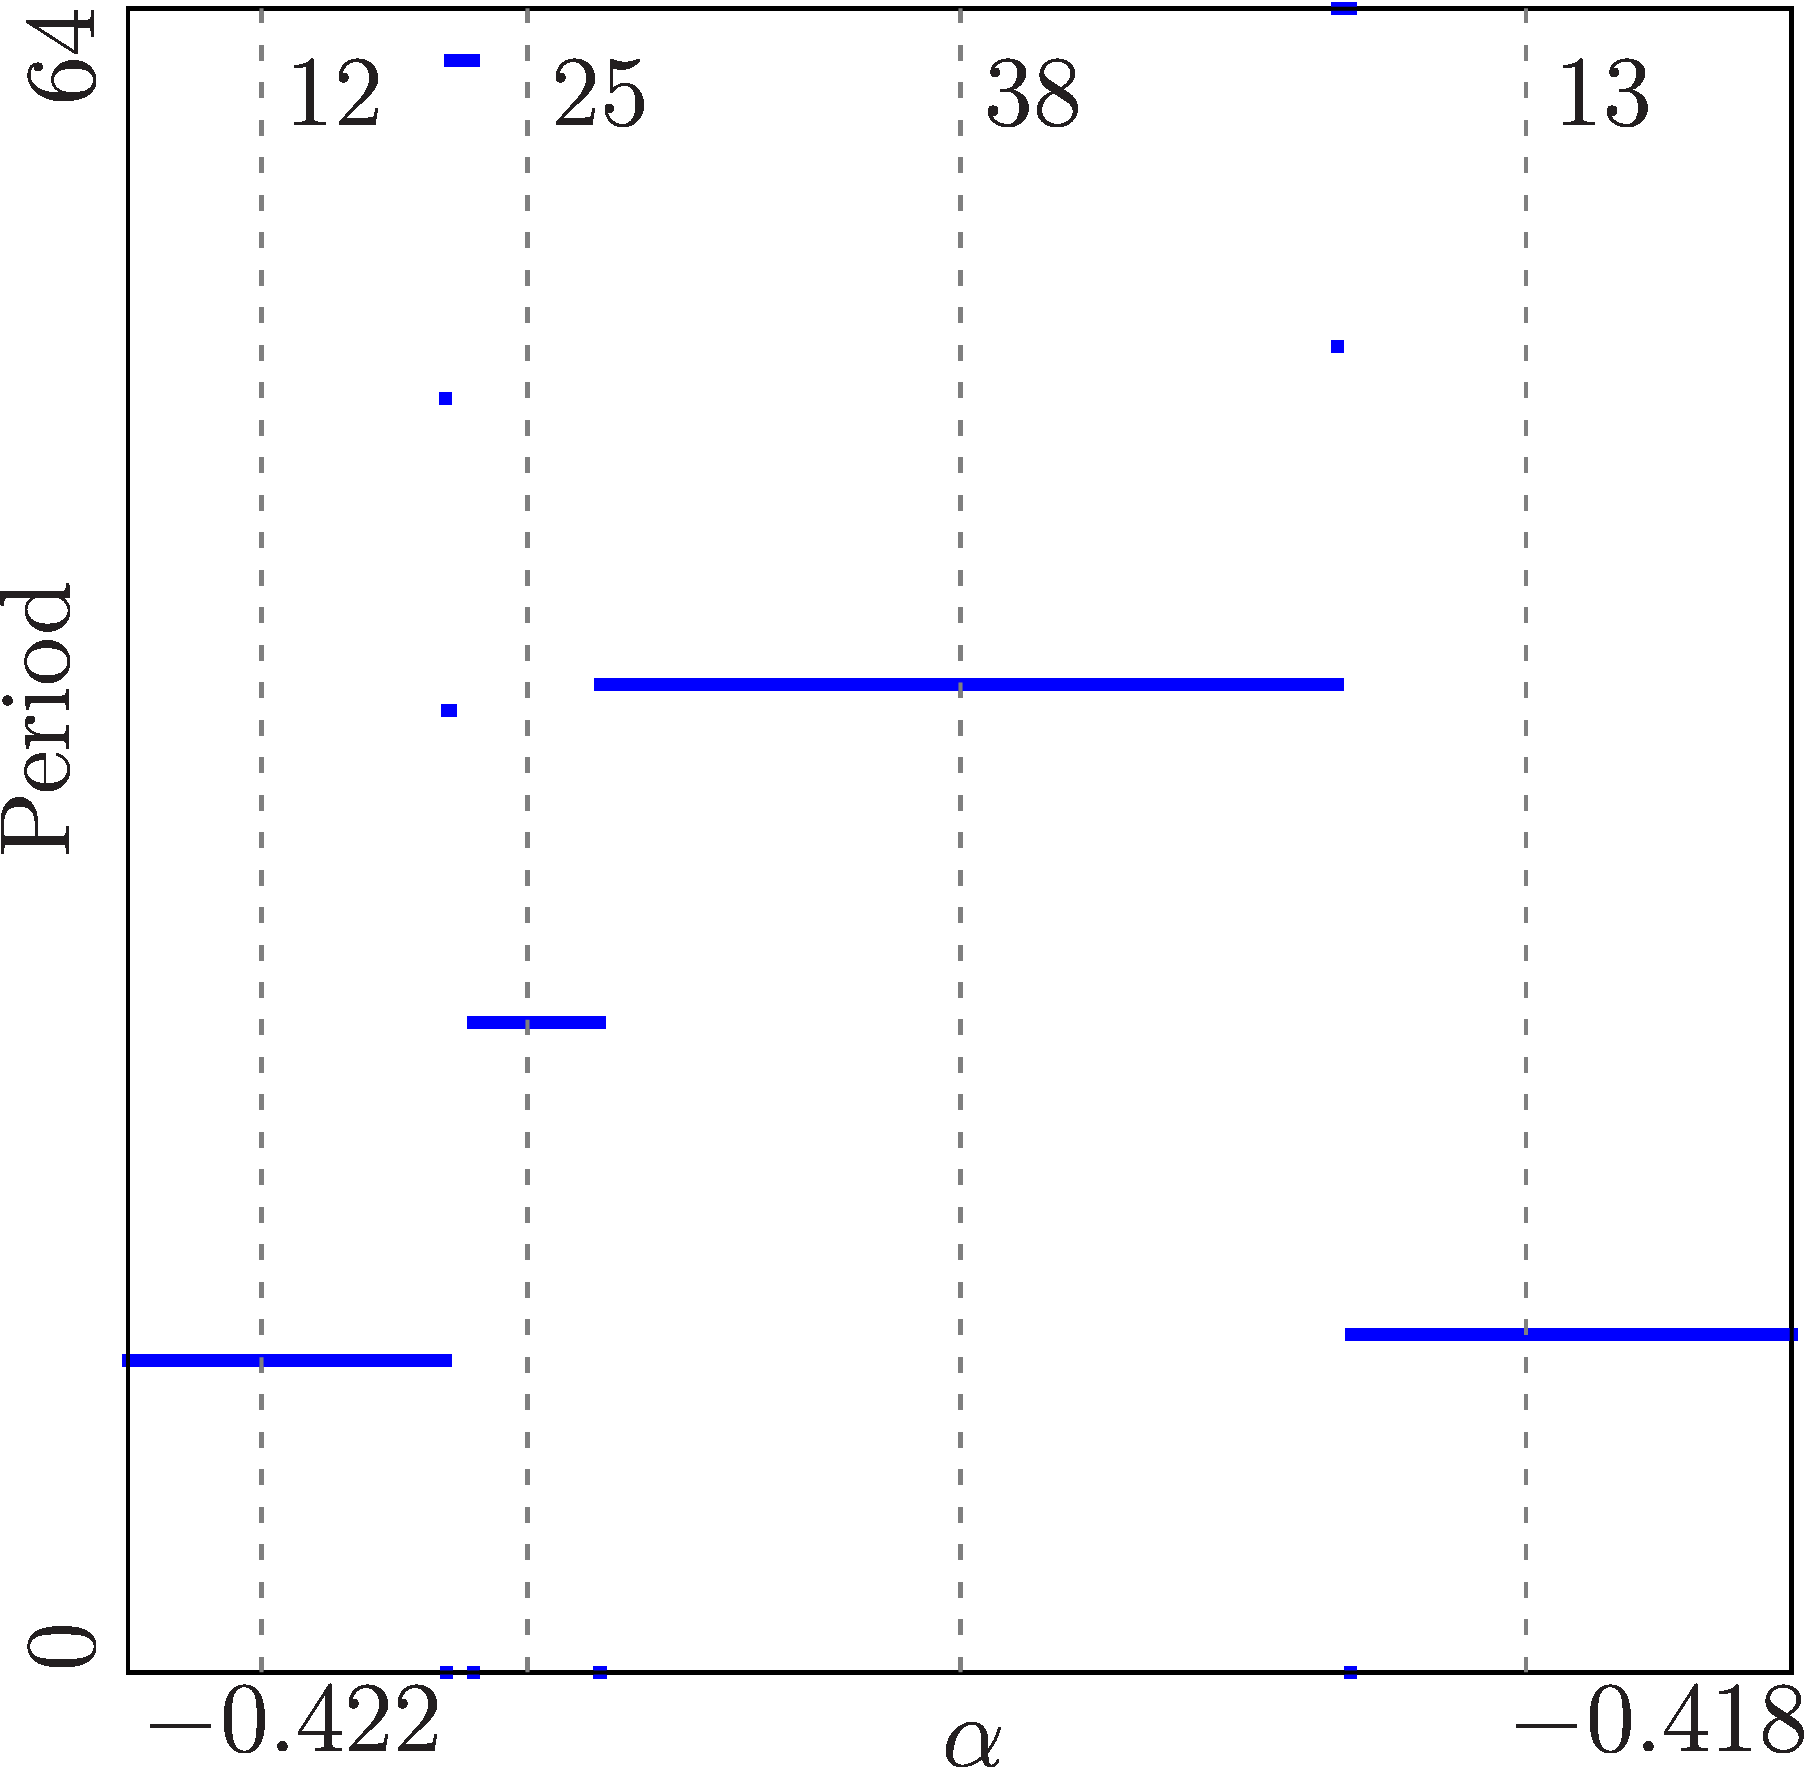
\includegraphics[width=.45 \textwidth]{../Figures/7/7.14b/result.png}
		\label{fig:add.add.like.vert.1D}
	}
	\caption[2D and 1D period scans of vertical period-adding-like structures in the increasing archetypal model]{
		2D and 1D period scans of vertical period-adding-like structures in the increasing archetypal model.
		The fixed parameters are $a_L = 1, b_L = 0.8,$ and $g_R\left(\frac{1}{2}\right) = \frac{1}{2} + \frac{1}{40}$.
		(a) shows the 2D period scan where the parameters $\alpha = g_R\left(\frac{1}{4}\right)$ and $\beta = c_L$ are varied.
		The small arrow indicates the parameter range for the 1D period scan in (b).
		Here, only $\alpha$ is varied.
		The numbers at the top mark the periods at the corresponding value for $\alpha$.
	}
	\label{fig:add.add.like.vert}
\end{figure}

Again, a Frey-tree with the symbolic sequences associated with the parameter regions in this \gls{pal} structure \hl{is provided} in \Cref{fig:add.add.like.vert.tree}.
One can see that the expected concatenation of the symbolic sequence does not work.
Nor does the concatenation of the symbolic sequence of the parameter region associated with the period $25$, which is the lowest node in level $2$, with the symbolic sequences of the parameter region associated with the period $13$, which is the upper starting node, to get the symbolic sequences of the period region of the parameter region associated with the period $38$, which is the only node in level $1$.
\hl{
	Therefore, this is no \gls{pa} structure either.
}

\begin{figure}
	\centering
	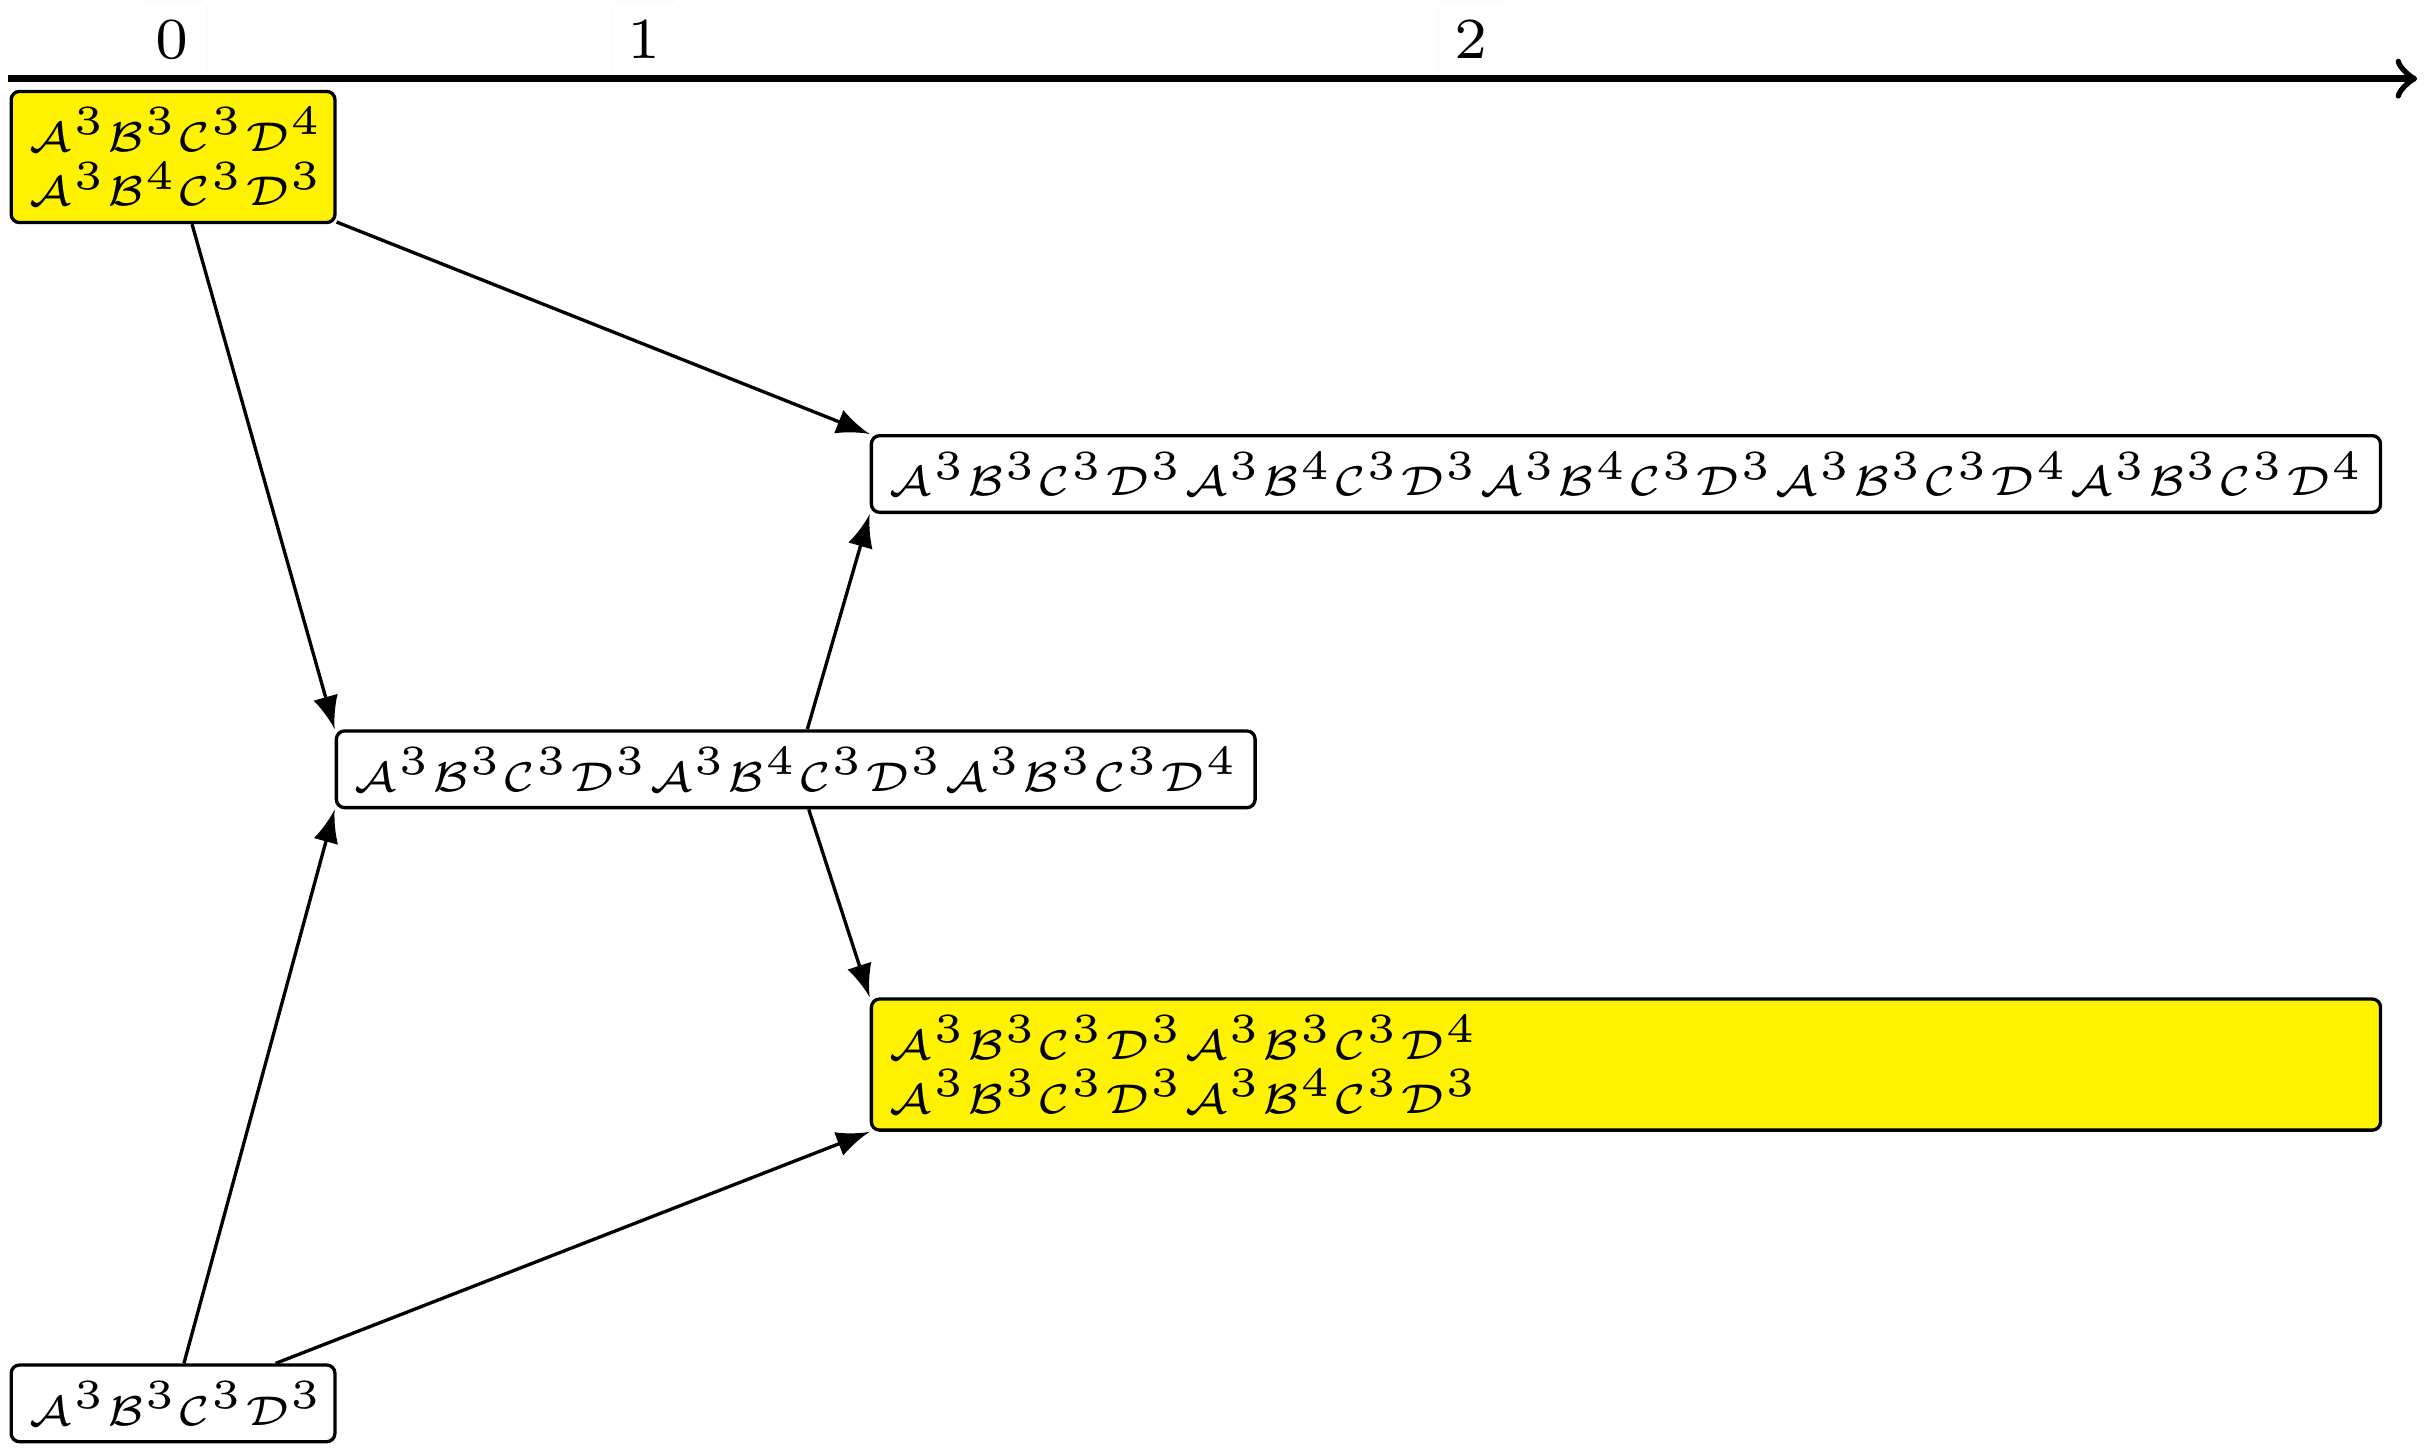
\includegraphics[width=.7 \textwidth]{../Figures/7/7.15+17/adding.png}
	\caption[Farey-tree with the symbolic sequences of a horizontal \glsentrylong{pal} structure]{
		Farey-tree with the symbolic sequences associated with the parameter regions of the left vertical \gls{pal} structure marked with a red arrow in \Cref{fig:add.add.like.vert.2D} up to two levels.
		Nodes of parameter regions associated with two coexisting cycles are colored yellow.
	}
	\label{fig:add.add.like.vert.tree}
\end{figure}

\subsubsection{Period-adding-like Structures in the Corners}

Finally, the structure in the corner which \Cref{fig:add.add.like.corn.2D} shows a 2D period scan of \hl{is examined}.
Here, we see many \gls{pal} structures.
These are organized as follows.
There is one horizontally oriented \gls{pal} structure between the parameter regions $\left[P^{12}_2 \mid P^{14}_3\right]$ and $P^{12}_3$.
And one horizontally oriented \gls{pal} structure between the parameter region $P^{12}_3$ and every parameter region in the vertically oriented \gls{pal} structure between the parameter regions $P^{12}_2$ and $\left[P^{12}_2 \mid P^{14}_3\right]$.
Analogously, there is one vertically oriented \gls{pal} structure between the parameter regions $P^{12}_2$ and $\left[P^{14}_3 \mid P^{12}_3\right]$.
And one vertically oriented \gls{pal} structure between the parameter region $P^{12}_2$ and every parameter region in the horizontally oriented \gls{pal} structure between the parameter regions $P^{14}_3$ and $\left[P^{14}_3 \mid P^{12}_3\right]$.
Similarly, there is also one horizontally oriented \gls{pal} structure between the parameter region $\left[P^{14}_3 \mid P^{12}_3\right]$ and every parameter region in the vertically oriented \gls{pal} structure between the parameter regions $\left[P^{12}_2 \mid P^{14}_3\right]$ and $P^{14}_3$.
And one vertically oriented \gls{pal} structure between the parameter region $\left[P^{12}_2 \mid P^{14}_3\right]$ and every parameter region in the horizontally oriented \gls{pal} structure between the parameter regions $P^{14}_3$ and $\left[P^{14}_3 \mid P^{12}_3\right]$.
A very similar phenomenon was discovered by \Citeauthor{tramontana2012period} where there are many \gls{pa} structures between some parameter region and every parameter region of a \gls{pa} structure~\cite{tramontana2012period}.

The 1D period scan in \Cref{fig:add.add.like.corn.1D} shows a 1D period scan of one of the simpler \gls{pal} structures.
It is the \gls{pal} structure between the parameter regions $P^{12}_2$ and $\left[P^{14}_3 \mid P^{12}_3\right]$ marked with a red arrow in \Cref{fig:add.add.like.corn.2D}.
The diagram looks exactly like the 1D period scan for the vertical \gls{pal} structure in \Cref{fig:add.add.like.vert.1D}.
Here, the periods also do not add up as we expect them to in \gls{pa} structures.

\begin{figure}
	\centering
	\subfloat[2D period scan]{
		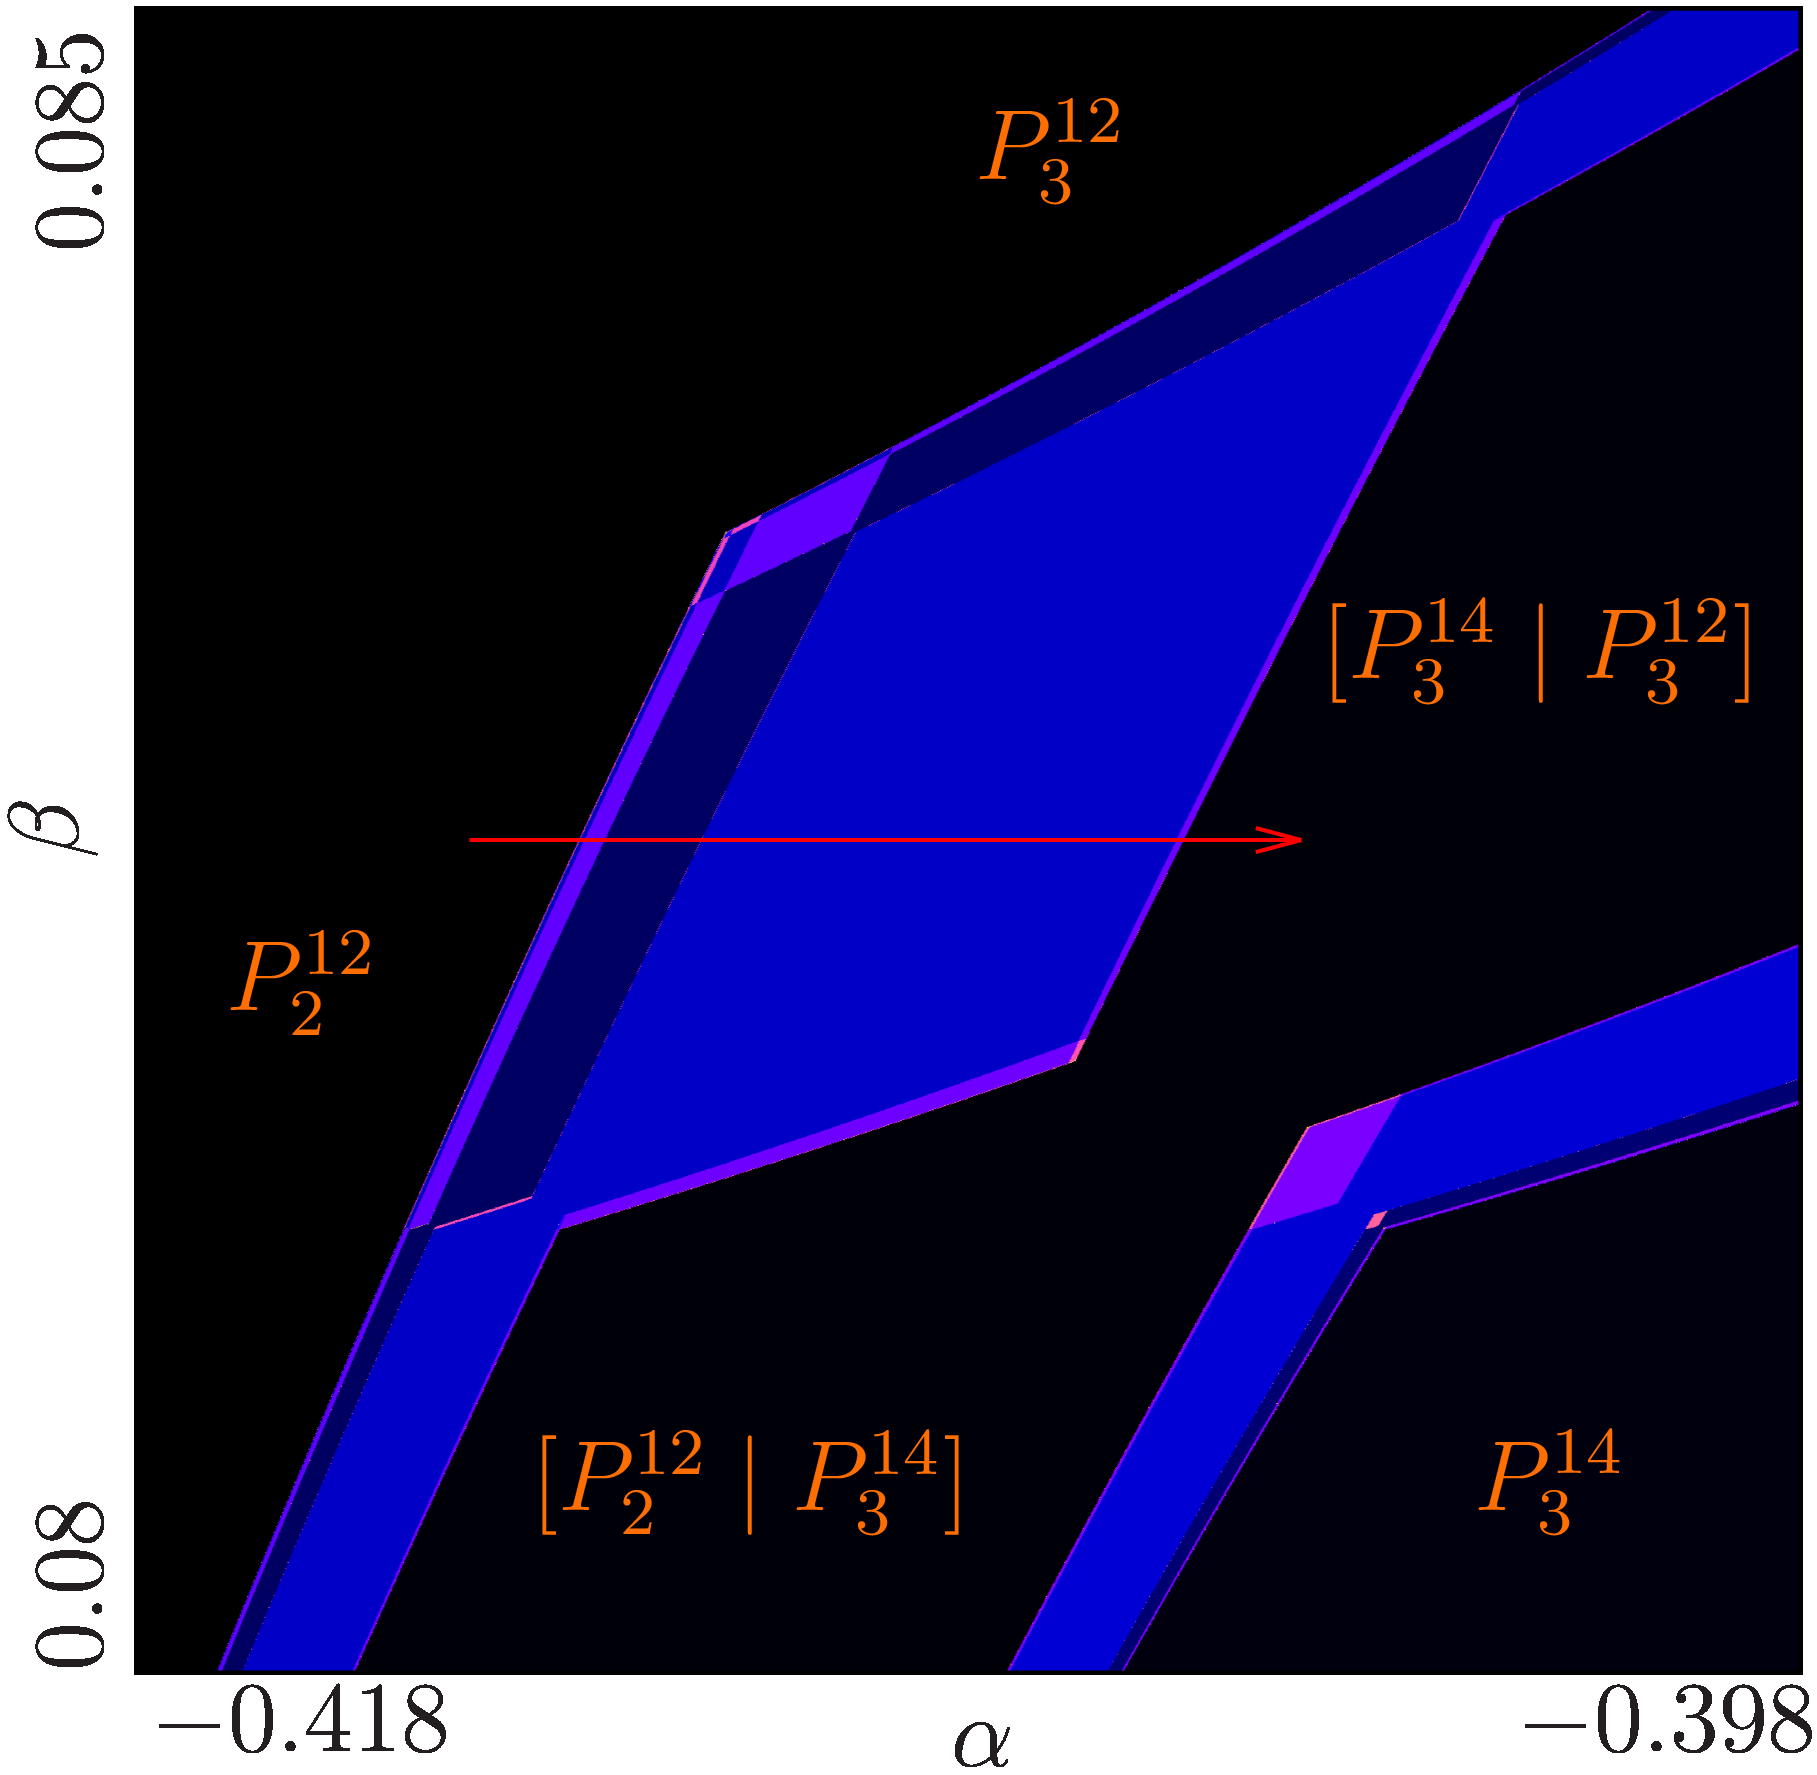
\includegraphics[width=.45 \textwidth]{../Figures/7/7.16a/result.png}
		\label{fig:add.add.like.corn.2D}
	}
	\subfloat[1D period scan]{
		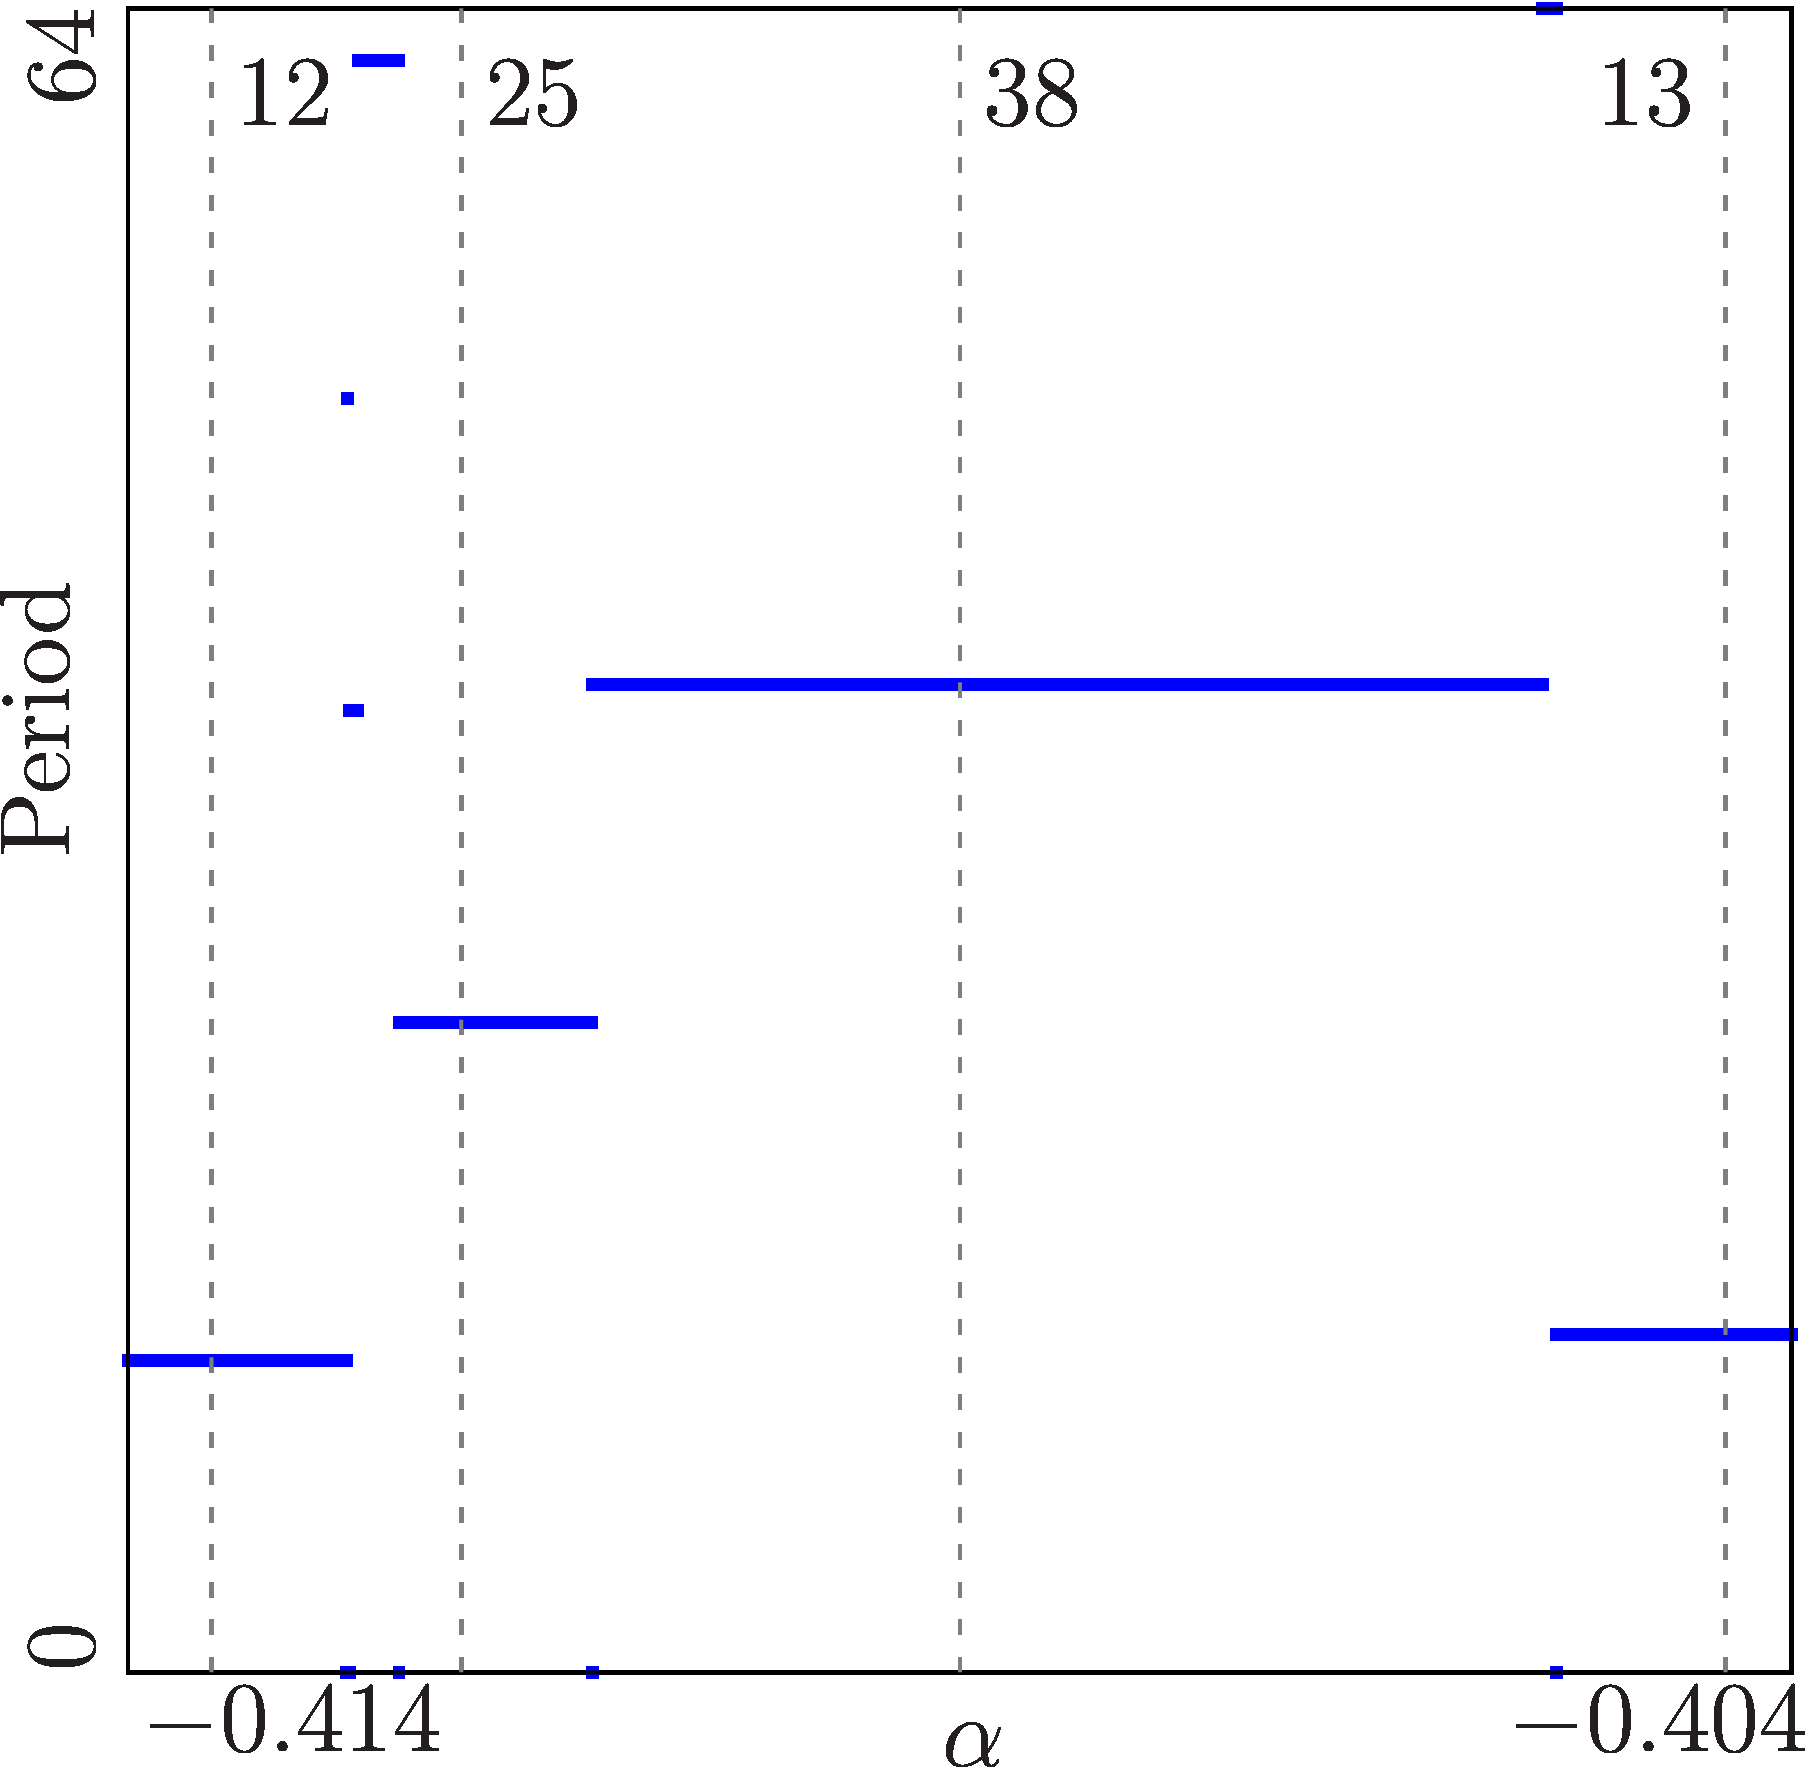
\includegraphics[width=.45 \textwidth]{../Figures/7/7.16b/result.png}
		\label{fig:add.add.like.corn.1D}
	}
	\caption[2D and 1D period scans of period-adding-like structures in the corners of the spaces between chains in the increasing archetypal model]{
		2D and 1D period scans of the period-adding-like structures in the corners of the spaces between chains in the increasing archetypal model.
		The fixed parameters are $a_L = 1, b_L = 0.8,$ and $g_R\left(\frac{1}{2}\right) = \frac{1}{2} + \frac{1}{40}$.
		(a) shows the 2D period scan where the parameters $\alpha = g_R\left(\frac{1}{4}\right)$ and $\beta = c_L$ are varied.
		The big arrow indicates the parameter range for the 1D period scan in (b).
		Here, only $\alpha$ is varied.
		The numbers at the top mark the periods at the corresponding value for $\alpha$.
	}
	\label{fig:add.add.like.corn}
\end{figure}

The symbolic sequences are different from the vertical \gls{pal} structure in \Cref{fig:add.add.like.vert.2D}.
Still the same argument as before works that this structure is not a skewed \gls{pa} structure.
Since there are infinitely many \gls{pal} structures in this corner it is very hard to describe each one and construct rules for the periods and symbolic sequences in the structures.
Luckily there is an easier way to describe the \gls{pal} structures in the increasing archetypal model and construct the wanted rules.
\hl{
	This involves the halved archetypal model, which is introduced in the next section.
}

\begin{figure}
	\centering
	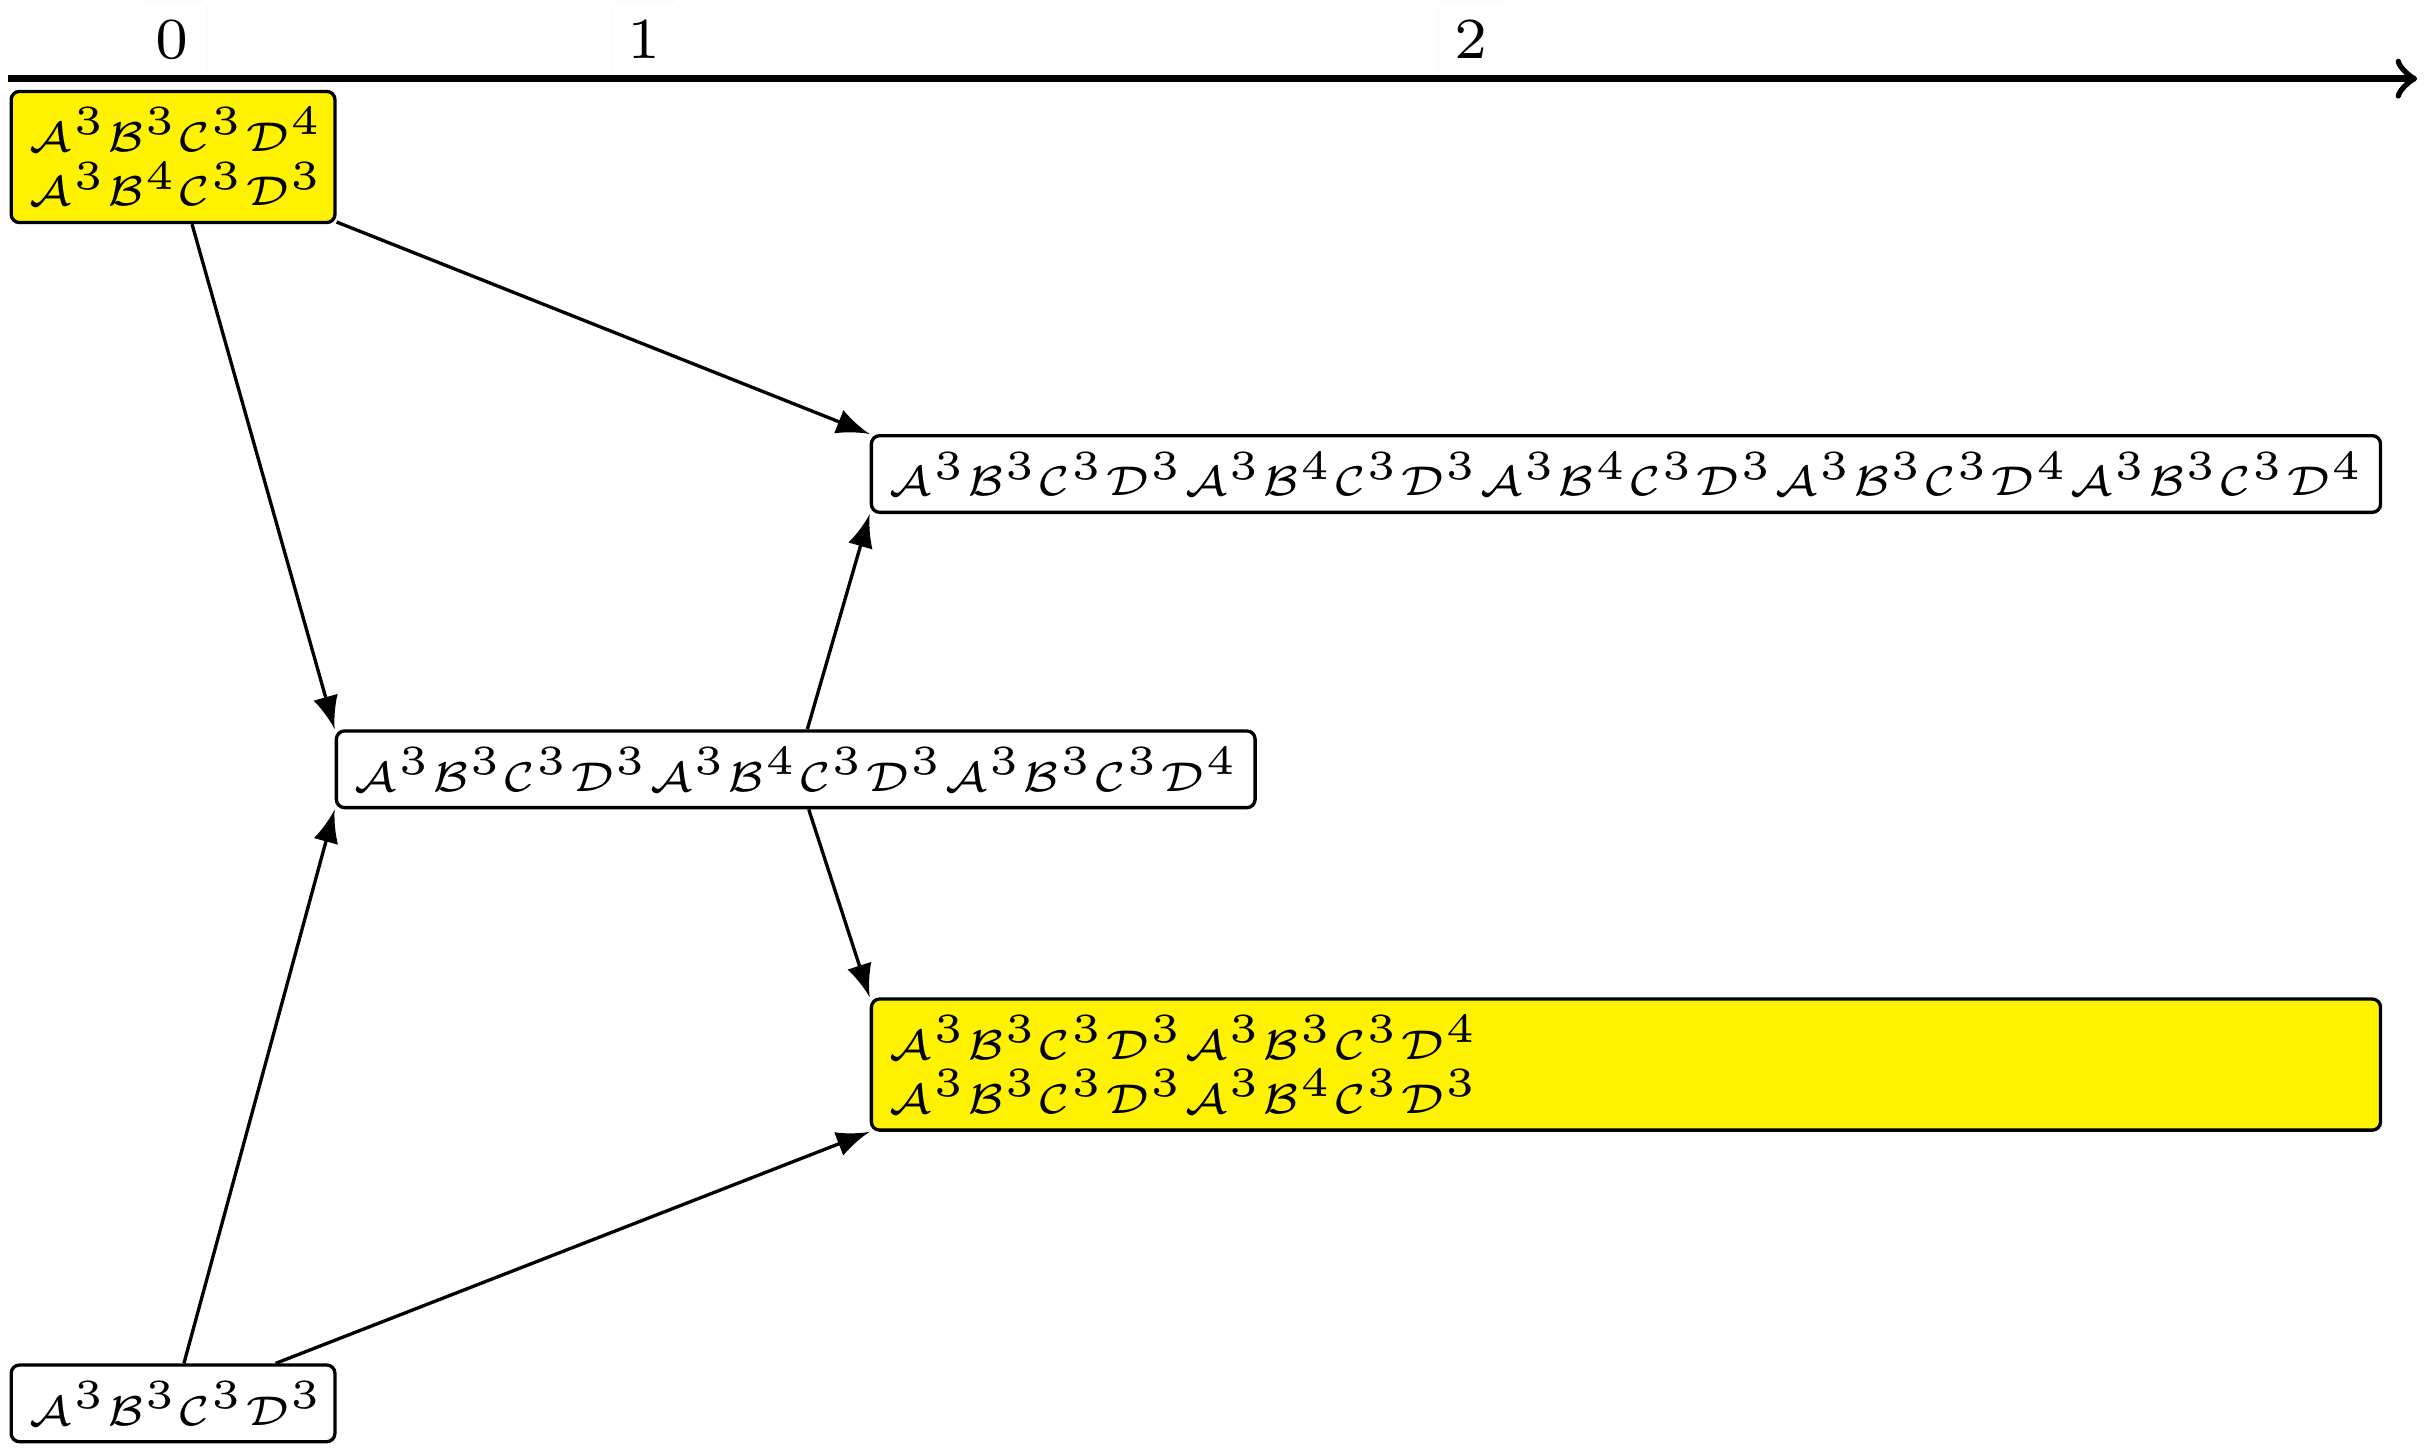
\includegraphics[width=.7 \textwidth]{../Figures/7/7.15+17/adding.png}
	\caption[Farey-tree with the symbolic sequences of a vertical \glsentrylong{pal} structure]{
		Farey-tree with the symbolic sequences associated with the parameter regions of the vertical \gls{pal} structure marked with a red arrow in \Cref{fig:add.add.like.corn.2D} up to two levels.
		Nodes of parameter regions associated with two coexisting cycles are colored yellow.
	}
	\label{fig:add.add.like.corn.vert.tree}
\end{figure}

\subsection{Halved Archetypal Model}
\label{sec:add.add.halved}

This section introduces the halved archetypal model.
First, the motivation and a definition is given.
After that, this section explains how this halved archetypal model is used to describe the \gls{pal} structures in the archetypal model.

\subsubsection{Motivation and Definition}

Since the archetypal model is a circle map, it can also be looked at as an infinite map.
Let $m$ be the archetypal model.
We know the model $m$ maps an input $x$ to $f(x) \mod 1$, meaning that if the output $f(x)$ is greater or equal to 1 we subtract 1 from it until it is in the range $[0, 1)$.
Similarly, we add 1 to it if it is smaller than 0 until it is in the desired range.
Now instead of confining the model to the domain of $[0, 1)$, we think of it repeating infinitely in both directions.
This process is called lifting of circle maps and is described by \Citeauthor{devaney2021introduction} in his book~\cite{devaney2021introduction}.
We can achieve this by mapping $T^m: x \mapsto f(x - \lfloor x \rfloor)$.
This trick maps any input $x \in \mathbb{R}$ into the domain $[0, 1)$ of the archetypal model $m$ and causes $T^m$ to repeat infinitely.
$T^m$ is now a lift of the model $m$ in the domain of all real numbers $\mathbb{R}$.
\Cref{fig:add.halved.lift} illustrates this concept for the cycle in the parameter region $P^{14}_3$.
The archetypal model in the lifted archetypal model is marked with a blue square.
These blue squares repeat infinitely in each direction.
One can see that the branch $f_\D$ is outside the blue square at its right edge.
This is because it was cut off and continued at the bottom of the square in the archetypal model, due to the $\mod 1$ operation.

\begin{figure}
	\centering
	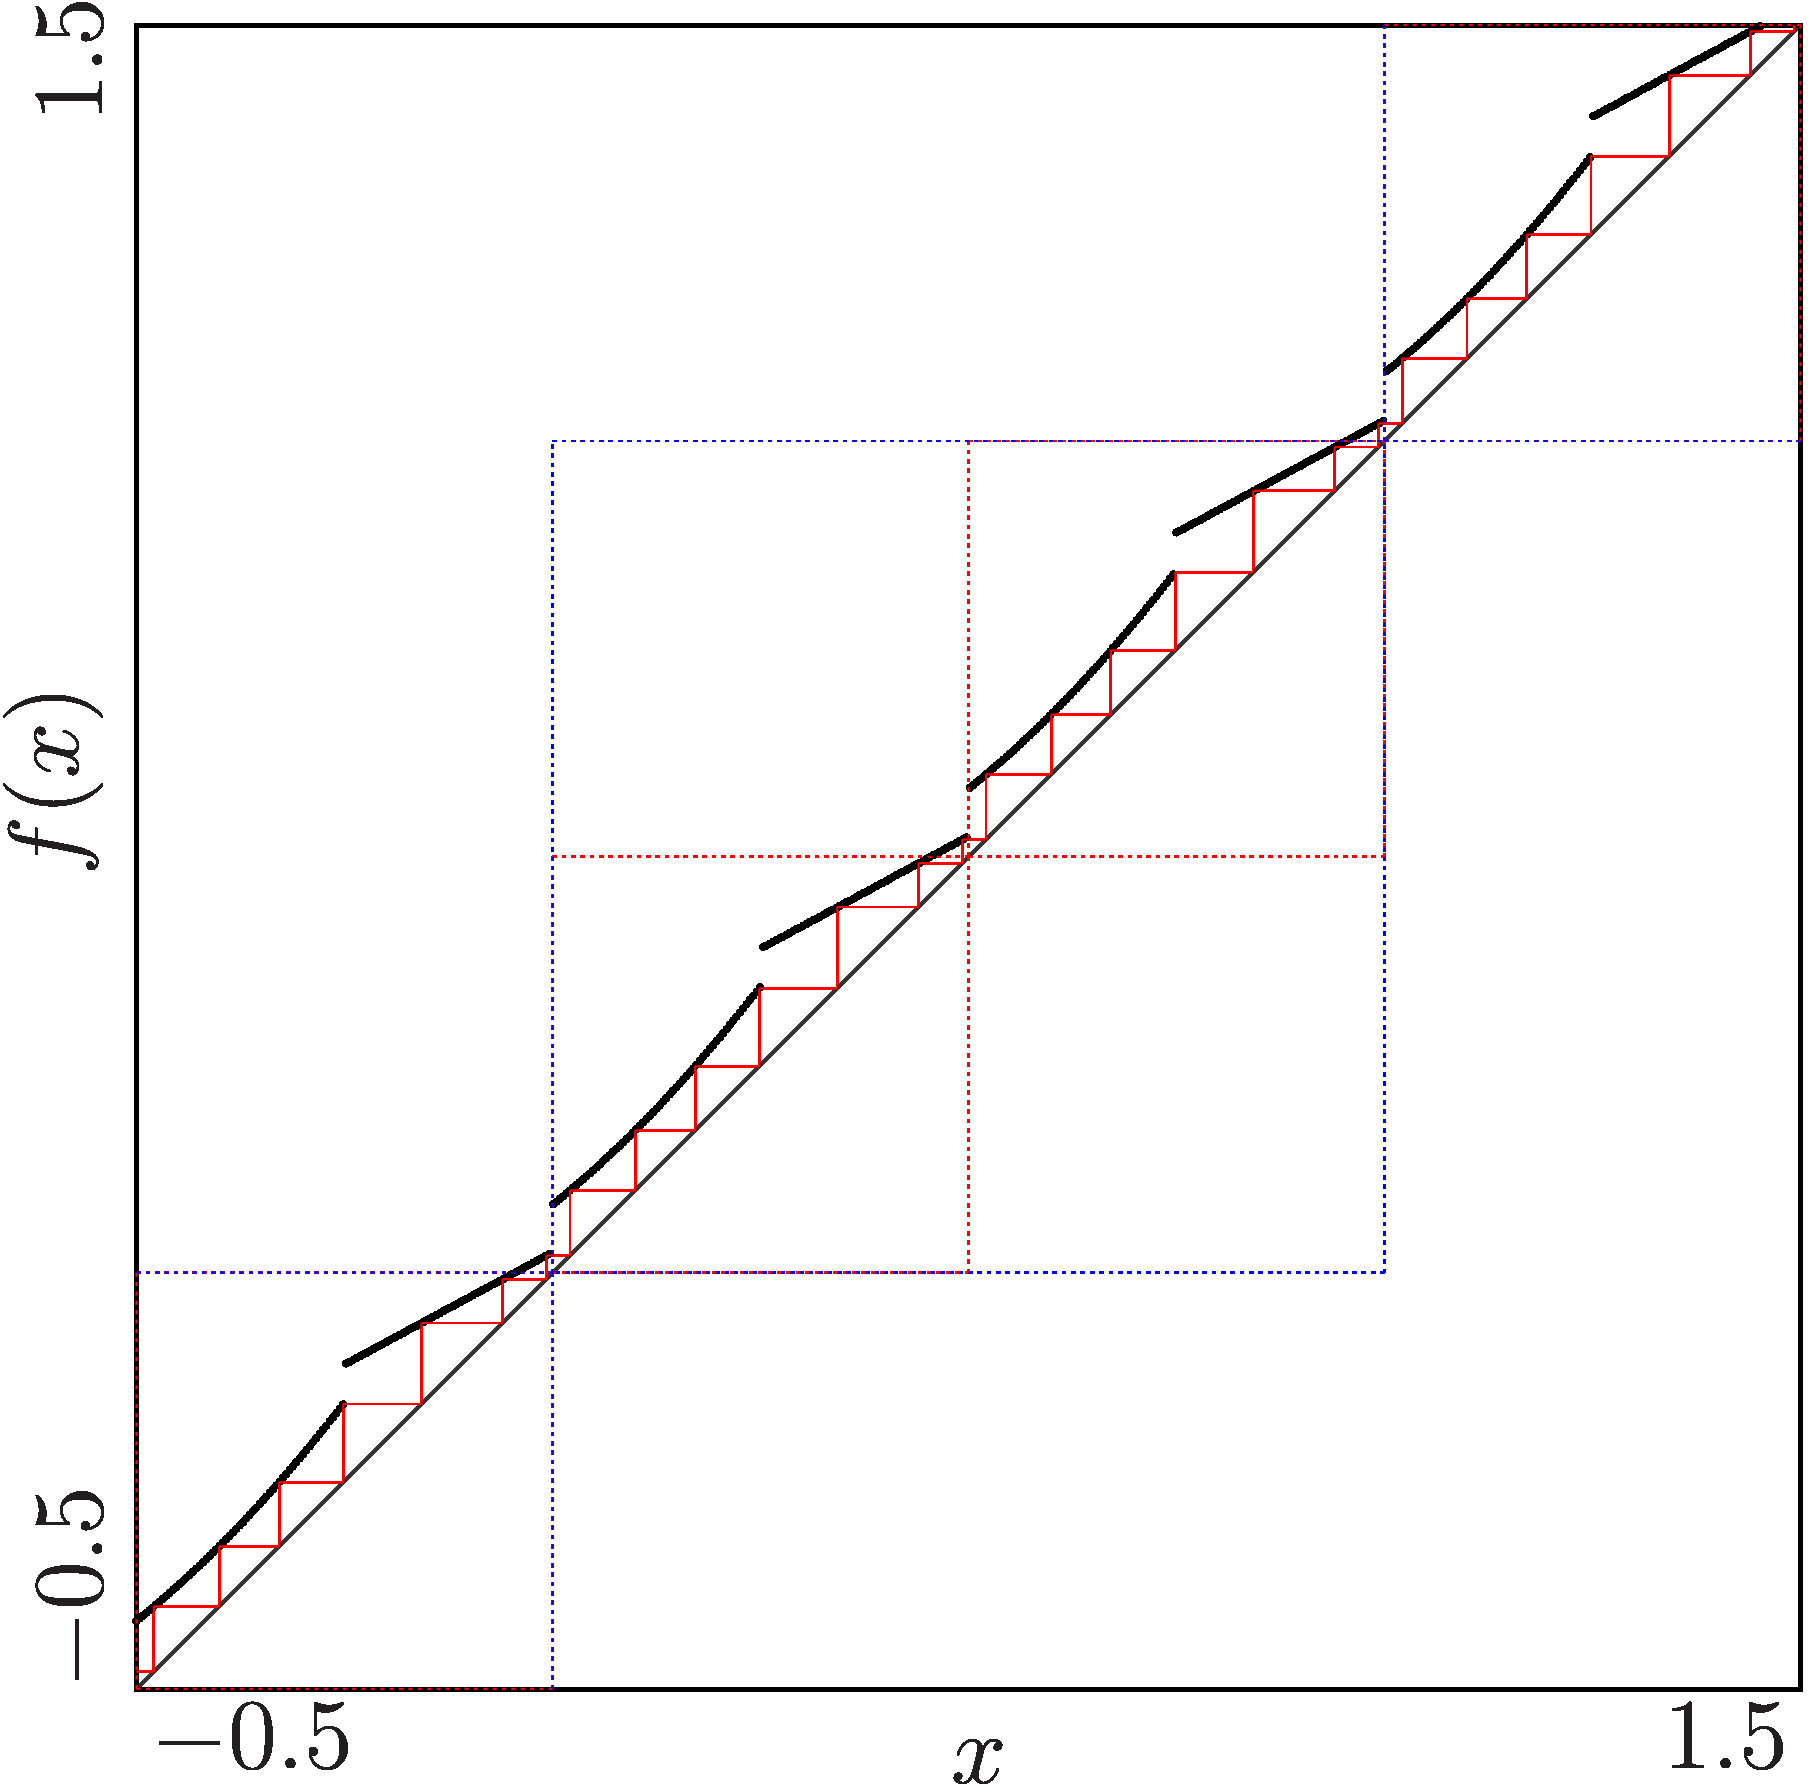
\includegraphics[width=.7 \textwidth]{../Figures/7/7.18/result.png}
	\caption[Illustration of the lifted archetypal model]{
		Illustration of the lifted archetypal model.
	}
	\label{fig:add.halved.lift}
\end{figure}

In this model, there are no cycles that have multiple rotations.
Instead, the cycles that had multiple rotations in the archetypal model, manifest as a sequence of different blocks of the archetypal model.
Meaning, for the example $P^{14}_3$, the same blocks of $\A^4\B^3\C^4\D^3$ are repeating infinitely.
But for an example with multiple rotations, such as $\A\B\C\D\A^2\B^2\C^2\D^2$, the blocks will not all be the same.
Instead, the blocks $\A\B\C\D$ and $\A^2\B^2\C^2\D^2$ will be alternating.

Now we will take advantage of the symmetry in the model function $f$ of the archetypal model.
Since $f\left(x + \frac{1}{2}\right) \equiv f(x) + \frac{1}{2} \mod 1$, we can split the lifted model $T^m$ into smaller blocks of size $\frac{1}{2}$.
The function of the infinite model repeats in these smaller blocks.
These blocks are marked red in \Cref{fig:add.halved.lift}.
The red blocks represent the halved model, it is the smallest repeating part of the lifted model $T^m$.
Basically we choose the smallest model, of which $T^m$ is a lift.
This happens to be exactly our model $m$ folded in half.
So the halved archetypal model is defined as $x_{n+1} = g(x_n) \mod \frac{1}{2}$, where $g(x)$ is the same as in the archetypal model defined in \Cref{sec:setup.arch.definition}.

\subsubsection{Application of the Halved Archetypal Model to Explain the \Glsentrylong{pal} Structures}

\Cref{fig:add.halved.hor.2D} shows a 2D scan of the periods associated with parameter regions in the halved archetypal model in the same parameter ranges used for the 2D period scan of the horizontally oriented \gls{pal} structures in \Cref{fig:add.add.like.hor.2D}.
The red arrow indicates the parameter range for the 1D period scan in \Cref{fig:add.halved.hor.1D}.
The 1D scan shows that the periods in this structure add up as we would expect in \gls{pa} structures.

\begin{figure}
	\centering
	\subfloat[2D period scan]{
		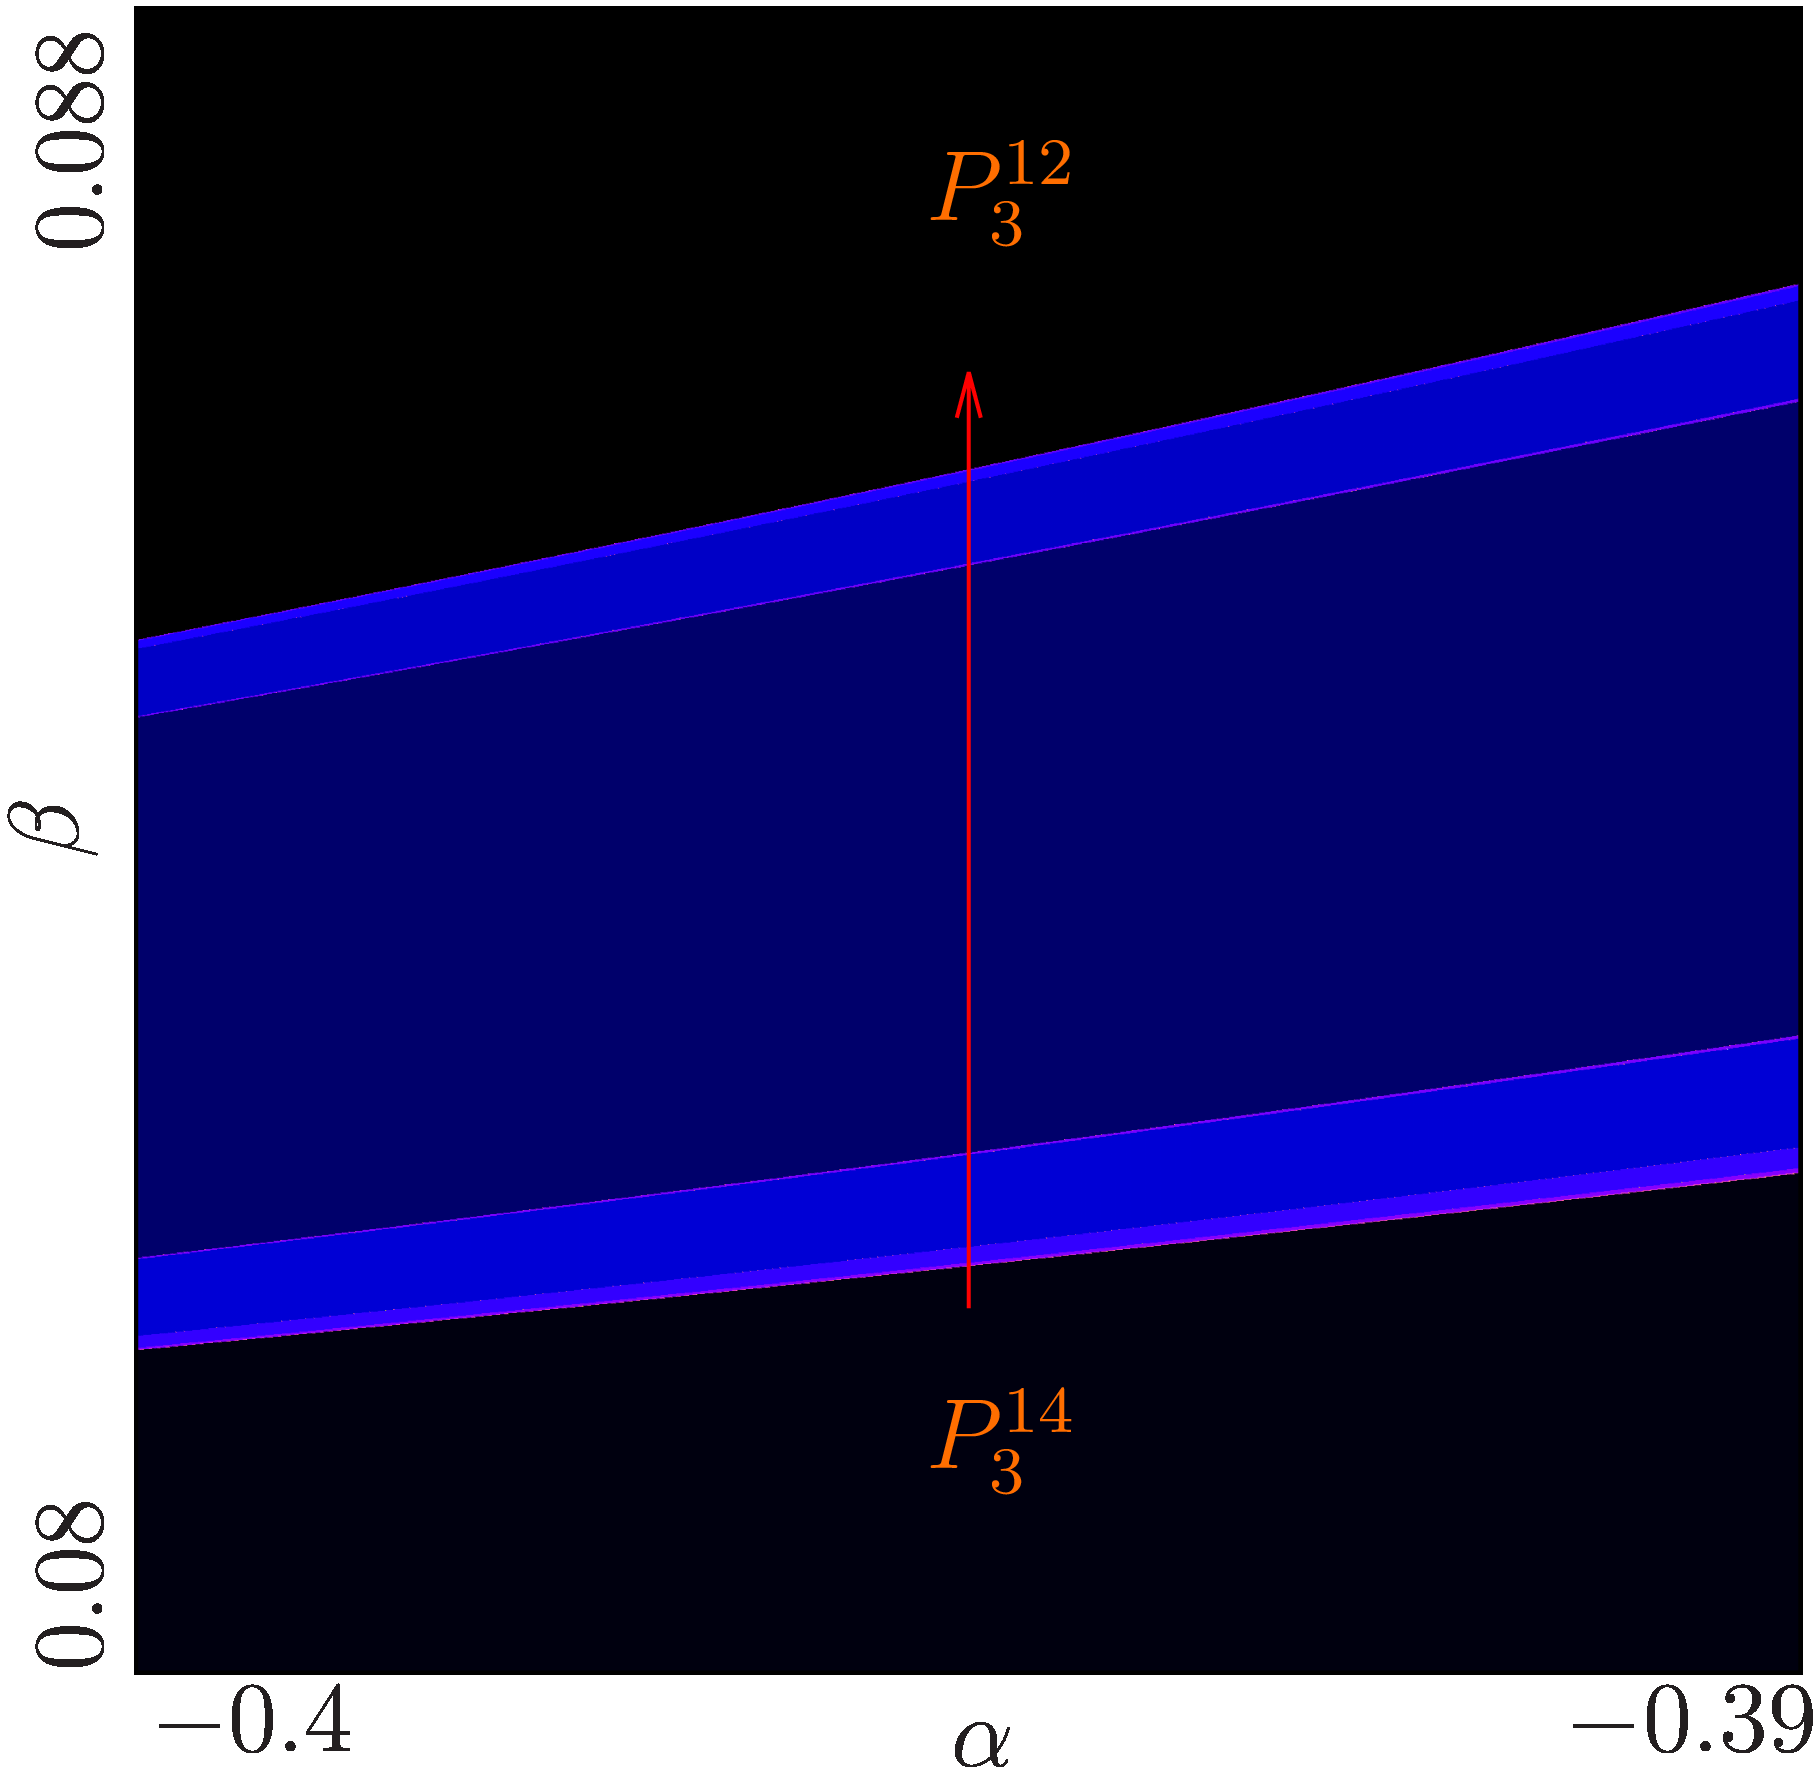
\includegraphics[width=.45 \textwidth]{../Figures/7/7.19a/result.png}
		\label{fig:add.halved.hor.2D}
	}
	\subfloat[1D period scan]{
		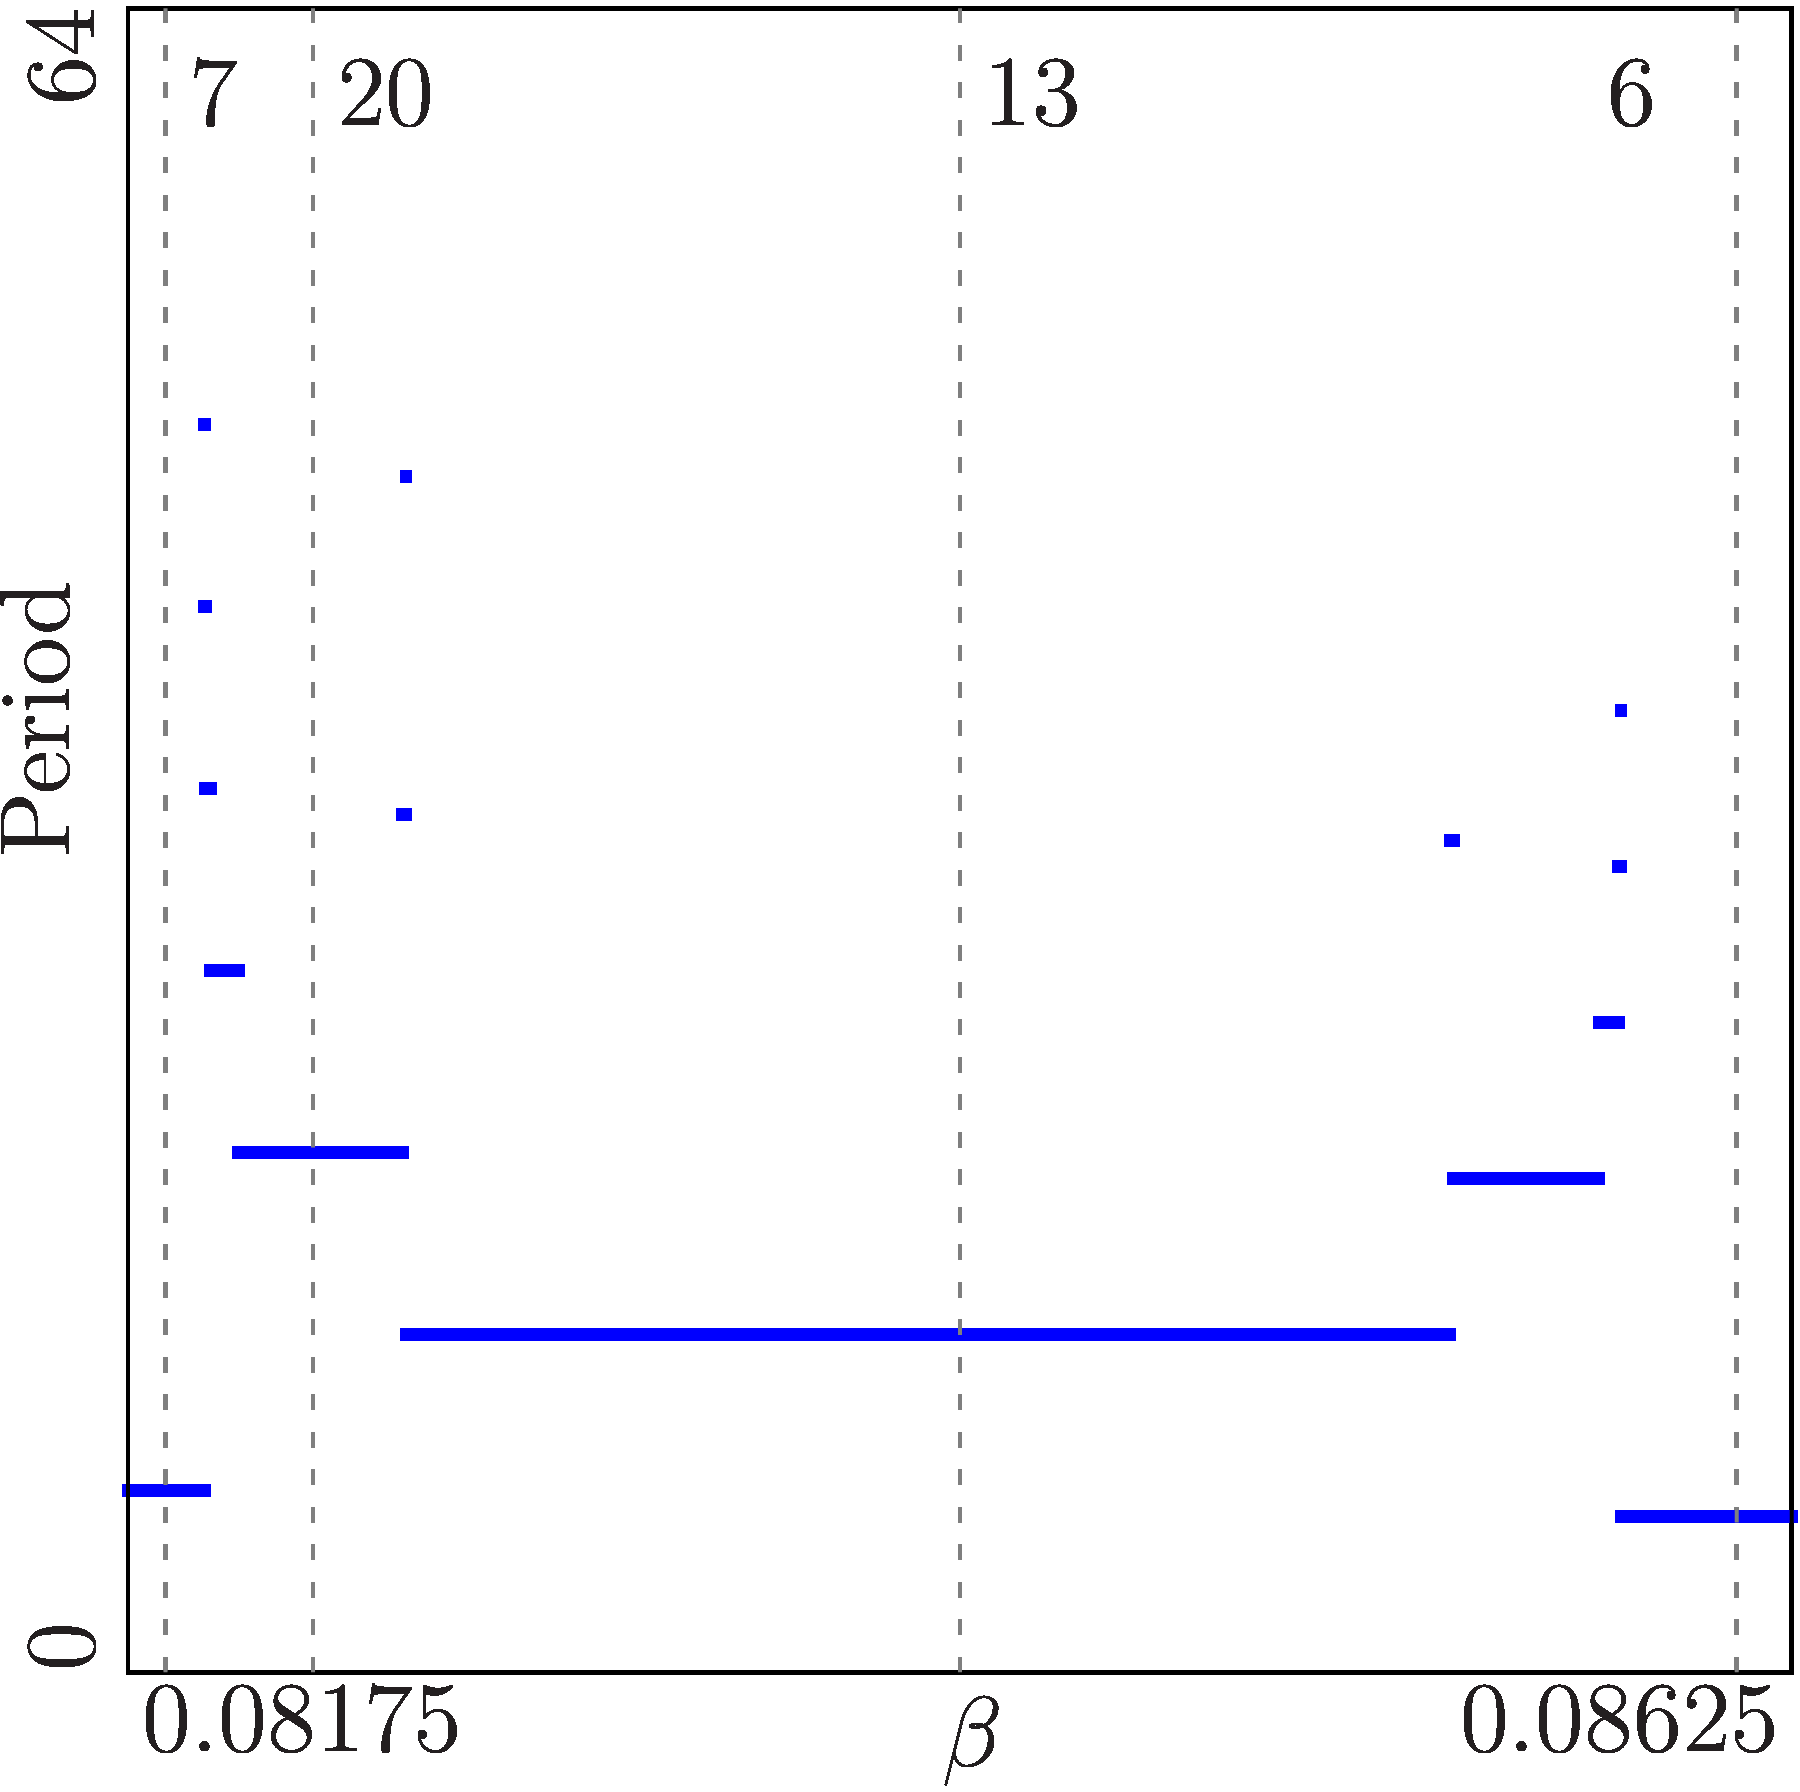
\includegraphics[width=.45 \textwidth]{../Figures/7/7.19b/result.png}
		\label{fig:add.halved.hor.1D}
	}
	\caption[2D and 1D scans of the periods associated with parameter regions in the halved archetypal model with increasing branches showing a horizontally oriented period-adding structure]{
		2D and 1D scans of the periods associated with parameter regions in the archetypal model with increasing branches showing a horizontally oriented \gls{pa} structure.
		The parameters $a_L = 1, b_L = 0.8,$ and $g_R\left(\frac{1}{2}\right) = \frac{1}{2} + \frac{1}{40}$ are fixed.
		The parameters $\alpha = g_R\left(\frac{1}{4}\right)$ and $\beta = c_L$ are different in each diagram.
		(a) shows the 2D scan where the parameters $\alpha$ and $\beta$ are varied in the ranges $[-0.4, -0.39]$ and $[0.08, 0.088]$
		and (b) shows the 1D scan where the parameter $\alpha = -0.395$ is fixed and $\beta$ is varied in the range $[0.08175, 0.08275]$ which is marked with a red arrow in (a).
	}
	\label{fig:add.add.halved.hor}
\end{figure}

As in the previous sections, the symbolic sequences of the cycles associated with the parameter regions in this structures are examined.
\Cref{fig:halved.hor.tree} shows the Farey-tree with the symbolic sequences associated with the parameter regions of this structure.
One can see that the symbolic sequence of a child node is the concatenation of the symbolic sequences of the parent nodes, as we would expect from \gls{pa} structures.
It turns out that the hybrid parameter region $\left[P^{14}_3 \mid P^{12}_3\right]$ was also part of the horizontal \gls{pal} structure described in \Cref{sec:add.add.like}.
And the \gls{pal} structures in the archetypal model are consequences of the \gls{pa} structures in the halved archetypal model.

\begin{figure}
	\centering
	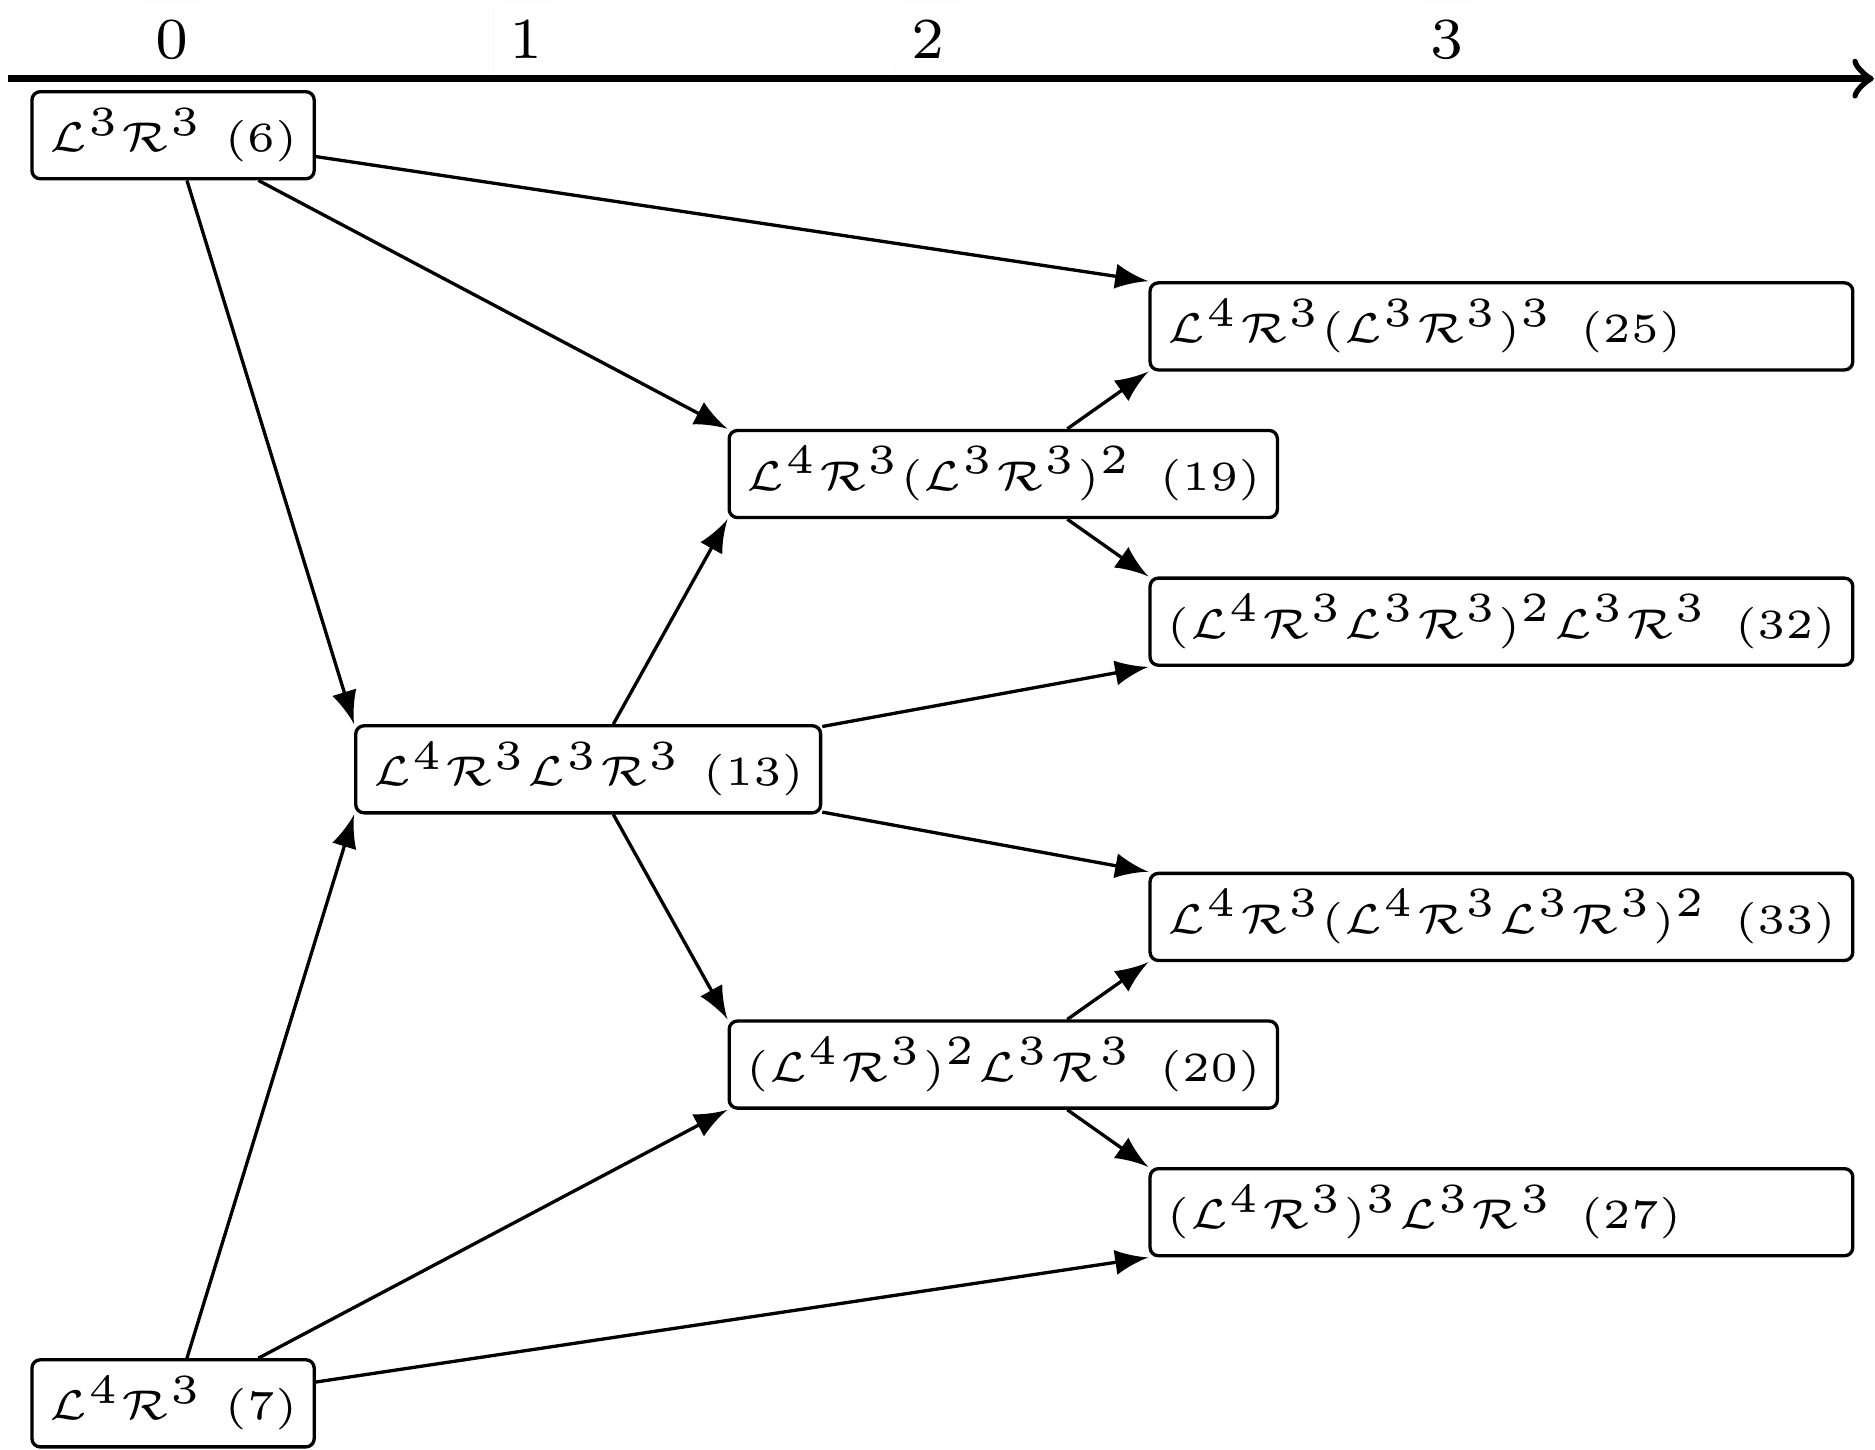
\includegraphics[width=.7 \textwidth]{../Figures/7/7.20/adding.png}
	\caption[Farey-tree showing the symbolic sequences of a horizontal \glsentrylong{pa} structure]{
		Farey-tree showing the symbolic sequences associated with the parameter regions of the horizontal \gls{pa} structure marked with a red arrow in \Cref{fig:add.halved.hor.2D} up to three levels.
		The periods associated with the parameter regions the cycles are in parentheses.
	}
	\label{fig:halved.hor.tree}
\end{figure}

The numerical evidence shows that the \gls{pa} structures in the halved archetypal model manifest as \gls{pal} structures in the archetypal model.
And the rules for the symbolic sequences of parameter regions in \gls{pa} structures are well known.
By formulating an algorithm that can translate symbolic sequences between the halved archetypal model and the archetypal model, one can generate the symbolic sequences of any \gls{pal} structure without the need for simlulating the archetypal model in every parameter region of the \gls{pal} structure.
Furthermore, with such an algorithm, one can derive rules for the \gls{pal} structures in the archetypal model from the rules for \gls{pa} structures.
The rules include rules for the periods, symbolic sequences, multistability, and even rotation numbers of the cycles associated with the parameter regions.

The next section introduces such algorithms and formulates some regularities in the translation of symbolic sequences.
With these algorithms and regularities, the rules for \gls{pal} structures in the archetypal model are derived later.

\subsection{Translating Symbolic Sequences}
\label{sec:add.halved.tanslating}

First, we define naive algorithms for translating symbolic sequences between the archetypal and the halved archetypal model based on the idea of the lifted model.
\hl{
	Then, we derive regularities for translated symbolic sequences in the archetypal model.
}
Finally, we refine the algorithms \hl{using the regularities of translated symbolic sequences}.

In the following, cycles of the archetypal model get the symbols $\phi, \psi,$ and $\pi$.
Cycles of the halved archetypal model get the symbols $\sigma, \rho,$ and $\tau$.
If there are two coexisting twin cycles, they are written as $\phi^a$ and $\phi^b$.
Also, the symbols for the symbolic sequences in the halved archetypal model are $\L$ and $\R$ instead of $\A, \B, \C,$ and $\D$ to avoid confusion.

\subsubsection{Naive Algorithms}

We start \hl{by} formulating a naive algorithm for translating symbolic sequences from the archetypal model to the halved archetypal model.
This is the easier direction.
From this algorithm we don't learn much about the nature of the \gls{pal} structures in the archetypal model.
The algorithm for translating symbolic sequences in the other direction, from the halved archetypal model to the archetypal model, will be more important for that.

To translate a symbolic sequence of the archetypal model we start by writing it down.
For example, \hl{let} $\phi = \A^4\B^3\C^4\D^3$.
Then we replace the symbols $\A$ and $\C$ by $\L$ and the symbols $\B$ and $\D$ by $\R$.
Now we have $\L^4\R^3\L^4\R^3$.
Finally, we have to check for redundancy in the resulting cycle.
In our example, the cycle $\L^4\R^3$ repeats twice in $\L^4\R^3\L^4\R^3$, so we just keep $\L^4\R^3$.

The opposite direction is trickier.
We start by writing down the symbolic sequence in the halved archetypal model.
For example $\sigma = \L^4\R^3\L4\R^3\L^3\R^3$.
Now we need to build pairs of rotations since each blue block fits exactly two red blocks.
If there is one rotation left over at the end, we wrap around or equivalently write down the original sequence again.
We repeat this until all rotations we have written down are paired up.

\begin{lemma}[How Often to Write Down the Symbolic Sequence]
	\label{lemma:writing.down}
	For cycles in the halved archetypal model $\sigma$ with an even number of rotations $n$, we only need to write the original cycle down once.
	For cycles in the halved archetypal model $\sigma$ with an odd number of rotations $n$, we need to write the original cycle down exactly twice.
\end{lemma}

\clearpage

\begin{proof} \phantom{x}
	\begin{enumerate}
		\item Let $n = 2i$. Then, we can build $i$ pairs of rotations and fit all $2i$ rotations of the original model.
		\item Let $n = 2i + 1$. We start by building $i$ pairs of rotations, fitting $2i$ rotations.
		      This will leave the last rotation unpaired, so we write down the sequence of $2i + 1$ rotations again.
		      Now we can pair up the last rotation of the first sequence we wrote down with the first rotation of the sequence we just wrote down.
		      $2i$ rotations remain, which we can fit into $i$ pairs.
	\end{enumerate}
	\hfill $\blacksquare$
\end{proof}

Notice that our example symbolic sequence has 3 rotations.
This means we have to write down the original sequence twice $\sigma^2 = \L^4\R^3\L4\R^3\L^3\R^3\L^4\R^3\L4\R^3\L^3\R^3$.

Then we pair up the rotations, this corresponds to drawing blue boxes around the red boxes in the infinite model.
In our example, we get the pairs $\left(\L^4\R^3\L^4\R^3\right)\left(\L^3\R^3\L^4\R^3\right)\left(\L^4\R^3\L^3\R^3\right)$.
The pairs then have to be translated using the function $t$ defined below in \Cref{def:t}.
The resulting symbolic sequence is $T(h) = \A^4\B^3\C^4\D^3\A^3\B^3\C^4\D^3\A^4\B^3\C^3\D^3$.
The formal definition of $T$ is below in \Cref{def:T}.

\begin{definition}[Syllables]
	A syllable is a maximal sequence of the same symbol of a symbolic sequence.
	A 2-syllable is a pair of syllables that are next to each other.
	And a 4-syllable is a pair of 2-syllables that are next to each other.
\end{definition}

So for example, the symbolic sequence $\L^4\R^3\L^3\R^3$ has 4 syllables.
Its syllables are $\L^4$, $\L^3$, and two times $\R^3$.
And a 2-syllable of the cycle is $\L^4\R^3$.
In the halved archetypal model, a 2-syllable corresponds to one rotation.
The 2-syllables of a cycle $\sigma$ in the halved archetypal model are written as $\sigma_i$.
In the archetypal model, a 4-syllable corresponds to one rotation.
The 4-syllables of a cycle $\phi$ in the archetypal model are written as $\phi_i$.
These terms are used interchangeably in the rest of this chapter.

\begin{definition}[Translating 4-syllables from Halved Archetypal to Archetypal]
	\label{def:t}
	The function $t$ maps two rotations, or a 4-syllable that starts with the symbol $\L$ of a symbolic sequence in the halved archetypal model to a single rotation in the archetypal model.
	It is defined in the following way.
	\begin{align}
		t: & \L^a\R^b\L^c\R^d \mapsto \A^a\B^b\C^c\D^d
	\end{align}
\end{definition}

\begin{definition}[Translating Symbolic Sequences from Halved Archetypal to Archetypal]
	\label{def:T}
	The function $T$ translates a symbolic sequence $\sigma = \sigma_1\sigma_2 \dots \sigma_n$ in the halved archetypal model to the archetypal model.
	Where $\sigma_i$ are the 2-syllables of $\sigma$.
	From \Cref{lemma:writing.down} we know how often we need to write down $\sigma$, and therefore also which 4-syllables to translate with $t$.
	\begin{align}
		T(\sigma) & = \begin{cases}
			              t(\sigma_1\sigma_2) \dots t(\sigma_{n-1}\sigma_n)                           & \text{ if } n | 2 \\
			              t(\sigma_1\sigma_2) \dots t(\sigma_n\sigma_1) \dots t(\sigma_{n-1}\sigma_n) & \text{ else }
		              \end{cases}
	\end{align}
\end{definition}

\begin{definition}[Shifting Symbolic Sequences]
	The function $s_2$ shifts a symbolic sequence $\sigma$ in the halved archetypal model by a single rotation, or equivalently by a 2-syllable.
	Let $\sigma = \sigma_1\sigma_2 \dots \sigma_n$.
	Then $s_2$ is defined in the following way.
	\begin{align}
		s_2: & \sigma_1\sigma_2 \dots \sigma_n \mapsto \sigma_2 \dots \sigma_n\sigma_1
	\end{align}
	In the archetypal model, there is a similar function, $s_4$ that shifts a symbolic sequence $\phi$ in the archetypal model by a single rotation.
	Let $\phi = \phi_1\phi_2 \dots \phi_n$.
	Then $s_4$ is defined in the following way.
	\begin{align}
		s_4: & \phi_1\phi_2 \dots \phi_n \mapsto \phi_2 \dots \phi_n\phi_1
	\end{align}
\end{definition}

\begin{definition}[Shift-equivalence]
	The two symbolic sequences $\phi$ and $\psi$ in the archetypal model are shift-equivalent $\phi \equiv \psi$,
	if they both have the same number of rotations $n$
	and there is a number $0 \leq i < n$, such that $\phi = s_4^i(\psi)$.
	Where $s_4^i(\psi)$ is defined as $s_4^{i-1}(s_4(\psi))$ and $s_4^1(\psi) = s_4(\psi)$.
\end{definition}

We need to repeat the whole process for each shift $s_2^i$ of the original symbolic sequence for $0 < i < n$ where $n$ is the number of 2-syllables of the original symbolic sequence.
And we only keep the results that are not shift-equivalent to any previous result, since shift-equivalent cycles are identical in the archetypal model.
In our example, we would repeat the process for $s_2(\sigma) = \L^4\R^3\L3\R^3\L^4\R^3$ and get the result $T(s_2(\sigma)) = \A^4\B^3\C^3\D^3\A^4\B^3\C^4\D^3\A^3\B^3\C^4\D^3$.
This result is shift-equivalent to the first result by shifting it 2 times ($s_4^2$).
Last we need to repeat it for $s_2^2(\sigma) = \L^3\R^3\L4\R^3\L^4\R^3$ and get the result $T(s_2^2(\sigma)) = \A^3\B^3\C^4\D^3\A^4\B^3\C^3\D^3\A^4\B^3\C^4\D^3$.
This result is shift-equivalent to the first result by shifting it once ($s_4$).

Therefore, the cycle $\sigma$ in the halved archetypal model manifests as a single cycle $T(\sigma)$ in the archetypal model.
We write it as $F(\sigma) = \{T(\sigma)\} = \{\A^4\B^3\C^4\D^3\A^3\B^3\C^4\D^3\A^4\B^3\C^3\D^3\}$.
The result of $F$ is a set because the cycle $\sigma$ in the halved archetypal model may manifest as multiple coexisting cycles in the archetypal model.

\subsubsection{Properties of Translated Symbolic Sequences in the Full Model}

With this naive algorithm, we can start to investigate rules for the \gls{pal} structures in the archetypal model.

\begin{lemma}[Shif-equivalence of Translated Symbolic Sequences in the Archetypal Model]
	\label{lemma:equivalence.translations}
	The translations of the two cycles $\sigma$ and $\rho = s_2^{2i}(\sigma)$ in the halved archetypal model are shift-equivalent $T(\sigma) \equiv T(\rho)$ in the archetypal model for all integers $i$.
\end{lemma}

\begin{proof} \phantom{x} \\
	Let $\sigma = \sigma_1\sigma_2 \dots \sigma_n$, therefore $\rho = \sigma_{2i+1} \dots \sigma_n\sigma_1 \dots \sigma_{2i}$.
	The translations are $T(\sigma) = t(\sigma_1\sigma_2)t(\sigma_3\sigma_4) \dots t(\sigma_{n-1}\sigma_n)$
	and $T(\rho) = t(\sigma_{2i+1}\sigma_{2i+2}) \dots t(\sigma_{n-1}\sigma_n)t(\sigma_1\sigma_2) \dots t(\sigma_{2i-i}\sigma_{2i})$.
	We can see that $T(\rho) = s_4^i(T(\sigma))$ and therefore $T(\sigma) \equiv T(\rho)$.

	\hfill $\blacksquare$
\end{proof}

\clearpage

\begin{theorem}[Coexistence of Translated Symbolic Sequences in the Archetypal Model]
	\label{theorem:coexistence.even}
	The manifestations of a cycle in the halved archetypal model $\sigma$ is either $F(\sigma) = \{T(\sigma), T(s_2(\sigma))\}$ or $F(\sigma) = \{T(\sigma)\}$.
	And \begin{enumerate}
		\item $F(\sigma) = \{T(\sigma), T(s_2(\sigma))\}$ if the number of rotations of the sequence $\sigma$ is even.
		\item $F(\sigma) = \{T(\sigma)\}$ if the number of rotations of the sequence $\sigma$ is odd.
	\end{enumerate}
\end{theorem}

\begin{proof} \phantom{x} \\
	Let $\sigma = \sigma_1\sigma_2 \dots \sigma_n$ a symbolic sequence in the halved archetypal model with $n$ rotations.
	We know from \Cref{lemma:equivalence.translations} that the only possible candidates for $F(\sigma)$ are $T(\sigma)$ and $T(s_2(\sigma))$.
	These are the first two possibilities we check in the algorithm and all other shifts $T(s_2^i(\sigma))$ with $2 \leq i < n$ are shift-equivalent to either $T(\sigma)$ or $T(s_2(\sigma))$.
	This follows directly from \Cref{lemma:equivalence.translations}.
	So, in the following, we will only check for the shift-equivalence of these two candidates.
	\begin{enumerate}
		\item Let $n = 2i$.
		      \begin{align*}
			      T(h)                 & = t(\sigma_1\sigma_2) t(\sigma_3\sigma_4) \dots t(\sigma_{n-1}\sigma_n) \\
			      \nequiv \: T(s_2(h)) & = t(\sigma_2\sigma_3) t(\sigma_4\sigma_5) \dots t(\sigma_n\sigma_1)
		      \end{align*}
		      The two candidates are not shift-equivalent because the pair $t(\sigma_1\sigma_2)$ in $T(\sigma)$ is not included in the other candidate $T(s_2(\sigma))$.
		      The same is true for any other pair, and therefore $F(\sigma) = \{T(\sigma), T(s_2(\sigma))\}$.
		\item Let $n = 2i + 1$.
		      \begin{align*}
			      T(h)                & = t(\sigma_1\sigma_2) t(\sigma_3\sigma_4) \dots t(\sigma_n\sigma_1) t(\sigma_2\sigma_3) \dots t(\sigma_{n-1}\sigma_n) \\
			      \equiv \: T(s_2(h)) & = t(\sigma_2\sigma_3) \dots t(\sigma_{n-1}\sigma_n) t(\sigma_1\sigma_2) t(\sigma_3\sigma_4) \dots t(\sigma_n\sigma_1)
		      \end{align*}
		      The two candidates are shift-equivalent.
		      By shifting the second candidate $T(s_2(\sigma))$ $2i$ times, we get the first candidate $T(\sigma)$.
		      Therefore, the second candidate is discarded and $F(\sigma) = \{T(\sigma)\}$.
	\end{enumerate}
	\hfill $\blacksquare$
\end{proof}

Note that a result of $F(\sigma) = \{T(\sigma), T(s_2(\sigma))\}$ means that the cycle $\sigma$ in the halved archetypal model manifests as two coexisting cycles in the archetypal model.

\subsubsection{Revised Algorithms}

With all these properties and functions we now can formulate a more compact algorithm, \Cref{alg:halved.to.full}, for translating symbolic sequences from the halved archetypal model into the archetypal model.
This revised algorithm will be used in the following to construct the rules for the \gls{pal} structures in the archetypal model.

\begin{algorithm}
	\caption{Algorithm for the Translation of Symbolic Sequences from the Halved Archetypal Model to the Archetypal Model}\label{alg:halved.to.full}
	\begin{algorithmic}
		\Require $\sigma = \sigma_1\sigma_2 \dots \sigma_n$ with $n > 0$
		\If{$n$ is even}
		\State \Return $\{t(\sigma_1\sigma_2) t(\sigma_3\sigma_4) \dots t(\sigma_{n-1}\sigma_n), t(\sigma_2\sigma_3) t(\sigma_4\sigma_5) \dots t(\sigma_n\sigma_1)\}$
		\ElsIf{$n$ is odd}
		\State \Return $\{t(\sigma_1\sigma_2) \dots t(\sigma_{n}\sigma_1) \dots t(\sigma_{n-1}\sigma_n)\}$
		\EndIf
	\end{algorithmic}
\end{algorithm}

\Cref{alg:full.to.halved} shows the inverse algorithm for translating symbolic sequences from the archetypal model to the halved archetypal model for completeness.
It uses the inverse $t^{-1}$ of the function $t$.

\begin{definition}[Translating 4-syllables from Archetypal to Halved Archetypal]
	The function $t^{-1}$ maps a 4-syllable of a symbolic sequence in the archetypal model to the halved archetypal model.
	It is defined in the following way.
	\begin{align}
		t^{-1}: \quad \A^a\B^b\C^c\D^d \mapsto \L^a\R^b\L^c\R^d
	\end{align}
\end{definition}

\begin{algorithm}
	\caption{Algorithm for the Translation of Symbolic Sequences from the Halved Model to the Halved Archetypal Model}\label{alg:full.to.halved}
	\begin{algorithmic}
		\Require $\phi = \phi_1\phi_2 \dots \phi_n$ with $n > 0$
		\State $d \gets t^{-1}(\phi_1)t^{-1}(\phi_2) \dots t^{-1}(\phi_n) = \sigma_1\sigma_2 \dots \sigma_m$
		\Comment $m = 2n$ is even
		\State $\tau \gets \sigma_1\sigma_2 \dots \sigma_{\frac{m}{2}}$
		\If{$\sigma = \tau^2$}
		\State \Return $\tau$
		\ElsIf{$\sigma \neq \tau^2$}
		\State \Return $\sigma$
		\EndIf
	\end{algorithmic}
\end{algorithm}

\subsection{Properties of the \Glsentrylong{pal} Structures in the Archetypal Model}
\label{sec:add.rules.pal}

With the revised algorithms we can now explain the \gls{pal} structures in the archetypal model.
We start by explaining why some cycles have a much higher period than expected in the \gls{pal} structures.
After that, we construct rules for the symbolic sequences in the \gls{pal} structures in the archetypal model.
And finally, we construct rules for the rotation-like numbers in the \gls{pal} structures in the archetypal model.

\subsubsection{Periods in the \Glsentrylong{pal} Structures}

First, we state that the function $t$ that translates 4-syllables from the halved archetypal model to the archetypal model preserves the period of the 4-syllable.
The function was defined in \Cref{sec:add.halved.tanslating}.

\begin{lemma}[$t$ Preserves Period]
	\label{lemma:t.preserves.period}
	The function $t$ preserves the period.
	\begin{align}
		|\sigma_1\sigma_2| = |t(\sigma_1\sigma_2)|
	\end{align}
\end{lemma}

\begin{proof}
	Let $\sigma_1\sigma_2 = \L^a\R^b\L^c\R^d$.
	\begin{align*}
		|\sigma_1\sigma_2| =  |\L^a\R^b\L^c\R^d|
		= a + b + c + d
		= |\A^a\B^b\C^c\D^d|
		= |t(\L^a\R^b\L^c\R^d)|
		= |t(\sigma_1\sigma_2)|
	\end{align*}
	\hfill $\blacksquare$
\end{proof}

\begin{theorem}[Period of Cycles in the Full Model]
	\begin{enumerate}
		\item If a cycle in the halved model manifests as two coexisting cycles in the full model, the period of either cycle is the same as the period of the cycle in the halved model.
		      \begin{align*}
			      |T(\sigma)| = |T(s_2(\sigma))| = |\sigma|
		      \end{align*}
		\item If a cycle in the halved model manifests as a single cycle in the full model, the period of this cycle is double the period of the cycle in the halved model.
		      \begin{align*}
			      |T(\sigma)| = 2 |\sigma|
		      \end{align*}
	\end{enumerate}
\end{theorem}

\clearpage

\begin{proof} \phantom{x}
	\begin{enumerate}
		\item From \Cref{theorem:coexistence.even} we know that if the cycle $\sigma$ in the halved model manifests as two coexisting cycles in the full model, $\sigma$ has an even number of rotations $n$.
		      And its translation is $T(\sigma) = t(\sigma_1\sigma_2) t(\sigma_3\sigma_4) \dots t(\sigma_{n-1}\sigma_n)$.
		      Combining this with the fact, that $t$ preserves the period of its input as described in \Cref{lemma:t.preserves.period}, we can calculate the period of $T(\sigma)$ in the following way.
		      \begin{align*}
			      |T(\sigma)| & = |t(\sigma_1\sigma_2) t(\sigma_3\sigma_4) \dots t(\sigma_{n-1}\sigma_n)|           \\
			                  & = |t(\sigma_1\sigma_2)| + |t(\sigma_3\sigma_4)| + \dots + |t(\sigma_{n-1}\sigma_n)| \\
			                  & = |\sigma_1\sigma_2| + |\sigma_3\sigma_4| + \dots + |\sigma_{n-1}\sigma_n|          \\
			                  & = |\sigma_1\sigma_2 \dots \sigma_n| = |\sigma|
		      \end{align*}
		      So the period of the cycle $T(\sigma)$ in the archetypal model is the same as the period of the cycle $\sigma$ in the halved archetypal model.
		      The same calculation can be done for $T(s(\sigma))$ and is omitted here.
		\item Similarly, we know that if the cycle $\sigma$ in the halved model manifests as a single cycle in the full model, $\sigma$ has an odd number of rotations $n$.
		      And its translation is $T(\sigma) = t(\sigma_1\sigma_2) \dots t(\sigma_n\sigma_1) \dots t(\sigma_{n-1}\sigma_n)$.
		      Its period can be calculated in the following way.
		      \begin{align*}
			      |T(\sigma)| & = |t(\sigma_1\sigma_2) \dots t(\sigma_n\sigma_1) \dots t(\sigma_{n-1}\sigma_n)|                      \\
			                  & = |t(\sigma_1\sigma_2)| + \dots + |t(\sigma_n\sigma_1)| + \dots + |t(\sigma_{n-1}\sigma_n)|          \\
			                  & = |\sigma_1\sigma_2| + \dots + |\sigma_n\sigma_1| + \dots + |\sigma_{n-1}\sigma_n|                   \\
			                  & = |\sigma_1\sigma_2 \dots \sigma_n\sigma_1 \dots \sigma_{n-1}\sigma_n| = |\sigma\sigma| = 2 |\sigma|
		      \end{align*}
		      So the period of the cycle $T(\sigma)$ in the full model is twice the period of the cycle $\sigma$ in the halved model.
	\end{enumerate}
	\hfill $\blacksquare$
\end{proof}

\todo{\Cref{lemma:t.preserves.period} should be Lemma 7.5}

With this property we can also explain the regularities for coexistence of two cycles in the Farey-trees of \gls{pal} structures.
\todo{Here Farey-tree of full horizontal pal structure}

The third case in \Cref{theorem:child.coexistence} can't be seen in the farey tree but it follows from the proof of the first two cases.
\todo{Last case not possible in our adding structures. proof!}

\begin{theorem}[Multiplicity of Cycles Associated With Child Nodes Based on the Multiplicity of Cycles Associated With its Parent Nodes]
	\label{theorem:child.coexistence}
	\begin{enumerate}
		\item The child of a node with a single cycle and a node with two coexisting cycles has a single cycle.
		\item The child of two nodes with a single cycle has two coexisting cycles.
		\item The child of two nodes with two coexisting cycles, has two coexisting cycles.
	\end{enumerate}
\end{theorem}

\begin{proof} \phantom{x}
	\begin{enumerate}
		\item A node with a single cycle in the full model is the manifestation of a cycle with an odd number of rotations in the halved model.
		      A node with two coexisting cycles in the full model is the manifestation of a cycle with an even number of rotations in the halved model.
		      Their child is the manifestation of the two cycles in the halved model glued together.
		      This glued-together cycle has an odd number of rotations and therefore manifests as a single cycle in the full model.
		\item Analogously, two cycles with an odd number of rotations glued together have an even number of rotations.
		      Therefore, this glued-together cycle manifests as two coexisting cycles in the full model.
		\item Analogously, two cycles with an even number of rotations glued together have an even number of rotations.
		      Therefore this glued-together cycle manifests as two coexisting cycles in the full model.
	\end{enumerate}
\end{proof}


This explains the pattern we observed in the periods of the \gls{pal} structures in \Cref{sec:add.add.like}.
We take another look at the 1D period scan of the horizontal \gls{pal} structure between the parameter regions $P^{14}_3$ and $\left[P^{14}_3  \mid P^{12}_3\right]$ in \Cref{fig:add.add.like.hor.1D}.
We get the information, whether a parameter region in the structure was associated with two coexisting cycles from the Farey-tree in \Cref{fig:add.add.like.hor.tree}.
The parameter region associated with the period $14$ is not associated with coexisting cycles, therefore the corresponding cycle in the halved archetypal model has an odd number of revolutions and its period is twice as high as the period associated with the same parameter region in the halved archetypal model, which is $7$.
The parameter region associated with the period $13$ is associated with coexisting cycles, therefore the corresponding cycle in the halved archetypal model has an even number of revolutions its period is the same as the period associated with the same parameter region in the halved archetypal mode.
The parameter region in between those two parameter regions is associated with the period $7 + 13 = 20$ in the halved archetypal model.
Also, its cycle has an odd number of revolutions, since it is the concatenation of one cycle with an even and one cycle with an odd number of revolutions.
We know from \Cref{theorem:period.pal} that this parameter region is associated with the period $40$ in the archetypal model.
This is true as we can observer this in the 1D period scan in \Cref{fig:add.add.hor.1D}.
Also, we know from \Cref{theorem:child.coexistence} that this parameter region is associated with two coexisting cycles.
This is true as we can see in the Farey-tree \todo{reference tree}

\todo{1D period scan again?}

\subsubsection{Rules for Combining Symbolic Sequences}

Furthermore, we can formulate rules for the cycles in the child node of two nodes in the period-adding structure in the full model.

\begin{definition}[Merging two 4-syllables]
	The operation $\left[\phi_i \mid \psi_j\right]$ merges the two 4-symmables $\phi_i$ and $\psi_j$.
	Let $\phi_i = \A^a\B^b\C^c\D^d$ and $\psi_j = \A^e\B^f\C^g\D^h$.
	Then $\left[\phi_i \mid \psi_j\right] = \A^a\B^b\C^g\D^h$.
	It concatenates the first 2-syllable of $\phi_i$ with the second 2-syllable of $\psi_j$.
\end{definition}

\begin{theorem}[The Cycles of a Child Node of a Node With a Singular Cycle and a Node With 2 Coexisting Cycles]
	The child node of a node with a singular cycle $\phi = \phi_1\phi_2 \dots \phi_n$ and a node with two coexisting cycles $\phi^a = \phi^a_1\phi^a_2 \dots \phi^a_m$ and $\phi^b_1\phi^b_2 \dots \phi^b_m$ will have one of the following cycles.
	\begin{enumerate}
		\item If $\phi$ is associated with the left parent.
		      \begin{align*}
			      \phi_1 \dots \phi_{\frac{n-1}{2}} \left[\phi_{\frac{n+1}{2}} \mid \phi^b_m\right]
			      \phi^b_1 \dots \phi^b_{m-1} \left[\phi^b_m \mid \phi_{\frac{n+1}{2}}\right]
			      \phi_{\frac{n+3}{2}} \dots \phi_n \phi^a
		      \end{align*}
		\item If $\phi$ is associated with the right parent.
		      \begin{align*}
			      \phi^a \phi_1 \dots \phi_{\frac{n-1}{2}} \left[\phi_{\frac{n+1}{2}} \mid \phi^b_m\right]
			      \phi^b_1 \dots \phi^b_{m-1} \left[\phi^b_m \mid \phi_{\frac{n+1}{2}}\right]
			      \phi_{\frac{n+3}{2}} \dots \phi_n
		      \end{align*}
		      Which is shift-equivalent to the first case.
		      But this distinction must be made to guarantee the correctness of cycles in subsequent child nodes.
	\end{enumerate}
\end{theorem}

\begin{proof} \phantom{x}
	\begin{enumerate}
		\item Let $\sigma = \sigma_1\sigma_2 \dots \sigma_i$ with odd $i$ and $\rho = \rho_1\rho_2 \dots \rho_j$ with even $j$ and $T(\sigma) = \phi, T(\rho) = \psi^a$, and $T(s_2(\rho)) = \psi^b$.
		      The child of both nodes in the halved model will have the cycle $\sigma\rho = \sigma_1\sigma_2 \dots \sigma_i \rho_1\rho_2 \dots \rho_j$.
		      This will manifest as the following cycle in the full model.
		      \begin{align*}
			      T(\sigma\rho) & = T(\sigma_1 \dots \sigma_i \rho_1 \dots \rho_j)                                                                              \\
			                    & =
			      t(\sigma_1\sigma_2) \dots t(\sigma_i \rho_1) \dots t(\rho_j \sigma_1) \dots t(\sigma_{i-1}\sigma_i) t(\rho_1\rho_2) \dots t(\rho_{j-1}\rho_j) \\
			                    & = \phi_1 \dots \phi_{\frac{n-1}{2}} t(\sigma_i \rho_1)
			      \psi^b_1 \dots \rho^b_{m-1} t(\rho_j \sigma_1)
			      \phi_{\frac{n+3}{2}} \dots \phi_n
			      \psi^a_1 \dots \psi^a_m                                                                                                                       \\
			                    & =
			      \phi_1 \dots \sigma_{\frac{n-1}{2}} \left[\sigma_{\frac{n+1}{2}} \mid \rho^b_m\right]
			      \psi^b_1 \dots \psi^b_{m-1} \left[\rho^b_m \mid \sigma_{\frac{n+1}{2}}\right]
			      \phi_{\frac{n+3}{2}} \dots \phi_n
			      \psi^a                                                                                                                                        \\
		      \end{align*}
		\item Let $\sigma = \sigma_1\sigma_2 \dots \sigma_i$ with even $i$ and $\rho = \rho_1\rho_2 \dots \rho_j$ with odd $j$ and $T(\sigma) = \psi^a, T(s_2(\sigma)) = \psi^b$, and $T(\rho) = \phi$.
		      The child of both nodes in the halved model will have the cycle $\sigma\rho = \sigma_1l_2 \dots \sigma_i \rho_1\rho_2 \dots \rho_j$.
		      This will manifest as the following cycle in the full model.
		      \begin{align*}
			      T(\sigma\rho) & = T(\sigma_1 \dots \sigma_i \rho_1 \dots \rho_j)                                                                                             \\
			                    & =
			      t(\sigma_1\sigma_2) \dots t(\sigma_{i-1}\sigma_i) t(\rho_1\rho_2) \dots t(\rho_j \sigma_1) \dots t(\sigma_i\rho_1) \dots t(\rho_j\sigma_1) \dots t(\sigma_i) \\
			                    & =
			      \psi^a_1 \dots \psi^a_m
			      \phi_1 \dots \phi_{\frac{n-1}{2}} t(\sigma_i \rho_1)
			      \psi^b_1 \dots \psi^b_{m-1} t(\rho_j \sigma_1)
			      \phi_{\frac{n+3}{2}} \dots \phi_n                                                                                                                            \\
			                    & =
			      \psi^a
			      \phi_1 \dots \phi_{\frac{n-1}{2}} \left[\phi_{\frac{n+1}{2}} \mid \psi^b_m\right]
			      \psi^b_1 \dots \psi^b_{m-1} \left[\psi^b_m \mid \phi_{\frac{n+1}{2}}\right]
			      \phi_{\frac{n+3}{2}} \dots \phi_n                                                                                                                            \\
		      \end{align*}
	\end{enumerate}
\end{proof}

\begin{theorem}
	The child node of two nodes with a singular cycle, $\phi = \phi_1 \dots \phi_n$ and $\psi = \psi_1 \dots \psi_m$ respectively, has the following two cycles.
	\begin{align*}
		\phi_1 \dots \phi_{\frac{n-1}{2}} \left[\phi_{\frac{n+1}{2}} \mid \psi_{\frac{m+1}{2}}\right] \psi_{\frac{m+3}{2}} \dots \psi_m
	\end{align*}
	and
	\begin{align*}
		\phi_{\frac{n+3}{2}} \dots \phi_n \psi_1 \dots \psi_{\frac{m-1}{2}} \left[\psi_{\frac{m+1}{2}} \mid \phi_{\frac{n+1}{2}}\right]
	\end{align*}
\end{theorem}

\begin{proof}
	Let $\sigma = \sigma_1\sigma_2 \dots \sigma_i$ with odd $i$ and $\rho = \rho_1\rho_2 \dots \rho_j$ with odd $j$ and $T(\sigma) = \phi$ and $T(\rho) = \psi$.
	The child of both nodes in the halved model will have the cycle $\sigma\rho = \sigma_1 \dots \sigma_i \rho_1 \dots \rho_j$.
	This will manifest as the following two cycles in the full model.
	\begin{align*}
		T(\sigma\rho) & = T(\sigma_1 \dots \sigma_i \rho_1 \dots \rho_j)                                                                                  \\
		              & = t(\sigma_1\sigma_2) \dots t(\sigma_i\rho_1) \dots t(\rho_{j-1}\rho_j)                                                           \\
		              & = \phi_1 \dots \phi_{\frac{n-1}{2}} t(\sigma_i\rho_1) \psi_{\frac{m+3}{2}} \dots \psi_j                                           \\
		              & = \phi_1 \dots \phi_{\frac{n-1}{2}} \left[\phi_{\frac{n+1}{2}} \mid \psi_{\frac{m+1}{2}}\right] \psi_{\frac{m+3}{2}} \dots \psi_j
	\end{align*}
	and
	\begin{align*}
		T(s(\sigma\rho)) & = T(\sigma_2 \dots \sigma_i \rho_1 \dots \rho_j \sigma_1)                                                                         \\
		                 & = t(\sigma_2\sigma_3) \dots t(\sigma_{i-1}\sigma_i) t(\rho_1\rho_2) \dots t(\rho_j\sigma_1)                                       \\
		                 & = \phi_{\frac{n+3}{2}} \dots \phi_n \psi_1 \dots \psi_{\frac{m-1}{2}} t(\rho_j\sigma_1)                                           \\
		                 & = \phi_{\frac{n+3}{2}} \dots \phi_n \psi_1 \dots \psi_{\frac{m-1}{2}} \left[\psi_{\frac{m+1}{2}} \mid \phi_{\frac{n+1}{2}}\right]
	\end{align*}
\end{proof}

\todo{last case not possible in our adding structures. proof!}

As mentioned before, the next case does not appear in the fare tree in \Cref{fig:tree.adding1.hor.full}.
But we will include it here for completeness.

\begin{theorem}
	The child node of two nodes with two coexisting cycles each, $\{\phi^a, \phi^b\}$ and $\{\phi^a, \phi^b\}$ respectively, has the following two cycles.
	\begin{align*}
		\phi^a\phi^a \qquad \text{and} \qquad
		\phi^b_1 \dots \phi^b_{n-1} \left[\phi^b_n \mid \phi^b_m\right] \phi^b_1 \dots \phi^b_{m-1} \left[\phi^b_m \mid \phi^b_n\right]
	\end{align*}
\end{theorem}

\begin{proof}
	Let $\sigma = \sigma_1 \dots \sigma_i$ with even $i$ and $\rho = \rho_1 \dots \rho_j$ with even $j$ and $T(\sigma) = \phi^a, T(s_2(\sigma)) = \phi^b, T(\rho) = \phi^a$, and $T(s_2(\rho)) = \phi^b$.
	The child of both nodes in the halved model will have the cycle $\sigma\rho$.
	This will manifest as the following two cycles in the full model.
	\begin{align*}
		T(\sigma\rho) & = T(\sigma_1 \dots \sigma_i \rho_1 \dots \rho_j) = t(\sigma_1\sigma_2) \dots t(\sigma_{i-i}\sigma_i) t(\rho_1\rho_2) \dots t(\rho_{j-1}\rho_j) \\
		              & = \phi^a_1 \dots \phi^a_n \phi^a_1 \dots \phi^a_m = \phi^a\phi^a
	\end{align*}
	and
	\begin{align*}
		T(s(\sigma\rho)) & = T(\sigma_2 \dots \sigma_i \rho_1 \dots \rho_j \sigma_1) = t(\sigma_2\sigma_3) \dots t(\sigma_i\rho_1) \dots t(\rho_j\sigma_1)   \\
		                 & = \phi^b_1 \dots \phi^b_{n-1} t(\sigma_i\rho_1) \phi^b_1 \dots \phi^b_{m-1} t(\rho_j\sigma_1)                                     \\
		                 & = \phi^b_1 \dots \phi^b_{n-1} \left[\phi^b_n \mid \phi^b_m\right] \phi^b_1 \dots \phi^b_{m-1} \left[\phi^b_m \mid \phi^b_n\right]
	\end{align*}
\end{proof}


